%%
%% This is file `sample-sigconf.tex',
%% generated with the docstrip utility.
%%
%% The original source files were:
%%
%% samples.dtx  (with options: `all,proceedings,bibtex,sigconf')
%%
%% IMPORTANT NOTICE:
%%
%% For the copyright see the source file.
%%
%% Any modified versions of this file must be renamed
%% with new filenames distinct from sample-sigconf.tex.
%%
%% For distribution of the original source see the terms
%% for copying and modification in the file samples.dtx.
%%
%% This generated file may be distributed as long as the
%% original source files, as listed above, are part of the
%% same distribution. (The sources need not necessarily be
%% in the same archive or directory.)
%%
%%
%% Commands for TeXCount
%TC:macro \cite [option:text,text]
%TC:macro \citep [option:text,text]
%TC:macro \citet [option:text,text]
%TC:envir table 0 1
%TC:envir table* 0 1
%TC:envir tabular [ignore] word
%TC:envir displaymath 0 word
%TC:envir math 0 word
%TC:envir comment 0 0
%%
%%
%% The first command in your LaTeX source must be the \documentclass
%% command.
%%
%% For submission and review of your manuscript please change the
%% command to \documentclass[manuscript, screen, review]{acmart}.
%%
%% When submitting camera ready or to TAPS, please change the command
%% to \documentclass[sigconf]{acmart} or whichever template is required
%% for your publication.
%%
%%
\documentclass[sigconf,nonacm]{acmart}

\usepackage{amsmath}
\usepackage{amsthm}
\usepackage{amsfonts}
\usepackage[linesnumbered,ruled,vlined]{algorithm2e}
\usepackage{xspace}
\usepackage{xcolor}
\usepackage{enumitem}
\usepackage{array}
\usepackage{stmaryrd}
\usepackage{graphicx}
\usepackage{float}
\usepackage{pifont}
\usepackage{listings}
\usepackage{subcaption}
\usepackage{multicol}
\usepackage{multirow}
\usepackage{enumitem}
\settopmatter{printacmref=false}
\setcopyright{none}

\setlist[itemize]{leftmargin=0.5cm}
\setlist[enumerate]{leftmargin=0.5cm}

\definecolor{eclipseBlue}{RGB}{42,0.0,255}
\definecolor{eclipseGreen}{RGB}{63,127,95}
\definecolor{eclipsePurple}{RGB}{127,0,85}

\newcommand{\revise}[1]{\noindent\textcolor{blue}{#1}}

\lstdefinelanguage{pgq}
{
  % list of keywords
  morekeywords={
    NODE,
    EDGE,
    TYPE,
    IMPORTS,
    OPTIONAL,
    STRICT,
    LOOSE,
    OPEN,
    CLOSED,
    ABSTRACT,
    CREATE,
    GRAPH,
    FOR,
    WITHIN,
    MATCH,
    WHERE,
    NOT,
    OR,
    AND,
    EXISTS,
    RETURN,
    IN,
    IS,
    NULL,
    ORDER,
    BY,
    INSERT,
    SET,
    REMOVE,
    DROP,
    DELETE,
    FINISH,
    COLUMNS,
    GRAPH_TABLE,
    SELECT,
    DETACH,
    STRING,
    VARCHAR,
    BOOLEAN,
    BOOL,
    SIGNED,
    INTEGER,
    INT,
    FLOAT,
    GRAPH,
    TYPE,
    ALTER,
    ROLLBACK,
    COMMIT,
    TRANSACTION,
    START,
    SESSION,
    USE,
    GROUP,
    VALUE,
    COUNT,
    CALL,
    ANY,
    IMPLIES,
    SCHEMA,
    AT,
    AS,
    FROM,
    GRAPH\_TABLE,
    INTERSECT,
    \$,
    KEY,
    TABLES,
    TABLE,
    SOURCE,
    DESTINATION,
    REFERENCE,
    PROPERTY,
    PROPERTIES,
    VERTEX,
    JOIN,
    ON
  },
  sensitive=false, % keywords are not case-sensitive
  morecomment=[l]{//}, % l is for line comment
  morecomment=[s]{/*}{*/}, % s is for start and end delimiter
  morestring=[b]" % defines that strings are enclosed in double quotes
}

\lstset{
  language={pgq},
  basicstyle=\lst@ifdisplaystyle\fontsize{8}{10.2}\fi\ttfamily, % Global Code Style
  extendedchars=true, % Allows 256 instead of 128 ASCII characters
  tabsize=2, % number of spaces indented when discovering a tab
  columns=fullflexible, % fixed to make all characters equal width (but adds too much whitespace!)
%  keepspaces=true, % does not ignore spaces to fit width, convert tabs to spaces
  showstringspaces=false, % lets spaces in strings appear as real spaces
%  breaklines=true, % wrap lines if they don't fit
%  numbers=left, % show line numbers at the left
%  numberstyle=\tiny\ttfamily, % style of the line numbers
  commentstyle=\color{eclipseGreen}, % style of comments
  keywordstyle=\color{eclipsePurple}, % style of keywords
  stringstyle=\color{eclipseBlue}, % style of strings
  escapeinside={(*}{*)}, % escape symbols
  aboveskip=5pt,
  belowskip=2pt,
  morestring=[b]',
  morestring=[b]",
  frame=tb
}

\newtheorem{definition}{Definition}
\newtheorem{lemma}{Lemma}
\newtheorem{theorem}{Theorem}
\newtheorem{example}{Example}
\newtheorem{remark}{Remark}
%% The following content must be adapted for the final version
% paper-specific
%%
%% \BibTeX command to typeset BibTeX logo in the docs
\AtBeginDocument{%
  \providecommand\BibTeX{{%
    Bib\TeX}}}

\setlength{\textfloatsep}{5pt plus 1.0pt minus 2.0pt}
\setlength{\intextsep}{5pt plus 1.0pt minus 2.0pt}
\setlength{\dbltextfloatsep}{5pt plus 1.0pt minus 2.0pt}
\setlength{\abovecaptionskip}{0.1cm}
%\setlength{\intextsep}{10pt plus 1.0pt minus 2.0pt}

%% Rights management information.  This information is sent to you
%% when you complete the rights form.  These commands have SAMPLE
%% values in them; it is your responsibility as an author to replace
%% the commands and values with those provided to you when you
%% complete the rights form.
%\setcopyright{acmlicensed}

%\acmDOI{XXXXXXX.XXXXXXX}

%% These commands are for a PROCEEDINGS abstract or paper.
%\acmConference[Conference acronym 'XX]{Make sure to enter the correct
%  conference title from your rights confirmation emai}{June 03--05,
%  2018}{Woodstock, NY}
%%
%%  Uncomment \acmBooktitle if the title of the proceedings is different
%%  from ``Proceedings of ...''!
%%
%%\acmBooktitle{Woodstock '18: ACM Symposium on Neural Gaze Detection,
%%  June 03--05, 2018, Woodstock, NY}
%\acmISBN{978-1-4503-XXXX-X/18/06}


%%
%% Submission ID.
%% Use this when submitting an article to a sponsored event. You'll
%% receive a unique submission ID from the organizers
%% of the event, and this ID should be used as the parameter to this command.
%%\acmSubmissionID{123-A56-BU3}

%%
%% For managing citations, it is recommended to use bibliography
%% files in BibTeX format.
%%
%% You can then either use BibTeX with the ACM-Reference-Format style,
%% or BibLaTeX with the acmnumeric or acmauthoryear sytles, that include
%% support for advanced citation of software artefact from the
%% biblatex-software package, also separately available on CTAN.
%%
%% Look at the sample-*-biblatex.tex files for templates showcasing
%% the biblatex styles.
%%

%%
%% The majority of ACM publications use numbered citations and
%% references.  The command \citestyle{authoryear} switches to the
%% "author year" style.
%%
%% If you are preparing content for an event
%% sponsored by ACM SIGGRAPH, you must use the "author year" style of
%% citations and references.
%% Uncommenting
%% the next command will enable that style.
%%\citestyle{acmauthoryear}


%%
%% end of the preamble, start of the body of the document source.


\def\ojoin{\setbox0=\hbox{$\bowtie$}%
  \rule[-.02ex]{.25em}{.4pt}\llap{\rule[\ht0]{.25em}{.4pt}}}
\def\leftouterjoin{\mathbin{\ojoin\mkern-5.8mu\bowtie}}
\def\rightouterjoin{\mathbin{\bowtie\mkern-5.8mu\ojoin}}
\def\fullouterjoin{\mathbin{\ojoin\mkern-5.8mu\bowtie\mkern-5.8mu\ojoin}}

\newcommand{\kw}[1]{{\ensuremath {\mathsf{#1}}}\xspace}
\newcommand{\kws}[1]{\textsf{\scriptsize{#1}}\xspace}
\newcommand{\bkw}[1]{{\ensuremath {\mathsf{\textbf{#1}}}}\xspace}

\newcommand{\kwnospace}[1]{{\ensuremath {\mathsf{#1}}}}
%=============defined for reference======
\newcommand{\attr}{\kw{attr}}
\newcommand{\sch}{\kw{sch}}
\newcommand{\Dom}{\kw{Dom}}
\newcommand{\meta}{\kw{meta}}
\newcommand{\vars}{\kw{vars}}
\newcommand{\vlabel}{\mathcal{L}}
\newcommand{\elabel}{\mathcal{T}}
\newcommand{\lab}{\mathcal{L}}
\newcommand{\type}{\kw{Type}}
\newcommand{\labx}{\kwnospace{label}}
\newcommand{\id}{\kw{id}}
\newcommand{\idx}{\kwnospace{id}}
\newcommand{\shortest}{\kw{min}}
\newcommand{\simple}{\kw{simple}}
\newcommand{\pred}{\kw{pred}}
\newcommand{\vpred}{\kw{vpred}}
\newcommand{\epred}{\kw{epred}}
\newcommand{\getV}{\kw{getV}}
\newcommand{\getE}{\kw{getE}}
\newcommand{\short}{\kw{short}}
\newcommand{\In}{\downarrow}
\newcommand{\Out}{\uparrow}
\newcommand{\Both}{\updownarrow}
\newcommand{\InE}{\swarrow}
\newcommand{\OutE}{\nearrow}
\newcommand{\BothE}{\neswarrow}
\newcommand{\NotIn}{\bar{\In}}
\newcommand{\NotOut}{\bar{\Out}}
\newcommand{\NotBoth}{\bar{\Both}}
\newcommand{\vecExpandIn}{\vec{\In}}
\newcommand{\vecExpandOut}{\vec{\Out}}
\newcommand{\vecExpandBoth}{\vec{\Both}}
\newcommand{\allDistinct}{\not\equiv}
\newcommand{\params}{\kw{params}}
\newcommand{\code}{\texttt}
\newcommand{\apply}{\mathcal{A}}
\newcommand{\segapply}{\mathcal{SA}}
% enclose given text with a single quote in the math mode
\newcommand{\sq}[1]{`#1\mrq}
\newcommand{\either}{\kw{Either}}
\newcommand{\todo}[1]{\textcolor{red}{$\Rightarrow$#1}}


\newcommand{\kk}[1]{\texttt{#1}}
\newcommand{\scan}{{\kk{SCAN}}}
\newcommand{\expandedge}{{\kk{EXPAND}\_\kk{EDGE}}}
\newcommand{\getvertex}{{\kk{GET}\_\kk{VERTEX}}}
\newcommand{\expandvertex}{{\kk{EXPAND}}}
\newcommand{\project}{\kk{PROJECT}}
\newcommand{\select}{\kk{SELECT}}

\newcommand{\filterrule}{\kw{FilterIntoMatchRule}}
\newcommand{\fusionrule}{\kw{ExpandGetVFusionRule}}
\newcommand{\trimrule}{\kw{FieldTrimRule}}
\newcommand{\intersectrule}{\kw{SetPullUpRule}}
\newcommand{\expandintersectrule}{\kw{ExtendIntersectRule}}

\newcommand{\rgmapping}{\kw{RGMapping}}
\newcommand{\pattern}{\mathcal{P}}
\newcommand{\matching}{\mathcal{M}}
\newcommand{\spj}{\kw{SPJ}}
\newcommand{\spjm}{\kw{SPJM}}

\long\def\comment#1{}

% =============defined for reference======
\newcommand{\reffig}[1]{Figure~\ref{fig:#1}}
\newcommand{\refsec}[1]{Section~\ref{sec:#1}}
\newcommand{\reftable}[1]{Table~\ref{tab:#1}}
\newcommand{\refalg}[1]{Algorithm~\ref{alg:#1}}
\newcommand{\refeq}[1]{Equation~\ref{eq:#1}}
\newcommand{\refdef}[1]{Definition~\ref{def:#1}}
\newcommand{\refthm}[1]{Theorem~\ref{thm:#1}}
\newcommand{\reflem}[1]{Lemma~\ref{lem:#1}}
\newcommand{\refrem}[1]{Remark~\ref{rem:#1}}
\newcommand{\refcoro}[1]{Corollary~\ref{coro:#1}}
\newcommand{\refex}[1]{Example~\ref{ex:#1}}
\newcommand{\refppt}[1]{Property~\ref{ppt:#1}}

\setcopyright{none}
\settopmatter{printacmref=false} % Removes citation information below abstract
\renewcommand\footnotetextcopyrightpermission[1]{} % removes footnote with conference information in first column
\pagestyle{plain}


\begin{document}
\title{Towards a Converged Relational-Graph Optimization Framework}

\author{Anonymous Authors}
%%
%% The "author" command and its associated commands are used to define the authors and their affiliations.
%\author{Ben Trovato}
%\affiliation{%
%  \institution{Institute for Clarity in Documentation}
%  \streetaddress{P.O. Box 1212}
%  \city{Dublin}
%  \state{Ireland}
%  \postcode{43017-6221}
%}
%\email{trovato@corporation.com}


\begin{abstract}
\revisewy{The recent ISO SQL:2023 standard adopts SQL/PGQ (Property Graph Queries), facilitating graph-like querying within relational databases. This advancement, however, underscores a significant gap in how to effectively optimize SQL/PGQ queries within relational database systems. To address this gap, we extend the foundational} \spj (Select-Project-Join) queries to \spjm queries, which include an additional matching operator for representing graph pattern matching in SQL/PGQ. Although \spjm queries can be converted to \spj queries and optimized using existing relational query optimizers, our analysis shows that such a graph-agnostic method fails to benefit from graph-specific optimization techniques found in the literature. To address this issue, we develop a converged relational-graph optimization framework called \name for optimizing \spjm queries, leveraging joint efforts from both relational and graph query optimizations. Using DuckDB as the underlying relational execution engine, our experiments show that \name can generate efficient execution plans for \spjm queries. On well-established benchmarks, these plans exhibit an average speedup of $14.72\times$ compared to those produced by the graph-agnostic optimizer.
    %Besides, experimental results on micro benchmarks illustrate the efficiency of the proposed optimization strategies.
    %Additionally, experimental results from micro-benchmarks demonstrate the effectiveness of the optimization strategies. In particular, by applying constraints directly within the matching operators, our approach achieves an improvement of up to 600 times. Moreover, eliminating fusion or using \texttt{expandintersect} can at least double the execution time of the generated plans.
    %Besides, the experimental results of ablation studies illustrate the efficiency of \expandintersect.
\end{abstract}

\settopmatter{printacmref=false}


\keywords{}

\maketitle

\section{Introduction}
\label{sec:introduction}

In the realms of data management and analytics, relational databases have long been the bedrock of structured data storage and retrieval, empowering a plethora of applications across domains ranging from finance to healthcare and beyond. The ubiquity of these databases has been supported by the advent of Structured Query Language (SQL)~\cite{chamberlin1974sequel}, a standardized language that has been adopted widely by various relational database management systems (RDBMS) for managing data through schema-based operations. SQL has been pivotal in the progression of data management, enabling the efficient manipulation of complex data structures and fostering interoperability between disparate systems.

Despite its considerable success and broad adoption, SQL has its limitations, particularly when it comes to representing and querying intricately linked data. Consider, for instance, the relational tables of \kk{Person} and \kk{Knows}, the latter symbolizing a many-to-many relationship between instances of the former. Constructing a SQL query to retrieve a group of four persons who are all mutually acquainted is not a straightforward endeavor, potentially leading to a cumbersome and complex SQL expression.

In comparison, such a scenario could be elegantly and succinctly addressed using graph query languages, exemplified by Cypher~\cite{opencypher}, a language where queries are expressed as intuitive and concise graph pattern matching. This discrepancy between the relational and graph querying paradigms has given rise to the innovative SQL/Property Graph Queries (SQL/PGQ), an extension proposed as part of SQL 2023 standard~\cite{sql-pgq}. SQL/PGQ is designed to amalgamate the extensive capabilities of SQL with the inherent benefits of graph pattern matching. With SQL/PGQ, it is now possible to define and query graphs within the comfort of SQL expressions, transforming otherwise complex relational queries -- characterized by multiple joins -- into simpler and more intuitive graph queries.

\begin{example}
    \label{example:introduction:sqlpgq}
    Consider the four relational tables in the database schema: \kk{Person(id, name, place\_id)}, \kk{Message(id, content, date)}, \kk{Like(p\_id, m\_id, date)}, and \kk{Place(id, name)}. Within the SQL/PGQ framework, a property graph $G$ is articulated as a \lstinline{GRAPH_TABLE}, established on the basis of the first three tables. In this mapping, rows from \kw{Person} and \kw{Message} are interpreted as vertices with labels ``Person'' and ``Message'' respectively, while rows from Like represent edges with the label ``Likes''. This mapping process will be formally elaborated in \refdef{rgmapping}. An SQL/PGQ query to discover pairs of individuals who are acquainted with one another and share an affinity for the same message, with the additional condition that the first person is named ``Tom'', is formulated as follows:
    \begin{lstlisting}
        SELECT p2_name, place.name
        FROM GRAPH_TABLE (G
            MATCH (p1:Person)-[:Likes]->(m:Message),
                  (p2:Person)-[:Likes]->(m:Message),
                  (p1)-[:Knows]-(p2) // mutual Knows
            COLUMNS (
                p1.name AS p1_name,
                p1.place_id AS p1_place_id,
                p2.name AS p2_name
            )
        ) g, Place place
        WHERE g.p1_place_id = place.id
        AND  g.p1_name = 'Tom';
    \end{lstlisting}
    In graph $G$, a graph pattern matching is employed to decode the intricate relationships between persons and messages. Upon executing the pattern matching, a \lstinline{COLUMNS} clause projects the results into a tabular format, enumerating essential attributes. This resultant table is then joined with the \kk{Place} table to obtain the place's name.
\end{example}

The SQL/PGQ standard, while a significant leap forward in the realm of relational databases, primarily addresses language constructs. A discernible gap exists in the theoretical landscape, particularly in analyzing, transforming, and optimizing SQL/PGQ queries with hybrid relational and graph semantics. This gap is mainly due to the absence of a unified framework for optimizing such hybrid queries, a framework that could bridge the divide between the well-established relational optimization techniques and the evolving domain of graph query optimization.

Relational query optimization has historically leaned on the \spj (selection-projection-join) skeleton~\cite{spj,Chaudhuri98}, which provides a systematic approach for analyzing query complexity~\cite{IbarakiK84,ChatterjiEGY02} , devising heuristic optimization rules~\cite{Chaudhuri99heuristics,goldsteinheuristics}, and
computing optimal join order~\cite{Haffnerjoinorder,chenjoinorder}. Recently, graph techniques have been introduced to optimize relational queries. In~\cite{wanderjoin}, the authors proposed modeling the joins of multiple tables as a join graph and leveraging the random-walk algorithm for better cardinality estimation. The authors in~\cite{Haffnerjoinorder} reduced the join-order optimization problem to a shortest path problem, facilitating theoretical analysis for the search space while using heuristic rules. GrainDB~\cite{graindb} introduced a predefined join operator that materializes the adjacency list (rows) of vertices, enabling more efficient join execution. While these techniques can be empowered by graph techniques, they target purely relational query optimization rather than the hybrid relational/graph queries supported by SQL/PGQ.
 % This skeleton is pivotal in determining the optimal join order~\cite{Haffnerjoinorder,chenjoinorder}, ultimately underpinning the theoretical foundations for practical query optimization strategies.

In parallel to relational query optimization, significant strides have been made in optimizing graph pattern matching. Notable among these are backtracking-based algorithms~\cite{ullmann1976algorithm}, which systematically traverse the graph according to a certain order derived from the given pattern~\cite{han13turbo,bi2016efficient}. During this traversal, the algorithms continuously evaluate whether the conditions (labels, connections, etc.) of the pattern are satisfied at each step, using respective heuristic rules to prune the search space~\cite{shang2008quicksi,han13turbo,bi2016efficient}. Meanwhile, join-based approaches~\cite{lai2019distributed,lai2015scalable,ammar2018distributed,huge} have been proposed, especially in the distributed environment,
leveraging the logical equivalence between graph pattern matching and join operations.
By transforming graph pattern matching into joins, scalable join algorithms such as hash-join~\cite{lai2015scalable}, worst-case optimal join~\cite{ammar2018distributed} and their hybrid~\cite{mhedhbi2019optimizing,huge} have been proposed for solving the problem over large-scale graphs. Although these techniques are effective for pattern matching on graphs, they cannot be directly applied to relational databases due to the inherent differences in data models.

In this paper, we propose the first converged optimization framework that optimizes relational/graph hybrid queries in a relational database, in response to the advent of SQL/PGQ. %Our work builds upon the extensive advancements made in both relational and graph query optimization, rather than starting from scratch. We establish the foundation of our framework on the \spj~\cite{Chaudhuri98} skeleton and adopt the decomposition method introduced in~\cite{huge} for pattern matching optimization. Additionally, we draw inspiration from GrainDB's predefined join~\cite{graindb}, treating it as a graph index, and implement graph-based physical operations to efficiently execute the hybrid join execution plans~\cite{huge,mhedhbi2019optimizing} for matching graph pattern.
We have made four pivotal contributions in this paper.

\begin{enumerate}
\item We introduce the concept of \emph{Relational-to-Graph Mapping} (\rgmapping), which serves as the foundation for mapping relational data models to property graph models as specified by SQL/PGQ. Based on this concept, we define a new query skeleton called \spjm to better analyze the hybrid relational/graph queries introduced by SQL/PGQ. The \spjm paradigm extends the widely used \spj queries by incorporating a \emph{matching operator} to represent the pattern matching component in SQL/PGQ queries.

\item With \rgmapping in place, we formally demonstrate that the \emph{matching operator} in an \spjm query can be losslessly converted into an \spj query. Consequently, any \spjm query can be transformed into an \spj query and optimized using standard relational optimizers. This finding is crucial as it allows existing relational databases to handle \spjm queries without low-level modifications. However, we further prove that such a naive, graph-agnostic solution leads to an exponentially larger search space in theory and can result in suboptimal execution plans compared to graph-aware techniques. This theoretical analysis highlights the necessity of a converged optimization framework for \spjm queries that leverages the strengths of both relational and graph optimization techniques.
%we exhibit that graph optimization techniques, when applied to the matching operator, benefit from a reduced search space and can effectively utilize graph indexes for efficiently computing adjacent edges and vertices, further streamlining the query optimization process.

\item Building on the theoretical exploration, we introduce \name, a pioneering framework that leverages the extensive advancements made in both relational and graph query optimization to optimize \spjm queries. The framework adapts state-of-the-art graph optimizers to the relational context, effectively producing worst-case optimal graph subplans for the matching operator. Inspired by GrainDB's predefined join~\cite{graindb}, we treat it as a graph index and implement physical operations based on this index to enable efficient graph execution. The relational part of the query, along with the optimized graph subplans encapsulated within a special operator called \scangraphtable, is optimized using standard relational optimizers. We incorporate heuristic rules in the \name~framework, such as \filterrule, to optimize cases unique to \spjm queries that involve the interplay between relational and graph semantics.

\item We have implemented \name~ based on the industrial relational optimization framework Calcite~\cite{calsite}.
\todo{add more of implementations and experiment findings.}
Our contributions are substantiated by experimental results that underscore the efficacy of the proposed optimization framework. 
\modify{Specifically, end-to-end testing reveals that the execution plans crafted by \name consistently outperform those by GrainDB and DuckDB, outpacing them by factors of more than 2$\times$ and 5$\times$ across various benchmarks, respectively. Moreover, targeted experiments with micro benchmarks confirm the effectiveness of the heuristic rules employed in \name. For example, the omission of the \filterrule rule may lead to a performance degradation in plan execution by up to two orders of magnitude.
}
These results highlight the advantages of our approach in real-world applications, providing empirical evidence to support the theoretical advancements posited in our study.

\end{enumerate}

\stitle{Organisations.} \todo{organisations.}

\comment{
Relational databases have been a research hotspot for a long time, and the related achievements are applied in various scenarios such as finance, healthcare, and online services.
In order to manage data in relational databases conveniently and efficiently, Structured Query Language (abbr.~SQL) is presented.
Various relational database management systems implement their own versions of SQL.

Although SQL has achieved tremendous success, there are scenarios wherein utilizing SQL proves to be rather cumbersome.
For instance, given two tables \textbf{Person} and \textbf{Knows}, we are going to find all the quadruples of persons where every two persons know each other.
Then, a possible SQL expression for this query is as follows:
\begin{lstlisting}
    SELECT p1.id, p2.id, p3.id, p4.id
    FROM Person p1, Person p2, Person p3, Person p4, Knows k1, Knows k2, Knows k3, Knows k4, Knows k5, Knows k6
    WHERE k1.person1id = p1.id AND k1.person2id = p2.id
    AND k2.person1id = p1.id AND k2.person2id = p3.id
    AND k3.person1id = p1.id AND k3.person2id = p4.id
    AND k4.person1id = p2.id AND k4.person2id = p3.id
    AND k5.person1id = p2.id AND k5.person2id = p4.id
    AND k6.person1id = p3.id AND k6.person2id = p4.id;
\end{lstlisting}
Such an SQL expression is intricate and inconvenient to write.


\begin{figure}
    \centering
    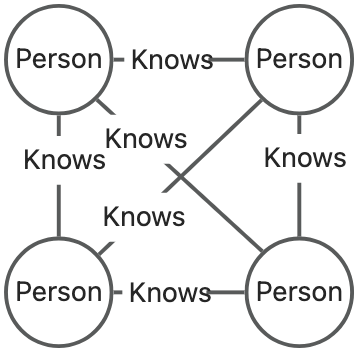
\includegraphics[width=.3\linewidth]{./figures/intro-pattern.png}
    \caption{Pattern graph corresponding to the conditions in the SQL query.}
    \label{fig:intro-pattern}
\end{figure}


Indeed, the conditions specified within this SQL statement collectively establish the structure of a pattern graph.
As shown in Fig.~\ref{fig:intro-pattern}, there are four vertices representing four persons, and these four persons form a complete graph.
Therefore, this SQL query can be expressed as a graph query.
The corresponding expression following the grammar of Cypher \cite{opencypher} is as follows:
\begin{lstlisting}
    MATCH (p1:Person)-[:Knows]-(p2:Person)-[:Knows]-(p3:Person)-[:Knows]-(p4:Person),
        (p1)-[:Knows]-(p3), (p2)-[:Knows]-(p4)
    RETURN p1.id, p2.id, p3.id, p4.id;
\end{lstlisting}
This graph query expression is much more concise and understandable than that in SQL.
It suggests that SQL is not always the optimal choice, and sometimes employing graph queries is more advantageous.
Then, in order to combine the extensive developments made in SQL queries over the years with the benefits of graph queries, it would be helpful for SQL to support both relational and graph queries.

Following this idea, the striking SQL/Property Graph Queries (abbr.~SQL/PGQ) is proposed.
In detail, SQL/PGQ is a part of SQL 2023 and its grammar allows to define and query graphs in SQL/PGQ expressions.
Consequently, some complex relational queries (such as those containing multiple joins) can be represented as relatively simple graph queries.
Specifically, graphs in SQL/PGQ are presented as views, and vertices and edges in the graphs are represented as tables.
It implies that with SQL/PGQ, graph queries and relational queries can be expressed in one statement and optimized together for a better execution plan.
An example of an SQL/PGQ query is provided in Example \ref{example:introduction:sqlpgq}.

\begin{example}
    \label{example:introduction:sqlpgq}
    Suppose three tables, i.e., \textbf{Person, Knows, Department}, are stored in the relational database.
    With SQL/PGQ, a graph view named \textbf{friendship\_graph} is created based on tables \textbf{Person} and \textbf{Knows}.
    Specifically, rows in table \textbf{Person} represent the vertices in the graph while rows in table \textbf{Knows} represent the edges.
    Besides, the department a person belonging to is stored in table \textbf{Person} as a foreign key (i.e., \textit{dept\_id}).

    Suppose we are going to find three persons satisfying: (1) They know each other; (2) Two of them belong to the Department of Computer Science.
    Then, the corresponding SQL/PGQ query is as follows:
    \begin{lstlisting}
        SELECT pn1, pn2, pn3
        FROM Department p, GRAPH_TABLE (friendship_graph
            MATCH (p1:Person)-[:Knows]-(p2:Person)-[:Knows]-(p3:Person),
            (p1)-[:Knows]-(p3)
            COLUMNS (
                p1.name as pn1,
                p1.dept_id as dept1,
                p2.name as pn2,
                p2.dept_id as dept2,
                p3.name as pn3,
                p3.dept_id as dept3)
        ) f
        WHERE dept1 = p.dept_id
        AND dept2 = p.dept_id AND
        AND p.dept_name = 'Computer Science';
    \end{lstlisting}
    According to the first condition, the obtained three persons should form a triangle.
    It is a problem of pattern matching, and such triangles are searched for on \textbf{friendship\_graph}.
    The output of the graph query is a table (named \textbf{f}) with six columns, i.e., pn1, dept1, pn2, dept2, pn3, and dept3, representing the names of the three persons and the identifiers of the departments they belonging to.

    For the second condition, due to the existence of the foreign key, it is efficient to perform natural join between table \textbf{f} and table \textbf{Department} to obtain the ideal results.
    Please note that the outputs of graph queries are still tables, and the outputs can be treated as tables within relational queries.
\end{example}

To support SQL/PGQ queries, it is more reasonable to enhance relational databases with the capability to process graph queries.
The reason is that relational databases have been widely utilized in both academia and industry, and it is costly and impractical to migrate data from relational databases to graph databases.
After the SQL/PGQ query is parsed, relational databases need to optimize the obtained abstract syntax tree (abbr.~AST).
However, since graph queries are allowed in SQL/PGQ queries, the existing relational databases can hardly optimize ASTs with graph operators.
Intuitively, there are some possible solutions, which can be mainly categorized into four types.
The stages of query optimization that these four types of solution are involved in respectively are shown in Fig.~\ref{fig:catagory}.

\begin{figure*}
    \centering
    \begin{subfigure}[b]{0.4\linewidth}
        \centering
        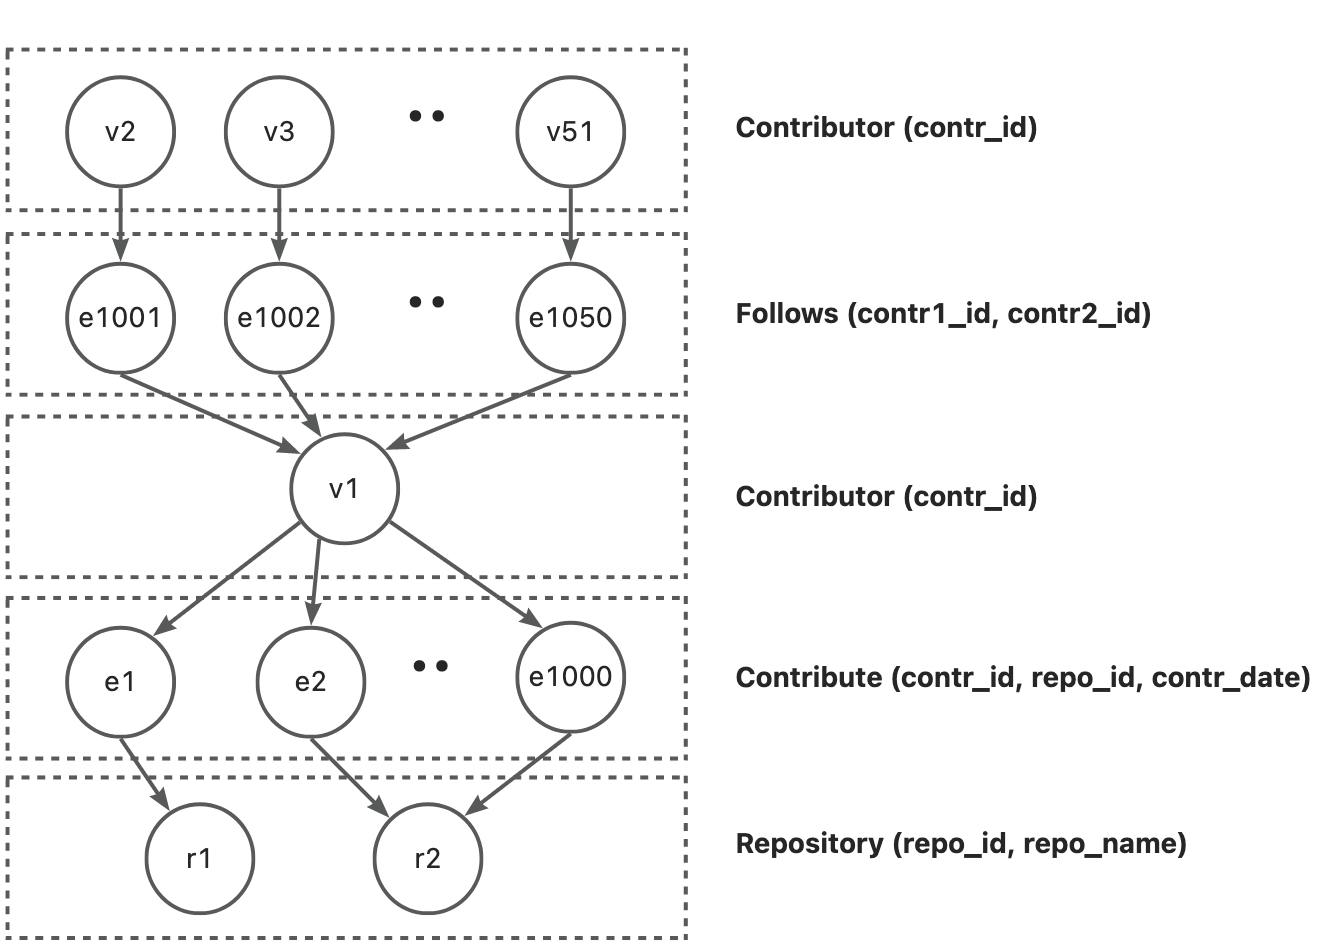
\includegraphics[width=\linewidth]{./figures/intro-order-case.png}
        \caption{Relationship 1.}
        \label{fig:intro-order-case}
    \end{subfigure}
    \begin{subfigure}[b]{0.4\linewidth}
        \centering
        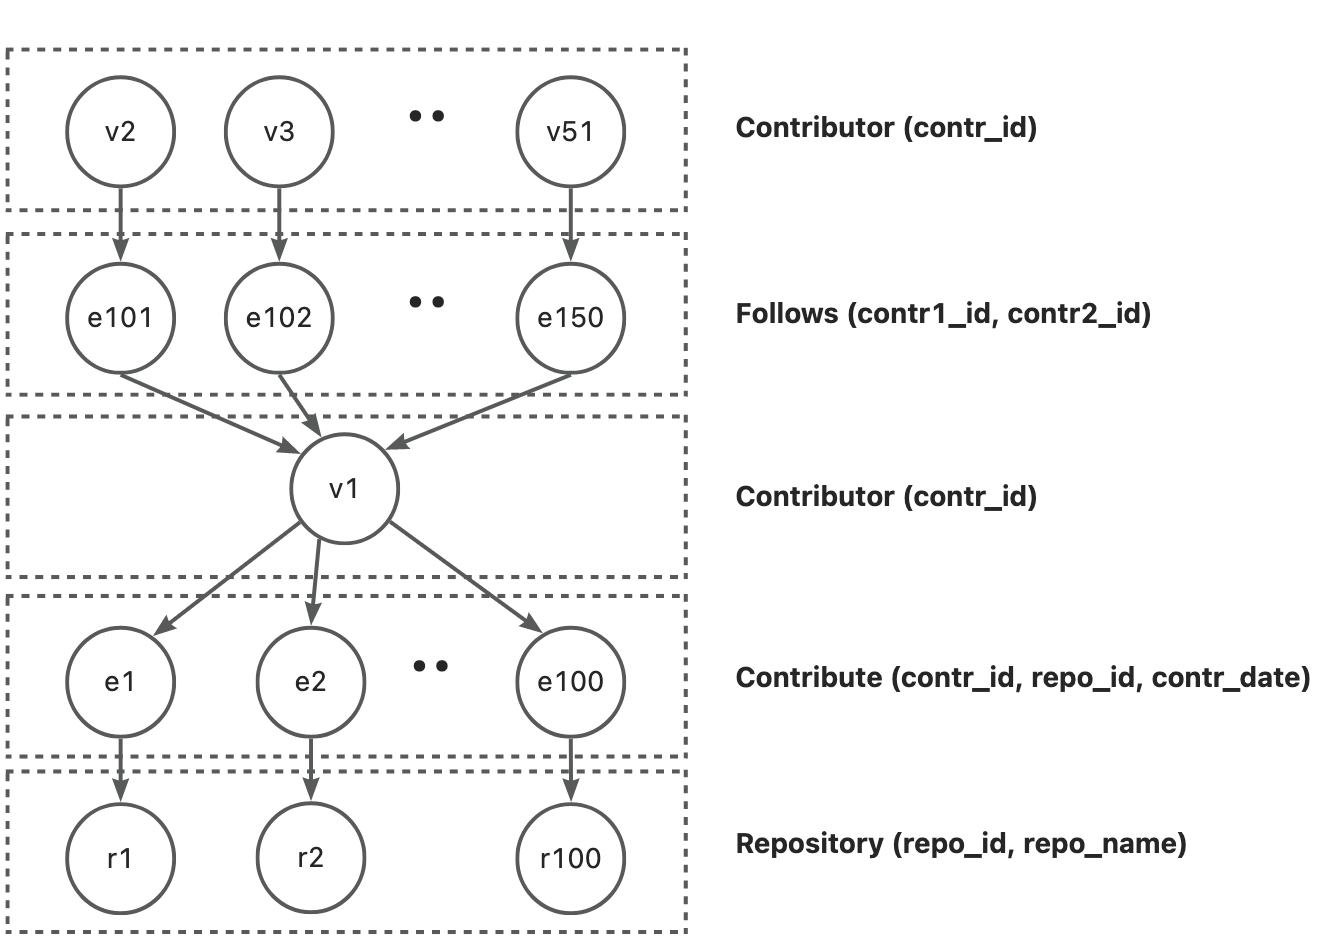
\includegraphics[width=\linewidth]{./figures/intro-order-case-2.png}
        \caption{Relationship 2.}
        \label{fig:intro-order-case2}
    \end{subfigure}
    \caption{Graphs representing the relationships among tuples in different tables. In detail, tuples in Tables \textbf{Contributor} and \textbf{Repository} represent vertices in the graph, while those in Tables \textbf{Follows} and \textbf{Contirbute} represent edges.}
    \label{fig:intro-replace-example}
\end{figure*}

\begin{figure*}
    \centering
    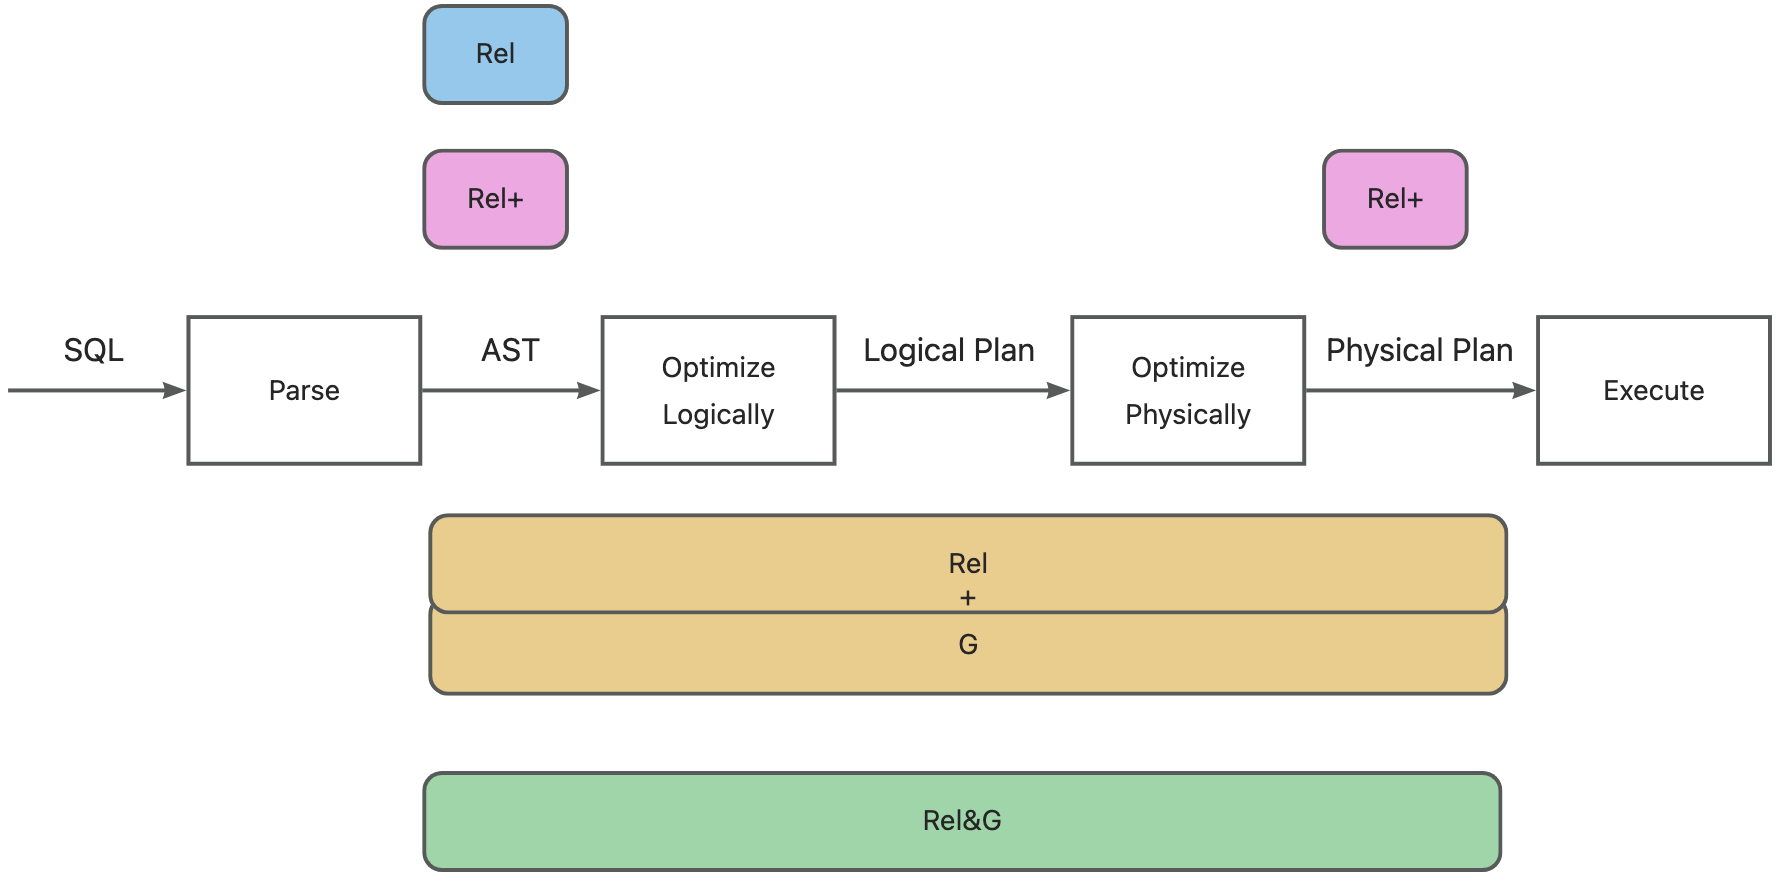
\includegraphics[width=.6\linewidth]{./figures/catagory.png}
    \caption{The stages of query optimization that the four kinds of solutions are involved in.}
    \label{fig:catagory}
\end{figure*}

\textbf{Solution 1 ($Rel$)}.
The most direct solution is to transform graph queries to relational ones, and then optimize the new queries with relational optimizers.
Apache Age \cite{apache-age} and DuckPGQ \cite{DuckPGQ,DuckPGQ-VLDB} are typical examples.
However, methods of this type only take effect in the stage of logical optimization and degrade into relational optimizers.
Therefore, they lose the chance of query optimization from the graph perspecitve.

\begin{example}
    Given four tables \textbf{Contributor}, \textbf{Follows}, \textbf{Contribute}, and \textbf{Repository} as shown in Fig.~\ref{fig:intro-order-case}, the relationships among their tuples are presented.
    Specifically, edge (v1, e1) means that e1.contr\_id = v1.contr\_id and edge (e1, r1) means that e1.repo\_id = r1.repo\_id.
    Moreover, suppose graph indices have been built on tables \textbf{Follows} and \textbf{Contribute}.
    Then, given a contributor, the followers of the contributor and the repositories the contributor contributes to can be directly retrieved with the indices, respectively.

    Suppose we are going to find the followers of $v1$, and the query is as follows:
    \begin{lstlisting}
        SELECT pid
        FROM GRAPH_TABLE (graph_view
            MATCH (p1:Contributor)-[:Follows]->(p2:Contributor {id: 1})
            COLUMNS (p1.id as pid)
        );
    \end{lstlisting}
    If the graph query is transformed to the corresponding relational query, then the followers of $v1$ can only be found with a join between \textbf{Contributor} and \textbf{Follows}, and another join between the resultant table and \textbf{Contributor}.
    In this process, the graph indices cannot be utilized, and the process is far from efficient.
\end{example}


\textbf{Solution 2 ($Rel^+$)}.
Methods of this type build graph indices on relational databases and introduce new operators to perform graph queries based on the indices.
However, these new operators are applied after the optimial physical plan is obtained with the relational optimizer.
As shown in Fig.~\ref{fig:catagory}, such methods are separately involved in the stages of logical optimization and physical optimization.
It means that the optimizations w.r.t.~graph operators at the logical layer and the physical layer are disjointed.
To be more specific, the cost of new operators introduced in physical optimization are unawared in logical optimization.

The optimizer in GrainDB \cite{graindb} is a representative of type $Rel^+$.
GrainDB builds RID indices on DuckDB \cite{duckdb}, and proposes two new join methods, i.e., sip-join and merge-sip-join.
In detail, sip-join gets adjacent edges of vertices or gets adjacent vertices of edges based on the RID indices, while merge-sip-join obtains the neighbors of vertices.
Since GrainDB follows the grammar of SQL, given a SQL/PGQ query, the query is transformed to the equal relational query frist, and then GrainDB optimizes the query with the relational optimizer of DuckDB to obtain the optimal execution plan.
Next, GrainDB replaces some hash-joins in the plan with sip-joins and merge-sip-joins to leverage the graph indices.
It indicates that the cost-based optimization in GrainDB only finds the optimal execution plan before the graph indices are awared.
Therefore, the plan can be suboptimal after replacement.
Moreover, some efficient replacement cannot be applied w.r.t.~the obtained execution plan due to the order of joining tables representing vertices and edges.
An example is shown as follows.

\begin{example}
    Given four tables as shown in Fig.~\ref{fig:intro-order-case}, a SQL/PGQ query is as follows:
    \begin{lstlisting}
        SELECT contr_id, repo_name
        FROM GRAPH_TABLE (graph_view
            MATCH (p2:Contributor)-[f:Follows]->(p1:Contributor {contr_id: 1})-[c:Contribute]->(r:Repository)
            COLUMNS (p2.contr_id as contr_id,
                    r.repo_name as repo_name)
        );
    \end{lstlisting}
    %\begin{lstlisting}
    %    SELECT p2.contr_id, repo_name
    %    FROM Contributor p1, Follows f, Contributor p2, Contribute c, Repository p
    %    WHERE p1.contr_id = 1
    %    AND p1.contr_id = f.contr2_id
    %    AND p2.contr_id = f.contr1_id
    %    AND p1.contr_id = c.contr_id
    %    AND c.repo_id = r.repo_id;
    %\end{lstlisting}
    From the perspecitve of a relational database (e.g., DuckDB), the best join order can be \textbf{p1$\rightarrow$f$\rightarrow$p2$\rightarrow$c$\rightarrow$r}, since tables \textbf{Follows} and \textbf{Contributor} have much smaller cardinalities than table \textbf{Contribute}.
    Then, by replacing the join operators with getNeighbor, the finally obtained execution plan is \textbf{p1$\xrightarrow{\textit{getNeighbor}}$p2$\xrightarrow{\textit{getNeighbor}}$r}.

    However, as $v_1$ has much fewer neighbors in table \textbf{Repository} than in table \textbf{Contributor}, join order \textbf{p1$\xrightarrow{\textit{getNeighbor}}$r$\xrightarrow{\textit{getNeighbor}}$p2} would be more efficient from the perspective of graph databases.
    Therefore, it suggests that
    replacing relational operators with graph operators after optimization with relational optimizers can miss optimial execution plans.

    Besides, given the relationships among the tuples as shown in Fig.~\ref{fig:intro-order-case2}, the best join order from the perspective of a relational database like DuckDB can be \textbf{p1$\rightarrow$f$\rightarrow$c$\rightarrow$p2$\rightarrow$r}.
    Then, \textbf{p1$\rightarrow$f} and \textbf{c$\rightarrow$p2} cannot be replaced with \textbf{p1$\xrightarrow{\textit{getNeighbor}}$p2} and some efficient execution plans are missing.

    %An example about replace join with getV/getE/getNeighbor,
    %or the example of duckdb, whether to indicate more constraints (due to the unawareness of getNeighbor)
\end{example}


\textbf{Solution 3 ($Rel+G$)}.
According to the grammar of SQL/PGQ, the graph queries usually starts with keyword GRAPH\_TABLE.
Therefore, graph queries can be easily distinguished in SQL/PGQ queries.
Hence, it is possible to optimize graph queries first with graph optimizers, and then optimize the relational query with relational optimizers.
As shown in Fig.~\ref{fig:catagory}, the logical and physical optimization are related, and the cost of graph operators are estimated in the process of optimization.
However, this solution still has limitations, e.g., graph queries and relational queries are optimized separately, and cross-queries optimizations are missing.
An example about this limitation is presented.

\begin{example}
    \label{example:push_down}
    Suppose we are going to find persons that know John and the query expression is as follows:
    \begin{lstlisting}
        SELECT p FROM GRAPH_TABLE (friendship_graph
            MATCH (p1:Person)-[:Knows]-(p2:Person)
            COLUMNS (p1.name as p, p2.name as p2)
        )
        WHERE p2 = 'John';
    \end{lstlisting}
    For $Rel+G$ methods, the graph query is first optimized with a graph optimizer, and the optimized plan finds all pairs of persons that know each other.
    Then, the relational optimizer optimizes the relational query, which finds the persons that know John.
    Please note that the condition ``p2 = 'John''' in the relational query can be pushed down into the graph query, so that the graph query only returns persons that know John.
    The optimized query is as follows.
    \begin{lstlisting}
        SELECT p FROM GRAPH_TABLE (friendship_graph
            MATCH (p1:Person)-[:Knows]-(p2:Person {name: 'John'})
            COLUMNS (p1.name as p)
        );
    \end{lstlisting}
    However, since $Rel+G$ methods optimize relational queries and graph queries separately and do not apply cross-queries optimizations, the condition cannot be pushed down and the optimal execution plan is missed.
\end{example}

In this paper, we propose \textbf{Solution 4 ($Rel\&G$)}, which optimizes the graph queries and relational queries simultaneously with cross-queries optimizations.
Such a solution can fully leverage the advantages of both relational optimizers and graph optimizers.
In detail, we propose a new converged optimization framework of this type for SQL/PGQ.
The framework first generates the converged logical plan consisting of a relational subplan and several graph subplans.
Then, optimization strategies including CBOs and RBOs are applied to optimize inside and crossing subplans.
The contributions of this paper are mainly as follows:

(1) To the best of our knowledge, this is the first optimization framework for SQL/PGQ query optimization.
Property graphs are represented as views in SQL/PGQ, and vertices and edges are associated with tables in the relational databases.
Then, it is crucial to offer a converged query optimizer efficient for SQL/PGQ queries to optimize both relational and graph queries in SQL/PGQ statements.

(2) The framework proposes a new Scan operator named ScanGraphTable to retrieve data from graph tables obtained with graph queries.
The output of ScanGraphTable is a relational table and it bridges the gap between graph subplans and relational subplans.

(3) We prove that graph pattern matching expressed in graph queries of SQL/PGQ can be expressed with graph relational algebra, which confirms that the converged graph relational optimization framework can optimize SQL/PGQ queries and obtain correct results.


% In the framework, we design and implement numerous important operators for graph optimizer, including getV, getE, getNeighbor, and extendIntersect.
% Specifically, the extendIntersect operator is helpful in supporting worst-case optimality.

(4) Theoretical analysis on the complexity of the optimization framework is conducted.
The obtained theorems prove that for graph queries, the join order optimization with a graph optimizer can be exponentially faster than that with a relational optimizer.
It theoretically confirms that relational optimizer is usually not suitable for graph queries, and it is indispensable for the existence of a converged optimization framework.

(5) Extensive experiments are conducted to show the efficiency of the proposed converged query optimization framework.
The experimental results show that the framework can be ?$\times$ faster than the baselines.

The rest of this paper is organized as follows.


The existing methods for optimizing the SPJM queries can be divided into four categories.
The main difference between these methods lies in the approach to handling the matching operator.
Before the details of these methods are introduced, concepts about graph structure and graph matching decomposition are proposed as follows.
}

\section{Preliminaries}
\label{sec:preliminaries}

\subsection{Data Model}
\label{sec:data-model}

A schema, denoted as \(S = (a_1, a_2, \ldots, a_n)\), is a collection of attributes. Each attribute \(a_i\) in this schema is associated with a specific data domain \(D_i\), which defines the set of permissible values that \(a_i\) can take.
A relation \(R\) is defined as a set of tuples. We consider \(R\) to be a relation over schema \(S\), if and only if, every tuple \(\tau = (d_1, d_2, \ldots, d_n)\) in \(R\) adheres to the schema's constraints, such that the value \(d_i\) for each position in the tuple corresponds to the data domain \(D_i\) of the attribute \(a_i\) in \(S\). In other words, each value \(d_i\) in a tuple \(\tau\) is drawn from the appropriate data domain \(D_i\) for its corresponding attribute \(a_i\).
Moreover, for any tuple \(\tau\) in the relation \(R\), the notation \(\tau.a_i = d_i\) signifies that the attribute \(a_i\) in tuple \(\tau\) has the value \(d_i\). A table is a representation of a relation, where each row corresponds to a tuple in the relation, and each column represents an attribute in the schema. In this paper, we use the terms of relation and table interchangeably.

We define a \emph{Property Graph} as $G = (V_G, E_G)$,
where
\begin{itemize}
    \item $V$ stands for the set of vertices.
    \item Let $E \subseteq V \times V$ denote the set of edges in the graph. An edge $e \in E$ is represented as an ordered pair $e = (v_s, v_t)$, where $v_s \in V$ is the source vertex and $v_t \in V$ is the target vertex, indicating that the edge $e$ connects from $v_s$ to $v_t$.
    %we use $\id(e)$ and $\lab(e)$ to denote the globally unique id and label of $e$, and $\attr(e, a_i)$, or $e.a_i$, to denote the value of the attribute $a_i$ of $e$.
    \item For any graph element $\epsilon$ that is either a vertex or an edge, we denote $\id(\epsilon)$ and $\lab(\epsilon)$ as the globally unique ID and the label of $\epsilon$, respectively. Given an attribute $a_i$, $\epsilon.a_i$ denotes the value of the attribute $a$ of $\epsilon$.
\end{itemize}


Given a vertex $v$, we denote its adjacent edges as $\adj_G^E(v) = \{e = (v, v_t) | e \in E\}$ and its adjacent vertices (i.e., neighbors) as $\adj_G(v) = \{v_t | (v, v_t) \in E\}$\footnote{It is important to note that the adjacent edges and vertices can be defined for both directions of an edge $e = (v_s, v_t)$, i.e., when $v = v_s$ or $v = v_t$. However, for simplicity, we only define one direction in this notation. In the actual semantics of the paper, both directions may be considered.}. The degree of $v$ is defined as $d_G(v) = |\adj_G(v)|$, and the average degree of all vertices in the graph is $\overline{d}_G = \frac{1}{|V_G|} \sum_{v \in V_G} d_G(v)$.
In the rest of the paper, when the context is clear, we may remove $G$ from the subscript for simplicity, for example $G=(V, E)$.

Considering two graphs \(G_1\) and \(G_2\), we assert that \(G_2\) is a subgraph of \(G_1\), symbolized as \(G_2 \subseteq G_1\), if and only if \(V_{G_2} \subseteq V_{G_1}\), and \(E_{G_2} \subseteq (E_{G_1}\)). Furthermore, \(G_2\) qualifies as an induced subgraph of \(G_1\) under the condition that \(G_2\) is already a subgraph of \(G_1\), and for every pair of vertices in \(G_2\), any edge \(e\) that exists between them in \(G_1\) must also present in \(G_2\).

To formalize the integration of graph syntax within the realm of relational data, we introduce the concept of a \textit{Relations-to-Graph Mapping} (i.e. \rgmapping), to facilitate the transformation of relational data structures into a property graph.

%Given two relations, \(R_1\) and \(R_2\), each with its own schema. Let there be a bijective relation mapping, \(\lambda: R_1 \mapsto R_2 \).
\begin{definition}[\rgmapping]
\label{def:rgmapping}
Given two set of relations $\{R_{p_1}, \ldots, R_{p_n}\}$ and $\{R_{q_1}, \ldots, R_{q_m}\}$,
we define an \rgmapping to map the relations to a property graph $G = (V, E)$, %which contains the mappings of $(\zeta_v, \zeta_e, \lambda_{e_1}^s, \lambda_{e_1}^t, \ldots, \lambda_{e_m}^s, \lambda_{e_m}^t)$,
which are elaborated as follows:

\begin{itemize}
\item \textbf{Vertex Mappings}: $\zeta_v: \bigcup_{i=1}^{n} R_{p_i} \mapsto V$ is a bijective function that maps every tuple $\tau \in R_{v_i}$ for all $1 \leq i \leq n$ to a unique vertex $v \in V$. This vertex $v$ is assigned: an ID $\id(v)$, a label $\lab(v)$ that matches the name of $R_{v_i}$, and attributes $v.attr*$ that mirror the attributes $attr*$ of $\tau$.
The relations that are mapped to vertices in the graph are referred to as vertex relations.

\item \textbf{Edge Mappings}: $\zeta_e: \bigcup_{i=1}^{m} R_{q_i} \mapsto E$ is a bijective function that maps every tuple $\tau \in R_{q_i}$ for all $1 \leq i \leq m$ to a unique edge $e = (v_s, v_t) \in E$. Similar to vertices, each edge $e$ is assigned: an ID $\id(e)$,
a label $\lab(e)$ corresponding to the name of $R_{q_i}$, and attributes $e.attr*$ that reflect the attributes $\tau.attr*$ of $\tau$.
For each edge relation $R_{q_i}$, there are two corresponding vertex relations $R_{p_s}$ and $R_{p_t}$.
We further define two total functions: $\lambda_{q_i}^s: R_{q_i} \to R_{p_s}$ and $\lambda_{q_i}^t: R_{q_i} \to R_{p_t}$, which maps a tuple $\tau \in R_{q_i}$ to a tuple $\tau_s \in R_{p_s}$ and a tuple $\tau_t \in R_{p_t}$, respectively.
The vertices $v_s$ and $v_t$ corresponding to $\tau_s$ and $\tau_t$, respectively, are obtained by applying the vertex mapping function $\zeta_v$, i.e., $v_s = \zeta_v(\tau_s)$ and $v_t = \zeta_v(\tau_t)$.
The relations $R_{q_i}$ that are mapped to edges in the graph are referred to as edge relations.
\end{itemize}
\end{definition}

\begin{figure*}
    \centering
    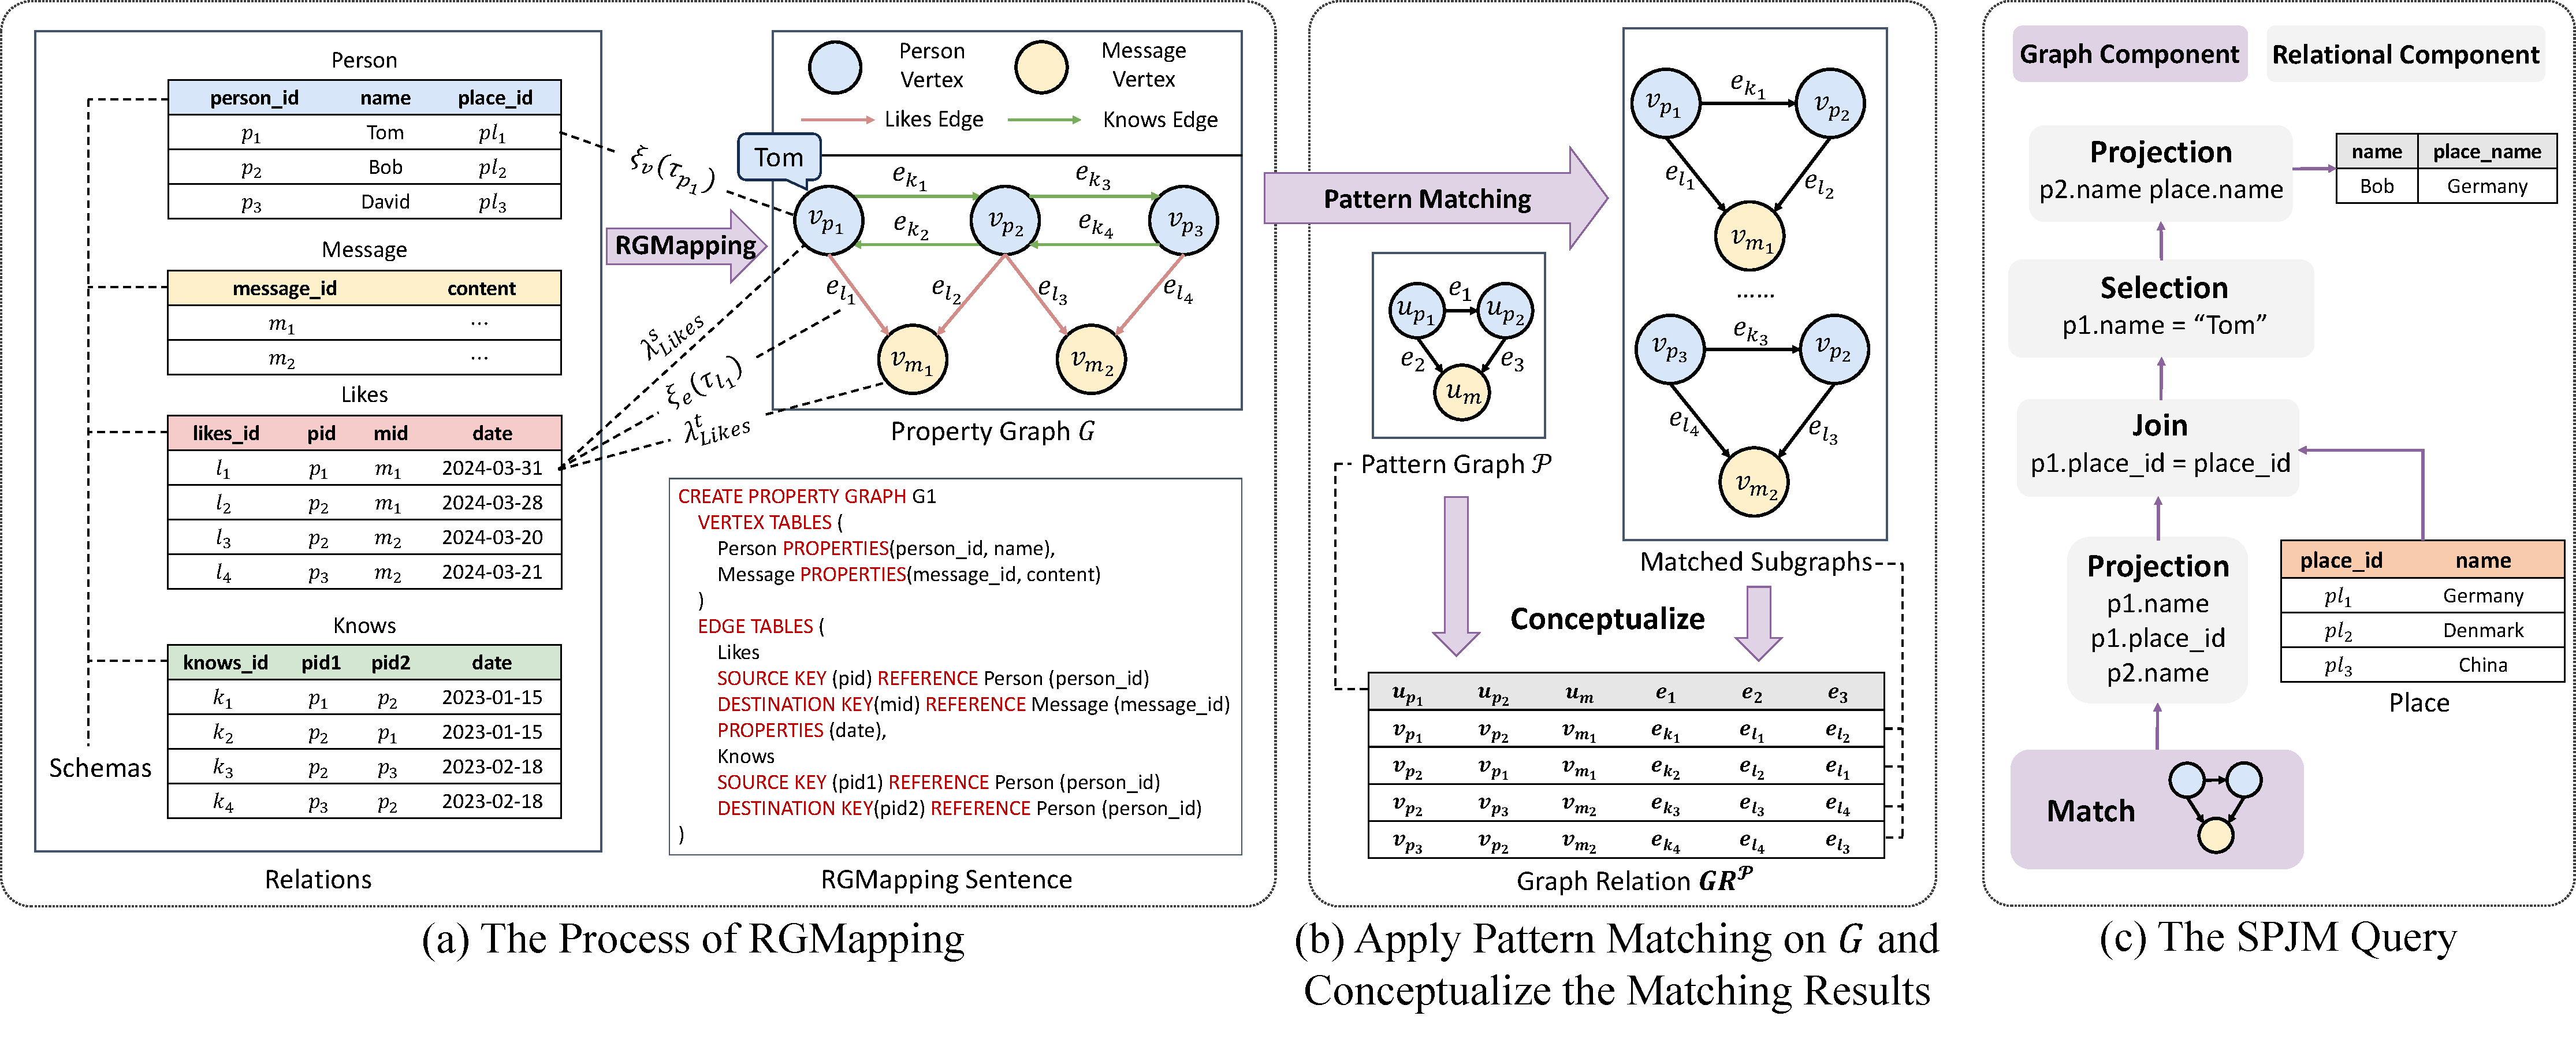
\includegraphics[width=\linewidth]{./figures/rgmapping.pdf}
    \caption{An example of \rgmapping.}
    \label{fig:intro-rgmapping-example}
\end{figure*}

\begin{example}
    \label{ex:rgmapping}
    An \rgmapping can be defined following the grammar of SQL/PGQ with \lstinline{CREATE PROPERTY GRAPH} statements.
    Given five relations, an \rgmapping is defined with the statement shown in Fig.~\ref{fig:intro-rgmapping-example}(a).
    \iffalse
    \begin{equation*}
        \begin{split}
            & \textit{Person = (\underline{person\_id}, name, place\_id)} \\
            & \textit{Message = (\underline{message\_id}, content)} \\
            & \textit{Place = (\underline{place\_id}, pl\_name)} \\
            & \textit{Likes = (\underline{likes\_id}, pid, mid, date)} \\
            & \textit{Knows = (\underline{knows\_id}, pid1, pid2, date)}
        \end{split}
    \end{equation*}
    \fi
    %the following statement defines an \rgmapping (\todo{better plot the statement in Figure 4}):
    \iffalse
    \begin{lstlisting}
CREATE PROPERTY GRAPH G1
    VERTEX TABLES (
       Person PROPERTIES(person_id, name),
       Message PROPERTIES(message_id, content)
    )
    EDGE TABLES (
       Likes
       SOURCE KEY(pid) REFERENCE Person(person_id)
       DESTINATION KEY(mid) REFERENCE Message(message_id)
       PROPERTIES(date),
       Knows
       SOURCE KEY(pid1) REFERENCE Person(person_id)
       DESTINATION KEY(pid2) REFERENCE Person(person_id)
    )
    \end{lstlisting}
    \fi
    The described \rgmapping involves assigning tuples from vertex relations, such as $\relation{Person}$ and $\relation{Message}$, to graph vertices. For instance, the vertex $v_{p_1}$ is associated with the tuple $\tau_{p_1}$ in $\relation{Person}$, and thus assigned the label ``Person'' and the name attribute ``Tom''. Similarly, edge relations $\relation{Likes}$ and $\relation{Knows}$ correspond to graph edges.
    To further elaborate on the mapping process, especially for the source and target vertex mappings of an edge, let's consider the edge $e_{l_1}$. This edge originates from the tuple $\tau_{l_1}$ in the $\relation{Likes}$ relation. The source vertex $v_{p_1}$ of $e_{l_1}$ is linked to the tuple $\tau_{p_1}$ in $\relation{Person}$ via the function $\lambda_{Likes}^s$, following the condition ``$\tau_{l_1}.pid = \tau_{p_1}.\text{person\_id}$''. Similarly, the target vertex $v_{m_1}$ is associated with the tuple $\tau_{m_1}$ in $\relation{Message}$ via the function $\lambda_{Likes}^t$, following the condition ``$\tau_{l_1}.mid = \tau_{m_1}.\text{message\_id}$''. As a result of this mapping, the edge $e_{l_1}$ is assigned the label ``Likes'' and the attribute ``date'' with the value ``2024-03-31''.
\end{example}

%In the rest of this paper, let $\mathcal{J}_{GR} = 2^{2^{V \cup E}}$ be the domain of graph relations, $\mathcal{J}_R = 2^{2^{D}}$ be the domain of relations, and $\mathcal{J} = \mathcal{J}_{GR} \cup \mathcal{J}_R$.

\subsection{Matching Operator}
\label{sec:matching-operator}
Consider a property graph \(G(V_G, E_G)\), alongside a \emph{connected} pattern graph, represented as \(\pattern(V_\pattern, E_\pattern)\). Here, \(\pattern\) is a property graph that does not possess attributes, and
we denote $n$ and $m$ as the number of vertices and edges in the $\pattern$, respectively.
%Graph pattern matching is defined as the task of identifying all subgraphs within a target graph \(G\) that are \emph{homomorphic} to \(\pattern\).
Graph pattern matching seeks to determine all subgraphs in \(G\) that are \emph{homomorphic} to \(\pattern\).
Formally, given a subgraph $g \subseteq G$, a homomorphism from \(\pattern\) to \(g\) is a \emph{surjective}, total mapping \(f: V_\pattern \cup E_\pattern \to V_{g} \cup E_{g}\) that satisfies the following conditions: (1) For every vertex \(u \in V_\pattern\), there is a corresponding vertex \(v = f(u) \in V_{g}\) with \(\lab(v) = \lab(u)\)\footnote{As a convention, we will always write $u$ and $v$ for a pattern vertex and a graph vertex, respectively.}; (2) For each edge \(e = (u_s, u_t) \in E_\pattern\), there is a corresponding edge \(f(e) = (v_s, v_t) \in E_{g}\), ensuring that the mapping preserves the edge's the label, as well as its source and target vertices , that is \(\lab(e) = \lab(f(e))\), and \(f(u_s) = v_s\), \(f(u_t) = v_t\). It's important to highlight the homomorphism semantics, as one of the widely used semantics for graph pattern matching~\cite{angles2017foundations}, \modify{does} not require each pattern vertex and edge being uniquely mapped to distinct vertices and edges in the data graph. This facilitates a seamless integration between graph pattern matching and relational operations, but alternative semantics for graph pattern matching such as isomorphism can also be adopted, as will be further discussed in~\refsec{handling-match-operator}.

The outcomes of graph pattern matching can be succinctly modeled as a relation \(GR_G^\pattern\), or more compactly \(GR^\pattern\) in clear contexts, defined over the schema \(S = V_\pattern \cup E_\pattern\). Here, the sets \(V_G\) and \(E_G\) serve as the respective domains for the vertices and edges identified through the matching process. Within this framework, we refer to such a relation as a \emph{Graph Relation}, a construct where all attributes are derived from the domain of a property graph.
It is essential to recognize that any property graph \(G\) can be conceptualized as a graph relation \(GR^G\), represented by a singular tuple that collectively encompasses all of its vertices and edges. Throughout this paper, we treat the notions of a property graph and a tuple of graph relation as essentially interchangeable terms. In alignment with this perspective, we proceed to elaborate on the \emph{Matching} operator as follows.

%The formulation of graph relation inherently positions any graph $G$ as a graph relation consisting of a single tuple that encapsulates the entirety of its vertices and edges.
%he results of graph pattern matching can be represented as a relation \(R_G(\pattern)\) (or \(GR(\pattern)\) for short when the context is clear) over the schema  \(S = V_\pattern \cup E_\pattern\), wherein \(V_G\) and \(E_G\) act as the domains for the vertices and edges that have been matched, respectively. In this paper, we call such a relation a \emph{graph relation}, when all attributes of the relation are from the domain of a property graph.
%It's clear that any graph $G$ can be represented as a graph relation consisting of a single tuple that encapsulates the entirety of its vertices and edges. In this paper, the concepts of property graph and graph relation can always be used interchangeably. In this context, we introduce the \emph{Match} operator as detailed below.

%likewise expressible as a graph relation \(GR_G(\pattern)\) (or \(GR(\pattern)\) for short when the context is clear) based on the schema \(S = V_\pattern \cup E_\pattern\), wherein \(V_G\) and \(E_G\) act as the domains for the vertices and edges that have been matched, respectively. In this context, we introduce the \emph{Match} operator as detailed below.

\begin{definition}[Matching Operator, \(\matching\)]
    \label{def:matching}
    The Matching Operator, denoted as \(\matching\), is designed to perform graph pattern matching on a given graph relation \(GR\) against a specified pattern graph \(\pattern\). For each graph instance \(g\) within \(GR\), \(\matching\) identifies all subgraphs of \(g\) that are homomorphic to \(\pattern\), and subsequently, aggregates these mappings to construct a comprehensive graph relation. The operation of the matching Operator can be formally articulated as \(\matching(GR, \pattern) = \bigcup_{g \in GR} GR_g^\pattern\).%, where each \(GR_g^\pattern\) represents the subgraph(s) of \(g\) that align with the structure and properties of \(\pattern\).
\end{definition}

\begin{example}
    \label{ex:matching}
    Let \(G_1\) denote the property graph derived from the relations via \rgmapping in \refex{rgmapping}.
    Given a pattern graph \(\pattern\) shown in \reffig{intro-rgmapping-example}(b), the results of graph pattern matching are subgraphs of \(G_1\) that are homomorphic to \(\pattern\), which are represented as a graph relation \(GR^\pattern = \matching(GR^{G_1}, \pattern)\), wherein each tuple corresponds to one of the matched subgraph.
\end{example}

This definition ensures that the matching operator is inherently closed regarding graph relations,
which adheres to the language opportunities of ``nested matching'' (specified as PGQ-079) in SQL/PGQ~\cite{sql-pgq}.
In this paper, we only handle cases where $G$ represents the entire property graph, and thereafter simplify the matching operator notation to $\matching(\pattern)$ when the context is clear.

\subsection{Problem Definition}
\label{sec:problem-definition}

To study relational query optimization, it is common to focus on a category of queries known as \spj queries,
which encapsulate the three most frequently employed operations in database management: select, project, and (natural) join.
These operations form the backbone of many relational queries. Given a set of relations \(R_1, R_2, \ldots, R_m\),
an \spj query is formally represented as:
\[
Q = \pi_A(\sigma_\Omega(R_1 \Join \cdots \Join R_m)).
\]

Inspired from the \spj paradigm, we introduce a novel category of queries, termed \spjm queries, to logically formulate SQL/PGQ~\cite{sql-pgq} queries that
blend relational and graph operations. Our focus is not on an exhaustive exploration of SQL/PGQ, which encompasses a broad spectrum of operations, but rather on understanding and enhancing the core functional elements of such queries.
The \spjm framework augments \spj queries by incorporating a matching operator, thereby enriching the query's expressive power to seamlessly navigate both relational and graph data domains.
Given the set of relations and a property graph \(G\) constructed from these relations via an \rgmapping (\refdef{rgmapping}),
an \spjm query is articulated as:

\begin{equation}
    \label{eq:spjm}
Q = \pi_A(\sigma_\Omega(R_1 \Join \cdots \Join R_m \Join (\widehat{\pi}_{A*}\matching_G(\pattern))))
\end{equation}
In this formulation, \(\widehat{\pi}_{A*}\matching_G(\pattern)\) is the \emph{graph component} of
the query, while the remaining part of the query is an \spj expression referred to as the \emph{relational component}.
Here, \(\matching_G(\pattern)\) represents the process of matching the pattern \(\pattern\) on the graph \(G\) and
returns a graph relation as defined in \refdef{matching}. The operator \(\widehat{\pi}_{A*}\) is a
graph-calibrated projection operator that extracts the ID, label, and other attributes from the vertices and edges in the matched results.
This process helps ``flatten'' graph elements into relational tuples.
For example, given a graph relation $GR$ that contains a vertex of \{ID:0, label:Person, name:``Tom''\}, the
following projection
\[
\widehat{\pi}_{\id(v) \rightarrow \text{v\_id}, \lab(v) \rightarrow \text{v\_label}, v.name \rightarrow \text{v\_name}}(GR)
\]
turns the vertex into a relational tuple of (0, Person, ``Tom'').
The projection operation is designed to reflect the \lstinline{COLUMNS} clause in SQL/PGQ
to retrieve specific attributes from vertices and edges as required. For simplicity, we assume that all
attributes are extracted unless otherwise specified.

In this paper, we study the problem of optimizing \spjm queries in \refeq{spjm}.

\begin{example}
    \reffig{intro-rgmapping-example}(c) illustrates an example of an \spjm query, along with its corresponding SQL/PGQ expression. The query's objective is to identify pairs of persons who like the same message, know each other, and where one of them resides in Germany. As per the query, once the results of the matching operator are obtained (as described in \refex{matching}), a $\gproject$ operator is applied to extract attributes from all vertices, forming a relational table. Subsequently, the join, selection, and projection operators are employed to compute the final results.
    %Specifically, Tom, who is German, and Bob know each other and like the same message $m_1$.
\end{example}

\reftable{notations} summarizes frequently used notations in this paper.
\begin{table}[ht]
    \centering
   \caption{Frequently used notations.}
   \label{tab:notations}
    \scalebox{0.9}{
        \begin{tabular}{|m{0.34\linewidth}|m{0.63\linewidth}|}
            \hline
            Notation                 & Definition                                                                                       \\
            \hline
            $R$    & a relation or relational table   \\
            \hline
            $\tau$ and $\tau.attr$    & a tuple in a relation, and the value of an attribute of $\tau$ \\
            \hline
            $G(V,E)$         & a property graph with $V$ and $E$                                                          \\
            \hline
            $\pattern(V, E)$   & a pattern graph with $V$ and $E$  \\
            \hline
            $\id(\epsilon)$, $\lab(\epsilon)$, $\epsilon$.attr  & the identifier, label, and the value of given attribute of a graph element $\epsilon$ \\
            \hline
            $\adj(u)$ and $\adj^E(u)$           & neighbors and adjacent edges of $u$           \\
            \hline
            $GR$   & a graph relation     \\
            \hline
            $\matching(GR, \pattern)$, $\matching(\pattern)$  & matching $\pattern$ on a graph relation $GR$ or a graph $G$ \\
            \hline
            $\pi_{A}$, $\sigma_\Omega$, $\Join$  & projection, selection, and join operators over relations \\
            \hline
            $\gproject$, $\gjoin$  & projection and join operators over graph relations \\
            \hline
            $\lambda^s_\lab(e)$, $\lambda^t_\lab(e)$  & the total functions for mapping tuples in an edge relation to source and target vertex relations \\
            \hline
        \end{tabular}
    }
    % \vspace{-.05in}
\end{table}

%is a relation generated by projecting the outputs of the matching operator $\mathcal{M}$ to relations of properties.
%Besides, $GR_i$ is the graph relation that contains the data graphs that pattern matching is conducted on and $\mathcal{P}_i$ is the pattern.
%$prop_i$ is a list of necessary properties of vertices and edges in the resultant relation.

\iffalse
Regarding the SPJM problem, the main difference between the aforementioned four types of optimizers lies in their search space when optimizing the physical implementation of the matching operator.
Specifically, for $Rel$ methods, the matching operator is implemented with only joins that do not leverage graph indices (named relational joins) such as hash joins.
Therefore, $\widetilde{R}_i$ can be optimized with the relational optimizer.
For $Rel^+$ methods, in the process of optimization, the matching operator is implemented with relational joins.
Thus, the relational optimizer is also utilized to optimize $\widetilde{R_i}$.
However, after that, relational joins are replaced with joins that leverage graph indices (named graph joins) if possible such as sip join in GrainDB.
For $Rel+G$ methods, graph joins are considered in implementing the matching operator.
Then, operators inside of $\widetilde{R}_i$ are optimized by the graph optimizer, while the operators out of $\widetilde{R}_i$ are optimized by the relational optimizer.
Besides, the optimizations cannot be simultaneously related to operators within and outside of $\widetilde{R}_i$.
For example, the filter operators, i.e., $\sigma_d$ cannot be pushed into $\widetilde{R}_i$.
For $Rel\&G$, such optimizations are allowed.
\fi

% The search space for relgo in the context of a SPJG query consists of operator trees that correspond to sequence of join operators, e.g., the sequence
% \begin{lstlisting}
%     Join(Join(Join(Join(GR_1, GR_2), R_1), R_2), R_3)
% \end{lstlisting}


\iffalse
\subsection{Equivalence Between Graph Pattern Matching and Graph Relational Operators}
\label{sec:proof-gpm-gro}

For the SPJG problem to be solved in this paper, we need to obtain the graph relations by pattern matching.
In detail, the pattern matching process ought to be expressible through the traversal of paths, which are sequences of source, expand, and join operators.
In this section, we prove that the matching operator can be replaced with source, expand, and join operators. without changing the semantics of the query.
Then, the matching order can be further optimized by relgo.

We start from the case that there is only one path in the specified pattern, and firstly, we focus on homomorphic pattern matching.
Then, we have the following theorem.

\begin{theorem}
    Homomorphic pattern matching with a path pattern can be expressed with graph relational algebra expressions.
\end{theorem}
\begin{proof}
    The graph relational algebra operators related to pattern matching include source, expand, join, and extend-intersect.
    Then, we prove the theorem by induction.
    Let each vertex and edge in a path pattern be an element.
    If for each edge in a pattern, its adjacent vertices are also specified in the pattern, then the pattern is called a strict pattern $P$.
    Otherwise, it is a loose pattern $\hat{P}$.

    %Since path patterns specified in SQL/PGQ are all strict patterns are, the induction is conducted on the number of elements in the strict pattern.
    The path pattern is a strict pattern, and induction is conducted on the number of elements in the strict pattern.
    When there is only one element (i.e., a vertex like ``(u:Label)'') in the pattern, the corresponding algebra expression of the pattern is $\bigcirc_{(u:\text{Label})}$, and it is clear that the expression equals the pattern.

    Then, suppose for a path pattern with at most $n$ elements, the corresponding algebra expressions have the same meaning as matching the path pattern.
    Denote a graph relational algebra with the same meaning as matching path pattern $P$ by $E_p$.

    When there are $n + 1$ elements in the path pattern $P$:

    %Condition 1: $P = P_1, P_2$, i.e., pattern $P$ is obtained by concatenating subpatterns $P_1$ and $P_2$.
    %(e.g., $P_1 = (u)-[e]-(v), P_2 = (u)-[e']-(w), P = (u)-[e]-(v), (u)-[e']-(w)$).
    %Then, $E_{p_1} \Join E_{p_2}$ equals $P$, since join operator implemented in relational databases follows the semantics of homomorphism.


    Condition 1: $P = P_1 - \hat{P}_2$.
    Without loss of generality, suppose vertex $v$ in $P_1$ is adjacent to an edge in $P_2$.
    (e.g., $P_1 = (u)-[e]-(v), P_2 = [e']-(w), P = (u)-[e]-(v)-[e']-(w)$).
    Then, let $P_3 = (v)-\hat{P}_2$, and the corrsponding algebra expression of $P$ can be $E_{p_1} \Join E_{p_3}$.
    $E_{p_1} \Join E_{p_3}$ equals $P$, since join operator implemented in relational databases follows the semantics of homomorphism.
    Moreover, if $\hat{P}_2$ only consists of one vertex and an edge adjacent to it (i.e., $\hat{P}_2 = [e:eLabel]-(v_t:vLabel)$).
    Then, the corresponding algebra expression of $P$ can also be $\updownarrow_{(v)}^{(v_t:vLabel)}[e:eLabel]E_{p_1}$.
    The expand operator is also implemented by joining relational tables, which follows the semantics of homomorphism.

    Condition 2: $P = P_1$ extends $v$ through edges $[e_1:eLabel1], \cdots [e_k:eLabelk]$ ($k \geq 1$), i.e., at least one vertex in $P_1$ connects to vertex $v$.
    Then, the corresponding algebra expression of $P$ is
    \begin{equation*}
        E_{p_1} \Diamond_{v_1, \cdots, v_k}^{eLabel1, \cdots, eLabelk} \bigcirc_{(v:vLabel)}.
    \end{equation*}
    Since the extend-intersect operator is implemented with relational joins and follows the semantics of homomorphism, the algebra expression has the same meaning as matching the path pattern.

    In conclusion, the corresponding algebra expressions of path pattern $P$ with $n + 1$ elements have the same meaning as matching the path pattern.

    In conclusion, adopting the homomorphism semantics, matching path patterns has the same meaning as the corresponding graph relational algebra expressions.
\end{proof}

When the match operator adopt the isomorphic semantics, it is straightforward to add some constraints with selection operators to get the graph relational expressions equal to the match operator.
Furthermore, when there are more than one path specified in the pattern, the expressions for different paths can be connected with join operators and the obtained expressions equal to the match operator.


Besides the WALK mode by default, when the path patterns are in TRAIL, ACYCLIC, or SIMPLE mode, we still have the same conclusions.
Specifically, in TRAIL, ACYCLIC, or SIMPLE mode, a selection operator needs to be added to remove the results with repeated edges or vertices.
In detail, the selection operator should wrap the corresponding algebra expression of path patterns in the WALK mode.
For example, in the TRAIL mode, the corresponding graph relational algebra expression of $P = P_1 - P_2$ is $\sigma_{c}(E_{p_1} \Join E_{p_2})$ or $\sigma_{c}(\updownarrow_{(v)}^{(v_t:vLabel)}[e:eLabel]E_{p_1})$, where $c$ is the condition specifying that every two different pattern edges bind to different edges in each result.
In the ACYCLIC and SIMPLE mode, condition $c$ should be specified according to the constraints of the mode.

Furthermore, there may be more than one path patterns specified in the <Pattern> part of SQL/PGQ queries, and the different path patterns may have different path modes.
Denote the path patterns by $P_1, \cdots, P_k$.
According to SQL/PGQ, the binding results of different path patterns are joined together.
If the match mode in SQL/PGQ is set to \textbf{REPEATABLE ELEMENTS}, there is no more constraint, and ``MATCH $P_1, \cdots, P_k$'' has the same meaning as $P_1 \Join \cdots \Join P_k$, both of which have the semantics of homomorphism.
Otherwise, if the match mode in SQL/PGQ is set to \textbf{DIFFERENT EDGES}, the same edge cannot bind to different variables in different path patterns.
Therefore, a selection operator is needed, and ``MATCH $P_1, \cdots, P_k$'' has the same meaning as $\sigma_{d}(P_1 \Join \cdots \Join P_k)$, where $d$ is the condition specifying that each edge cannot bind to more than one variables across all path patterns.
\fi

%\section{The Process of Matching Operator}
\label{sec:handling-match-operator}
In this section, the focus is squarely on the matching operator, distinct in its role within the \spjm
challenge compared to the \spj problem. We commence with an intuitive, graph-agnostic approach before
introducing a more sophisticated technique grounded on the concept of pattern decomposition, which
is the key to the optimization of graph pattern matching~\cite{huge,GLogS}.

Before proceeding, we introduce the concept of a join pattern between two overlapping patterns, $\pattern_1$ and $\pattern_2$,
with shared vertices $V_{o} = V_{\pattern_1} \cap V_{\pattern_2}$ and edges $E_{o} = E_{\pattern_1} \cap E_{\pattern_2}$.
The join pattern $\pattern = \pattern_1 \cup \pattern_2$ incorporates all vertices and edges from both patterns, ensuring connectivity due to the overlap.
The homomorphism semantics allow us to express the matching of $\pattern$ as:

\begin{equation}
    \label{eq:join-pattern}
    \matching(\pattern) = \matching(\pattern_1) \widehat{\Join}_{V_{o}, E_{o}} \matching(\pattern_2),
\end{equation}
where $\widehat{\Join}$ is a natural join operator for joining two graph relations based on the common vertices and edges.

%There are already a considerable number of research findings and solutions for the SPJ problem \cite{}.
%Given that the main difference between SPJM and SPJ lies in the matching operator, in addressing the SPJM problem, solutions from the SPJ problem can be referenced.
%In this section, we focus on the method to deal with the matching operators.
%Firstly, an intuitive method is presented and then an advanced method based on matching decomposition is proposed.
%For simplicity, the pattern graph given in matching operators are assumed to be connected in this section.

\subsection{Graph-agnostic Method}
\label{sec:intuitive-method}
Graph-agnostic approaches~\cite{apache-age,DuckPGQ,DuckPGQ-VLDB} (\todo{add more references}) simply recast graph match operations
as a sequence of relational operations (mainly joins and projections). This allows an \spjm query to be naively transformed into an \spj query, which then can be optimized through standard relational optimizers.

%Such a transformation, as indicated by the following lemma, maintains the integrity of the data and relationships, ensuring a lossless conversion process.
The following lemma shows the transformation from an \spjm query to an \spj query maintains the integrity of the data and relationships,
which can ensure a lossless conversion process.

\todo{matching operator with $\widehat{\pi}$}
\begin{lemma}
    \label{lemma:spjm-to-spj}
    An \spjm query given in \refeq{spjm} can be losslessly converted to an \spj query.
\end{lemma}
\begin{proof}
    It suffices to convert the matching operator in \refeq{spjm} into a sequence of relational operators. Consider a pattern $\pattern_m$ of $m$ edges, where the $i$-th vertex is denoted as $u_i$, and the $i$-th edge is $e_i = (u_{s_i}, u_{t_i})$. According to the $\rgmapping$, the corresponding relations of vertex $u_i$ and edge $e_i$ are denoted as $\relation{u_i}$ and $\relation{e_i}$, respectively. Furthermore, we have $\lambda_{e_i}^s$ and $\lambda_{e_i}^t$ to map tuples from $\relation{e_i}$ to $\relation{u_{s_i}}$, and from $\relation{e_i}$ to $\relation{u_{t_i}}$, respectively.

We define the following join operation, $\Join_{\lambda_{e_i}^s}$, such that:
\[ R_{e_i} \Join_{\lambda_{e_i}^s} R_{u_{s_i}} = \{(t_e, t_s) | t_e \in R_{e_i} \land t_s \in R_{u_{s_i}} \land \lambda_{e_i}^s(t_e) = t_s\} \]
The join operation of $\Join_{\lambda_{e_i}^t}$ can be defined analogously.

The proof proceeds by induction, starting with a pattern graph $\pattern_0$ with a single vertex and no edges. It is clear that $\matching(\pattern_0)$ yields a subset of vertices with label $l_{u_0}$, which is mapped from the relation $\relation{u}$ via $\rgmapping$. As a result, we have $R_0 = \gproject(\matching(\pattern_0)) = \relation{u_0}$.

Next, consider $\pattern_1$ with one edge, $e_1 = (u_{s_1}, u_{t_1})$. Matching $\pattern_1$ is equivalent to retrieving the edge relation, together with the corresponding source and target vertices. Therefore, we have:
\[ R_1 = \gproject(M(\pattern_1)) = \relation{u_{s_1}} \Join_{\lambda_{e_1}^s} \relation{e_1} \Join_{\lambda_{e_1}^t} \relation{u_{t_1}} \]

Assume that when $m = k-1$, $\gproject(\matching(\pattern_{k-1}))$ can be losslessly converted to a sequence of relational operators, resulting in the relation $R_{k-1}$. When $m = k$, we consider $\pattern_{k}$ of $k$ edges that is constructed from $\pattern_{k-1}$ by adding one more edge $e_k = (u_{s_k}, u_{t_k})$. For $\pattern_{k}$ to be connected, it must share at least one common vertex with $\pattern_{k-1}$. According to \refeq{join-pattern}, we have:
\[ \matching(\pattern_{k}) = \matching(\pattern_{k-1}) \gjoin_{V_o} \matching(\pattern_{e_k}), \]
where $\pattern_{e_k}$ denotes a pattern that contains only the edge $e_k$, and $V_o$ is the common vertex shared by $\pattern_{k-1}$ and $\pattern_{e_k}$. Applying $\gproject$ to the above equation, we get:
\begin{equation*}
\begin{split}
R_k &= \gproject(\matching(\pattern_{k})) \\
    &= \gproject(\matching(\pattern_{k-1})) \Join_{attr_{V_o}} \gproject(\matching(\pattern_{e_k})) \\
    &= R_{k-1} \Join_{attr_{V_o}} \relation{u_{s_k}} \Join_{\lambda_{e_k}^s} \relation{e_k} \Join_{\lambda_{e_k}^t} \relation{u_{t_k}}
\end{split}
\end{equation*}
By induction, denoting $R'_i = \relation{u_{s_i}} \Join_{\lambda_{e_i}^s} \relation{e_i} \Join_{\lambda_{e_i}^t} \relation{u_{t_i}}$, we have the matching operator losslessly converted to a sequence of relational operators:
\[ \matching(\pattern_{k}) = R_0 \Join R'_1 \Join R'_2 \Join \cdots \Join R'_{k}. \]

\comment{
    % We begin with matching operators with homomorphic semantics, and prove the theorem using induction.
    Given a matching operator $\matching(GR, \pattern)$, vertices and edges are called elements in $\pattern$.
    Then, induction is conducted on the number of elements in $\mathcal{P}$.

    When there is only one element in $\mathcal{P}$, e.g., $\mathcal{P}=(u:\text{Person} \{\cdots\})$, such a matching operator can be expressed with a relation and a selection operator, e.g., $\sigma_d(Person)$.
    The SPJ query has the same meaning as the matching operator, since all the attributes of vertices labeled $Person$ are contained in the output relation.
    Please note that if there are more constraints on the element (e.g., the returned person should be at least 18 years old), more constraints can be specified with the selection operators.

    Suppose a matching operator $\matching(GR, \pattern_x)$, whose pattern graph contains $x$ elements ($x \leq n$), can be expressed with SPJ operators.
    Denote the sequence of SPJ operators by $\mathcal{E}_{\mathcal{P}_x}$.
    When there are $n+1$ elements in the pattern graph of a matching operator $\matching(GR, \mathcal{P}_{n+1})$, let $v$ be a vertex in $\mathcal{P}_{n+1}$, and $e_1, \cdots, e_k$ are the edges adjacent to $v$. %connecting $v$ with the other vertices in $\mathcal{P}$.
    $\mathcal{P}_s$ is the pattern obtained by removing $v$ and $e_1, \cdots, e_k$ from $\mathcal{P}_{n+1}$.
    $\mathcal{P}_s$ contains $s$ elements and $\matching(GR, \mathcal{P}_s)$ can be expressed with $\mathcal{E}_{\mathcal{P}_s}$.
    Then, $\matching(GR, \mathcal{P}_{n+1})$ can be expressed with SPJ operators as follows:
    \begin{equation*}
        \mathcal{E}_{\mathcal{P}_s} \Join R_{el_1} \Join \cdots \Join R_{el_k} \Join R_{vl},
    \end{equation*}
    where $vl$ is the label of $v$, $el_1, \cdots, el_k$ are labels of $e_1, \cdots, e_k$, $R_{l}$ is the relation corresponding to vertices or edges labeled $l$ according to the \rgmapping.
    In conclusion, adopting the homomorphism semantics, the matching operator can be expressed with SPJ operators.

    Furthermore, when the matching operator adopt other semantics (e.g., isomorphism), it is straightforward to add some constraints on the elements with selection operators.
    For instance, when the isomorphism semantics is adopted, constraints should be added to ensure that different vertices in the pattern graph match with different vertices in the database.
    Therefore, the theorem is correct.
}
\end{proof}

\comment{
Some existing works have adopted this idea and implemented translators to convert SPJM queries to SPJ queries.
Two typical products include Apache Age \cite{apache-age} and DuckPGQ \cite{DuckPGQ,DuckPGQ-VLDB}.
}

\begin{example}
    For the SPJM query shown in Fig.~\ref{fig:spjm}, it can be transformed to the SPJ query as follows:
    \begin{equation*}
        \pi_A(\sigma_d(\pi_{A'}(Person \Join Likes \Join Message \Join Likes \Join Person) \Join Place))
    \end{equation*}
    Then, this SPJ query can be optimized with relational optimizers.
\end{example}

\subsection{Decomposition-based Method}
The straightforward method proposed in Sec.~\ref{sec:intuitive-method} is inefficient, because tables representing vertices and edges are treated equally by relational optimizers and worst-case optimality cannot be guaranteed.
Besides, in the sequence of join operators, a table representing edges may not be joined with tables representing its adjacent vertices.
Then, some graph-level optimizations cannot be applied.

Therefore, in this subsection, we present a decomposition-based method to process matching operators.
In detail, given a matching operator $\matching(GR, \mathcal{P}_0)$ in an SPJM query, it is decomposed into two new matching operators $\matching(GR, \mathcal{P}_1)$ and $\matching(GR, \mathcal{P}_2)$ connected with a join operator $\widehat{\Join}$, following \cite{huge}.
Specifically, $\mathcal{P}_1$ and $\mathcal{P}_2$ should satisfy:
(1) $V_{\mathcal{P}_0} = V_{\mathcal{P}_1} \cup V_{\mathcal{P}_2}$,
(2) $E_{\mathcal{P}_0} = E_{\mathcal{P}_1} \cup E_{\mathcal{P}_2}$,
(3) $V_{\mathcal{P}_1} \cap V_{\mathcal{P}_2} \neq \emptyset$,
(4) $E_{\mathcal{P}_1} \cap E_{\mathcal{P}_2} = \emptyset$.
Please note that $\widehat{\Join}$ and $\Join$ is almost identical, except for the fact that $\widehat{\Join}$ joins two graph relations and outputs a new graph relation.

The new matching operators can be further decomposed.
To prevent the matching operator from being decomposed indefinitely, it is necessary to define a type of matching operator that cannot be decomposed.
In this paper, such a matching operator is called a minimum matching component (abbr.~MMC).

\begin{definition}[Minimum Matching Component, abbr.~MMC]
    A matching operator is called a minimum matching component iff the matching of the pattern has a specific physical implementation according to the optimizer and the matching operator will not be further decomposed.
\end{definition}

Therefore, decomposing the matching operators recursively can finally result in a tree, whose leaf nodes are MMCs.
To ensure worst-case optimality, in the process of decomposition, the pattern graph of each decomposed matching operator should be an induced subgraph of $\mathcal{P}_0$.
The generated tree is called a decomposition tree and it is actually a logical plan of the matching operator.
\modify{Without loss of generality, the left-deep join order is employed on the tree.}

Then, it is crucial to identify which matching operators to treat as MMCs.
We adopt the definition of \emph{complete star} from \cite{huge}.
Specifically, suppose $\matching(GR, \mathcal{P})$ is decomposed into $\matching(GR, \mathcal{P}_1)$ $\widehat{\Join}$ $\matching(GR, \mathcal{P}_2)$, $\mathcal{P}_2$ is called a complete star iff $\mathcal{P}_2$ is a star $(v_r; \mathcal{H})$, $\mathcal{H} \subseteq E_{\mathcal{P}_1}$, and $|\mathcal{H}| \geq 2$, where $v_r$ is the root and $\mathcal{H}$ is the set of its leaf vertices.
Inspired by HUGE \cite{huge} and GLogS \cite{GLogS}, matching operators located on the right subtree of the join operator with complete stars as the pattern graphs are the MMCs in this paper.

Besides, a matching operator located on the left subtree of the join operator is an MMC iff its pattern graph is an edge (i.e., one edge and its adjacent two vertices).

\begin{figure}
    \centering
    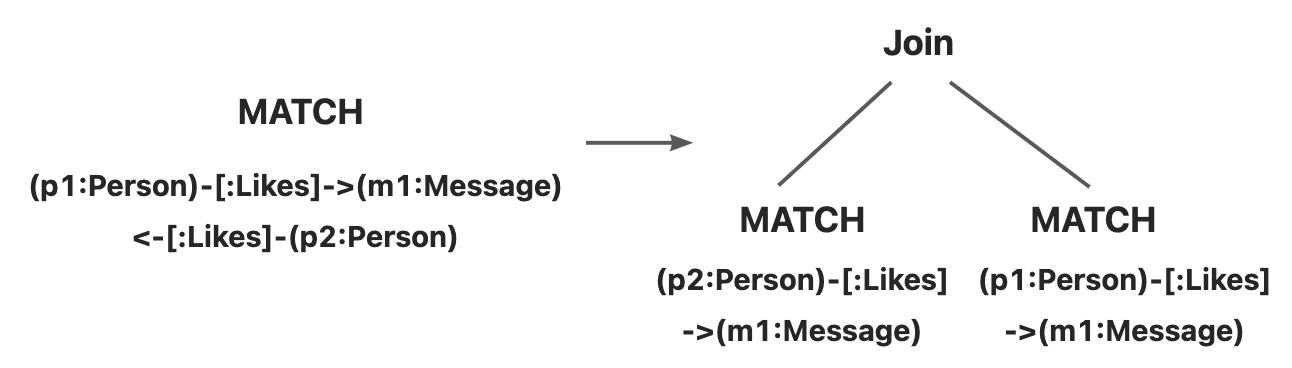
\includegraphics[width=.8\linewidth]{./figures/match-decompose.png}
    \caption{Decomposion of the match operator in the SPJM query shown in Fig.~\ref{fig:spjm}.}
    \label{fig:match-decomposition}
\end{figure}

\begin{example}
    Given the matching operator in Fig.~\ref{fig:spjm}, it is decomposed into two matching operators as shown in Fig.~\ref{fig:match-decomposition}.
    For the right matching operator, because its pattern is a complete star $(p_1, \{m_1\})$, the operator is an MMC.
    For the left matching operator, as its pattern is an edge pattern, it is also an MMC.
    Therefore, the decomposition tree cannot be further decomposed and is a logical plan.
\end{example}

\subsection{Comparision of Search Space}
\label{sec:compare-search-space}

The search space complexity of the decomposition-based method differs greatly from that of the straightforward method for optimization.
In this subsection, we compare the complexities with theoretically analysis.
For simplicity, we focus on the search space of join order optimization and the selection and projection operators are omitted.

Specifically, for the straightforward method, the matching operator is transformed into a sequence of join operators between relations representing vertices and edges.
Therefore, the join order can be optimized with any relational optimizer.
Since Calcite \cite{calcite,columbia} is one of the most widely adopted optimizers for relational databases, it is utilized as a representative of relational optimizers in this analysis.

For the decomposition-based method, given a matching operator $\matching(GR, \pattern)$ in an SPJM query, the outputs of the join operators in the decomposition tree are all induced subgraphs of $\pattern$.
This is consistent with the requirements of GLogS \cite{GLogS}, which is one of the state-of-the-art graph optimizers.
Therefore, the obtained plan is optimized with GLogS.

The complexity of optimization with Calcite is analyzed first.
\begin{theorem}
    \label{theorem:complexity-of-calcite}
    Given $n + m$ relations joined together, $n$ of them representing vertcies and $m$ representing edges, the complexity of join order optimization with Calcite is at least $O(4^{m+n-1})$.
\end{theorem}
\begin{proof}
    We first construct a graph with these $n + m$ relations.
    Specifically, each relation corresponds to a vertex in this graph, and if there is a join condition w.r.t.~two relations, there is an edge between the corresponding vertices.
    To avoid cross product, everytime two relations are joined together, there should be join conditions between them.
    Therefore, the join order can be represented as a spanning tree in the graph.
    By computing the number of physical plans can be generated according to each spanning tree, the total number of physical plans can be obtained.

    In this proof, we compute the number of physical plans for one spanning tree, and this number is a lower bound of the number of physical plans that can be generated.

    We start with a spanning tree with $k$ edges ($k \geq 1$), which has only one leaf node (i.e., it is a path).
    Then, the number of logical plans corresponding to the spanning tree is
    \begin{equation*}
        \begin{split}
            c_l(k) & = 2 * (c(0)c(k-1) + c(1)c(k-2) + \cdots + c(k-1)c(0)) \\
            & = 2\Sigma_{i=0}^{i=k-1}c(i)c(k-1-i), \\
            & \text{where } c_l(0) = 1.
        \end{split}
    \end{equation*}
    With the generating function, it is obtained that
    \begin{equation*}
        \begin{split}
            c_l(k) & = \frac{2^k}{k+1}C(2k, k) \geq \frac{2^k}{k+1}\frac{2k \times \cdots \times (k+1)}{k \times \cdots \times 1} \\
            & \geq \frac{2^k}{k+1}2^{k-1}(k+1) = \frac{4^k}{2}
        \end{split}
    \end{equation*}

    For any spanning tree $T$ with $k = m + n - 1$ edges, denote the longest path in the tree by $p_1$, and its length is $P_1 = |p_1|$.
    By removing the path (i.e., edges in $p_1$) from $T$, we can obtain a new subgraph $T_1$.
    Similarly, the longest path in $T_1$ that intersects with the already removed paths (i.e., $p_1$) is obtained and denoted by $p_2$, with $P_2 = |p_2|$.
    After that, $p_2$ is removed from $T_1$ and subgraph $T_2$ is obtained.
    For $p_1$ and $p_2$, since they are both paths, the numbers of logical plans corresponding to them are $c_l(P_1)$ and $c_l(P_2)$, respectively.
    Without loss of generality, suppose $p_1$ and $p_2$ intersects at vertex $v_i$, and then, $v_i$ appears in each logical plan corresponding to $p_1$.
    Then, by replacing $v_i$ with the plans corresponding to $p_2$, respectively, $c(p_1 \cup p_2) \geq c_l(P_1)c_l(P_2)$ plans are obtained, where $c(t)$ is the number of logical plans corresponding to tree $t$ and $c(t) = c_l(k)$ when $t$ is a path with $k$ edges.

    As $T$ is a tree, by repeatedly finding and removing the paths as above, all the edges in $T$ are finally removed.
    Let the number of paths removed be $s$, we have
    \begin{equation*}
        \begin{split}
            c(T) & = c(p_1 \cup \cdots \cup p_s) \geq c_l(P_1) \cdots c_l(P_s) \\
            & \geq \frac{4^{P_1 + \cdots + P_s}}{2^s} = \frac{4^{m + n - 1}}{2^s} \geq 2^{m+n-1}.
        \end{split}
    \end{equation*}

    %Thus, the number of logical plans w.r.t.~a spanning tree is
    %\begin{equation*}ƒ
    %    \frac{2^{m+n-1}}{m+n}C(2m+2n-2, m+n-1) \geq \frac{4^{m+n-1}}{m+n}.
    %\end{equation*}


    Thus, the number of physical plans is at least $2^{m+n-1}t^{m+n-1} \geq 4^{m+n-1}$, so is the complexity of join order optimization with Calcite.

    In conclusion, Theorem \ref{theorem:complexity-of-calcite} is correct.
\end{proof}

Then, we analyze the complexity of optimization with GLogS.

\begin{theorem}
    \label{theorem:complexity-of-glogue}
    Given a matching operator whose pattern graph consists of $n$ vertices and $m$ edges, the complexity of join order optimization with GLogS is smaller than $3^n$.
\end{theorem}
\begin{proof}
    Since the considered patterns are all induced subgraphs in GLogS, the complexity of join order optimization is not related to the number of edges (i.e., $m$).
    Then, the join order optimization problem is reduced to a variant of the shortest path problem, and the complexity is $O(\mathcal{E})$, where $\mathcal{E}$ is the number of edges in GLogue.
    In detail,
    \begin{equation*}
        \begin{split}
            %O(\mathcal{E}) & = C(n, n-1)*(2^{n-1}-1) + C(n, n-2) * (2^{n-2}- 1) \\
            %& + \cdots + C(n, 1) * (2^1 - 1) \\
            O(\mathcal{E}) & = \Sigma_{i=1}^{i=n-1}C(n, i)(2^i - 1) = 3^n - 2^{n+1} +1 < 3^n.
        \end{split}
    \end{equation*}

    In conclusion, Theorem \ref{theorem:complexity-of-glogue} is correct.

\end{proof}

Based on the complexity analysis in Theorem \ref{theorem:complexity-of-calcite} and Theorem \ref{theorem:complexity-of-glogue}, it is found that when there is only a matching operator,
\begin{equation*}
    \begin{split}
        \frac{\text{Complexity of Calcite}}{\text{Complexity of relgo}} & > O(\frac{4^{m+n-1}}{3^n}) = O(4^{m-1}(\frac{4}{3})^n).
    \end{split}
\end{equation*}
Therefore, it suggests that GLogS is exponentially faster than Calcite in optimizing matching operators.
It also illustrates the superiority of the decomposition-based method.

\iffalse
\section{Solutions for SPJM Problem}
Two techniques can be applied to assist in solving the SPJM problem.
Since the inputs of matching operators include a graph relation that can be represented as a property graph and a pattern, this process can be regarded as querying on graphs.
Then, the graph structure can be leveraged to generate better plans.
Moreover, in a graph, vertices and edges do not have to be joined one by one and the results of specific substructures can be obtained more efficienctly.
In this section, we first introduce the concepts of the above techniques, and then present different types of methods for solving the SPJM problem.

\subsection{Graph Structure}

The definition of graph structure is as follows.

\begin{definition}[Graph Structure, abbr.~GS]
    Graph structure refers to the connectivity relationships between vertices and edges within the graph, which can be stored in graph indices in varied data structure such as adjacent lists.
\end{definition}

With graph structure, tables can be joined more efficiently.
For example, when two tables representing persons and friendships respectively are joined together, the rows that can be joined are quickly located using graph indices.
Therefore, when graph indices are available, using join methods that can leverage graph indices is a more efficient choice.

\subsection{Graph Matching Decomposition}

A matching operator can be decomposed into two new matching operators.
By joining the results of the new matching operators, the results of the original matching operator can be obtained.
Decomposing the matching operator recursively can result in a tree, which is called the match scanning plan.
Each tree node represents an operator.
\textbf{Without loss of generality, the left-deep join order is employed on the tree}.
Each internal node represents an operator including the join, selection, and projection operator.
Please note that these operators in the tree always map graph relations to graph relations, because in the matching process, graph elements are the smallest units that operators can manipulate.

For internal nodes representing join operators, they are generated when matching operators are decomposed.
Suppose a matching operator $TN_0 = \mathcal{M}(GR, \mathcal{P}_0)$ is decomposed into two child operators, i.e., $TN_1 = \mathcal{M}(GR, \mathcal{P}_1)$ and $TN_2 = \mathcal{M}(GR, \mathcal{P}_2)$.
Denote the sets of vertices and edges in a pattern $\mathcal{P}$ by $\mathcal{P}.V$ and $\mathcal{P}.E$, respectively.
Then, we have $\mathcal{P}_0.V = \mathcal{P}_1.V \cup \mathcal{P}_2.V$, $\mathcal{P}_0.E = \mathcal{P}_1.E \cup \mathcal{P}_2.E$, $\mathcal{P}_1.V \cap \mathcal{P}_2.V \neq \emptyset$, and $\mathcal{P}_1.E \cap \mathcal{P}_2.E = \emptyset$.
After $TN_0$ is decomposed, it is transformed to an internal node representing the join operator, with $TN_1$ and $TN_2$ being its child nodes.


Each leaf node of the match scanning plan is a minimum matching component, and the definition is as follows.

\begin{definition}[Minimum Matching Component, abbr.~MMC]
    A matching operator is called a minimum matching component iff the matching of the pattern has a specific physical implementation according to the optimizer and the matching operator will not be further decomposed.
\end{definition}

In the process of decomposing the matching operator, an important point is the order in which the nodes and edges are decomposed each time.
In other words, it is crucial to determine the order of the joins to generate the pattern specified in the original matching operator.
Therefore, optimizers are applied to optimize the match scanning plan.
In this paper, optimizers utilized in relational databases (e.g., Calcite) are called relational optimizers and those applied in graph databases (e.g., GLogS) are called graph optimizers.

For relational optimizers, the MMCs are matching operators whose patterns only contain a vertex or an edge.
Then, the physical implementation of such matching operators is scanning the tables of the corresponding vertices or edges, respectively.
Therefore, for relational optimizers, the matching operator will be replaced with selection operators, projection operators, and a sequence of join operators between tables representing vertices and edges.

For graph optimizers, the MMCs are more diverse.
Following the idea of StarJoin \cite{starjoin,huge}, matching operators whose patterns consist of a vertex, an edge, or a complete star are considered as MMCs.
Here, the pattern consisting of an edge actually contains the edge and its adjacent two vertices.
A complete star is a special structure on a graph.
Let $TL = \mathcal{M}(GR, \mathcal{P})$ be an MMC, which is also a leaf node of the tree, and $\mathcal{P}$ is a complete star.
Also, denote the parent node of $TL$ by $Join_{TL}$.
A complete star is a tree of depth one with at least three vertices, whose root is called the core, while the other nodes are called the outsiders.
For each outsider $v_o$ of a complete star, $v_o$ should exist in the pattern of matching operators in $Join_{TL}$'s left subtree.
Besides, $TL$ should be the right subtree of $Join_{TL}$.
Otherwise, $TL$ is not a minimum matching componet and should be further decomposed.

For the MMC whose pattern is a vertex, it is implemented with scanning the corresponding table.

For the MMC whose pattern is an edge, if graph strucutre is utilized, it can be implemented with joins that leverage graph indices, and the neighbors of vertices can be obtained efficiently.
If graph structure is not utilized, such a pattern is obtained by two joins between tables representing vertices and edges.


For the MMC whose pattern is a complete star, it can be implemented with a table scan of the core.
The outsiders are not handled, because they are already computed in the left subtree of the parent node of MMC.
MMC's parent node representing the join operator is then implemented with extend-intersection.
Specifically, in the process of extend-intersection, the neighbors of the outsiders are obtained by joining them with tables representing edges and the results of MMC, respectively.
The common neighbors are obtained by calculating the intersection.
Please note that if graph structure is available, the neighbors can be obtained with graph indices.
With extend-intersection, the times of joins are reduced significantly, and it has better performances than joining tables one by one.


Moreover, for optimizers, cost of different join orders should be evaluated.
Normally, the cost is estimated with the numbers of vertices and edges with different labels, which are obtained by counting the rows of the corresponding tables.
These are low-order statistics in graphs.
Since matching operators perform pattern matching on graphs, it is more efficient to estimate the cost with graph statistics.

\begin{definition}[Graph Statistics]
    Graph statistics record the occurrence of structures within the graph, such as the number of triangles appearing in the graph.
\end{definition}

Specifically, graph statistics can reflect the higher-order features of graphs (e.g., the number of subgraphs), and well represent the characteristics of graphs.
Thus, with garph statistics, better join orders with lower cost can be obtained.

The aforementioned optimizations are collectively referred to as optimizations based on graph matching decompostion (abbr.~GMD).


\subsection{Different Types of Methods}
\label{sec:different-type-of-methods}

The general approach to handling the SPJM queries is to first transform it into an SPJ queries, and then optimize the SPJ queries to obtain the corresponding physical plans.
It is proved in Theorem \ref{theorem:spjm-to-spj} that SPJM queries can always be losslessly converted to SPJ queries.
Existing methods can be divided into four categories based on whether GS and GMD are utilized in the process.

(1) \emph{\textbf{Translator}: SPJM $\rightarrow$ SPJ $\rightarrow$ Physical Plan}.

Translators do not apply GS and GMD in the process of optimizing the SPJM queries.
In detail, matching operators are decomposed into minimum matching components, whose patterns contain only a vertex or an edge.
Such matching operators are converted to table scans, and a new SPJ query is generated and optimized.
This type of method degrades into relational optimizers and loses the chance of query optimization from the graph perspective.
Typical methods of this type include Apache Age \cite{apache-age} and DuckPGQ \cite{DuckPGQ,DuckPGQ-VLDB}.


In order to leverage the graph information to obtain better physical plans, the second kind of method is proposed.

(2) \emph{\textbf{Post-processor}: SPJM $\rightarrow$ SPJ $\xrightarrow{GS}$ Physical Plan}.

For this type of method, graph structure is utilized in the process of optimizing the SPJ queries.
Specifically, with graph indices, the connectivity between vertices and edges can be obtained efficiently.
Therefore, new physical implementations of joins can be constructed to leverage the benefits of graph indices.

The optimizer in GrainDB is a representative of this type.
GrainDB builds RID indices on DuckDB \cite{duckdb}, and proposes two new join methods, i.e., sip-join and merge-sip-join.
In detail, sip-join gets adjacent edges of vertices or gets adjacent vertices of edges based on the RID indices, while merge-sip-join obtains the neighbors of vertices.
Given a SPJM query, it is first transformed to the equal SPJ query, and then GrainDB optimizes the query with the relational optimizer of DuckDB to obtain the optimal execution plan.
Next, GrainDB replaces some hash-joins in the plan with sip-joins and merge-sip-joins to leverage graph indices.

It indicates that the cost-based optimization in GrainDB only finds the optimal execution plan before the graph indices are awared.
Therefore, the plan can be suboptimal after replacement.
Moreover, some efficient replacement cannot be applied w.r.t.~the obtained execution plan due to the order of joining tables representing vertices and edges.


It is also reasonable to exploit the capability of graph matching decomposition for better optimization.
Then, the third kind of method is proposed as follows.

(3) \emph{\textbf{Sorter}: SPJM $\xrightarrow{GMD}$ SPJ $\rightarrow$ Physical Plan}.

This type of method converts SPJM queries to SPJ queries in a different manner.
Specifically, graph matching decomposition is applied and the matching of complete stars is a minimum matching component.
With GMD, higher-order features of graphs are leveraged, and cost of join orders can be estimated more accurately.
Please note graph structure is not applied in this type of method.
Thus, when we optimize SPJ queries and generate physical plans, the physical implementations of joins cannot utilize the graph indices, including the implementation of extend-intersection.


(4) \emph{\textbf{Optimizer}: SPJM $\xrightarrow{GMD}$ SPJ $\xrightarrow{GS}$ Physical Plan}.

This is the method utilized in this paper.
Compared to method (3), this kind of methods further utilize graph strucutre in optimization.
Therefore, physical implementations of join operators can utilize the graph indices and the common neighbors can be obtained more efficiently in extend-intersection.
Besides, in the process of graph matching decomposition, since the higher-order statistics are utilized (i.e., the number of subgraphs), the cost of joins are estimated assuming that graph indices can be utilized in execution.
Therefore, cost estimation is more accurate for when graph indices are applicable.

\subsection{Feasibility of Converting SPJM Queries to SPJ Queries}
In this subsection, we prove that SPJM queries can always be converted to SPJ queries.
Therefore, it is possible to leverage relational databases to process matching operators, and the methods proposed in Sec.~\ref{sec:different-type-of-methods} are workable.

\begin{theorem}
    \label{theorem:spjm-to-spj}
    The SPJM query can be losslessly converted to an SPJ query.
\end{theorem}
\begin{proof}
    Clearly, if the matching operator can be expressed with selection, projection, and join operators (abbr.~SPJ operators), then naturally, the theorem is correct.
    We first discuss the matching operators under the semantics of homomorphism and prove the theorem by induction.
    % We begin with matching operators with homomorphic semantics, and prove the theorem using induction.
    In this proof, vertices and edges are elements in a pattern and a pattern $\mathcal{P}$ is called a strict pattern, if the adjacent vertices of each edge in $\mathcal{P}$ are specified in the pattern (e.g., (u)-[e]-(v)).
    Otherwise, the pattern is called a loose pattern (e.g., (u)-[e]).
    Without the loss of generality, matching operator $\mathcal{M}(GR, \mathcal{P})$ is considered.
    Then, induction is conducted on the number of elements in $\mathcal{P}$.

    When there is only one element in $\mathcal{P}$ (e.g., $\mathcal{P}=(u:\text{Person})$), such a pattern can be expressed with the selection operators (e.g., $\sigma_{label=\text{``Person''}}(V)$).
    Please note that if there are more constraints on the element (e.g., the returned person should be at least 18 years old), more constraints can be specified with the selection operators.

    Suppose for patterns with at most $n$ elements, they can be expressed with SPJ operators.
    Denote the sequence of SPJ operators that have the same meaning as pattern $\mathcal{P}$ by $\mathcal{E}_{\mathcal{P}}$.
    When there are $n+1$ elements in a pattern $\mathcal{P}$, let $v$ be a vertex in $\mathcal{P}$, and $e_1, \cdots, e_k$ are the edges adjacent to $v$. %connecting $v$ with the other vertices in $\mathcal{P}$.
    $\widehat{\mathcal{P}}$ is the strict pattern obtained by removing $v$ and $e_1, \cdots, e_k$ from $\mathcal{P}$.
    Then, $\mathcal{P}$ can be expressed with SPJ operators as follows:
    \begin{equation*}
        \mathcal{E}_{\widehat{\mathcal{P}}} \Join \sigma_{label=el_1}(E) \Join \cdots \Join \sigma_{label=el_k}(E) \Join \sigma_{label=vl}(V),
    \end{equation*}
    where $vl$ is the label of $v$, $el_1, \cdots, el_k$ are labels of $e_1, \cdots, e_k$.
    In conclusion, adopting the homomorphism semantics, the matching operator can be expressed with SPJ operators.

    Furthermore, when the matching operator adopt other semantics (e.g., isomorphism), it is straightforward to add some constraints on the elements with selection operators.
    For instance, when the isomorphism semantics is adopted, constraints should be added to ensure that different vertices in the pattern graph match with different vertices in the database.
    Therefore, the theorem is correct.
\end{proof}
\fi

%\section{Physical Implementation of Logical Operators}

Given an SPJM query, the selection, projection, and join operators are performed on relations and have the same physical implementations as those in relational databases.
The main difference lies in the physical implementation of matching operators.
In detail, if the graph-agnostic method in \refsec{solve-spjm-problem} is applied, the obtained logical matchings plans consist of selection, projection, and join operators.
Otherwise, if the graph-aware method is applied, the logical matching plans additionally include matching operators.
In this section, we focus on the physical implementions of the operators in logical matching plans.
Specifically, we focus on the join operators and matching operators in logical matching plans, because there can be many variations in the physical implementation of these two operators and the query performance varies greatly among different implementations. 
In this section, we first propose the concept of graph indices and then present the physical implementations of join and matching operators.

\begin{figure}
    \centering
    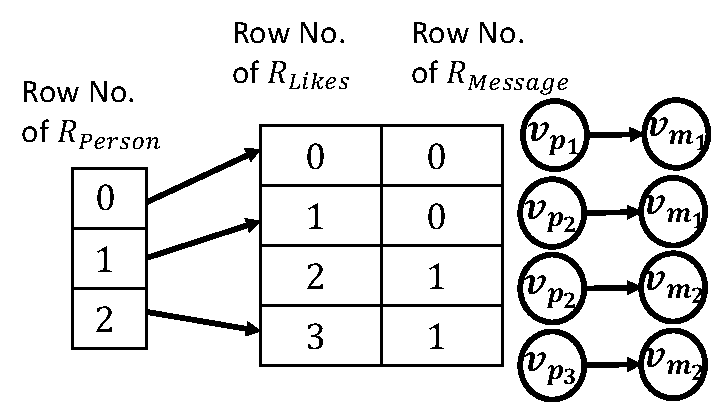
\includegraphics[width=.8\linewidth]{./figures/graph-index-likes.pdf}
    \caption{A graph index on edges labeled ``Likes'' on $G_1$ in \reffig{intro-rgmapping-example}.}
    \label{fig:graph-index}
\end{figure}

\subsection{Graph Index}
\label{sec:graph-index}

In a property graph, the adjacency relationships between vertices and edges are obvious and the adjacent edges of a vertex can be obtained directly.
Moreover, a tuple in a relation corresponds to a vertex or an edge in the property graph according to the \rgmapping.
Therefore, by maintaining the relationships between vertices and edges via indices, the join operator can be markedly accelerated. 
This improvement is achieved because for each tuple within a relation, the indices have pre-stored the tuples that are joinable with it. 
As a result, it eliminates the necessity to iterate through every tuple of the counterpart relation, thereby enhancing the efficiency of the join process.
As this index structure mimics the adjacency relationship between vertices and edges, it is called a graph index.

Join operators that leverage graph indices are called predefined joins by GrainDB \cite{graindb}.
Specifically, an example of the graph index instantiated in GrainDB is shown in \reffig{graph-index}.
In detail, the graph index is built on edges labeled ``Likes'' in property graph $G_1$ of \reffig{intro-rgmapping-example}(a) and records the adjacency relationships of the vertices labeled ``Person'' and the edges labeled ``Likes''.
That is, according to the \rgmapping, for each tuple $t_p$ in $\relation{Person}$, the tuples in $\relation{Likes}$ that can be joined with $t_p$ can be directly obtained with the graph index and vice versa.

In detail, the graph index consists of two parts as shown in \reffig{graph-index}.
The first part in \reffig{graph-index}(a) is designed for efficiently accessing tuples in $\relation{Person}$ that can be joined with tuples in $\relation{Likes}$.
Specifically, a new column named ``pid\_rowid'' is added to $\relation{Person}$ and the new relation with more columns is called $\grelation{Person}$.
For each tuple $t \in \grelation{Person}$, $t.pid\_rowid$ is the row number of $t_p \in \relation{Person}$, where $t_p.person\_id = t.pid$.
Note that row numbers start from 0.
Take the first tuple in $\grelation{Likes}$ (denoted as $t_l$) as an example.
Because $t_l.pid = p_1$ and the tuple $t_p$ at row number 0 in $\relation{Person}$ satisfies $t_p.person\_id = p_1 = t_l.pid$, we have $t_l.pid\_rowid = 0$.
With this graph index, given a tuple $t$ in $\grelation{Likes}$, the tuple in $\relation{Person}$ that are joinable with $t$ can be retrieved without scanning $\relation{Person}$.

However, given a tuple $t_p$ in $\relation{Person}$, we cannot leverage the graph index in \reffig{graph-index}(a) to directly access tuples in $\grelation{Likes}$ joinable with $t_p$, because it is unknown which rows of $\grelation{Likes}$ contain $pid$ values equal to $t_p.person\_id$.
Therefore, the adjacency list in \reffig{graph-index}(b) is constructed to solve this problem.
To elaborate, the first column contains the row numbers in $\relation{Person}$.
For example, row number 1 represents the second tuple in $\relation{Person}$ with $person\_id = p_2$ (denoted by $t_{p_2}$) and this tuple corresponds to $v_{p_2}$ in $G_1$.
The second column records the row numbers in $\grelation{Likes}$.
With this column, the edges adjacent to a given vertex can be retrieved efficiently.
For example, the edges adjacent to $v_{p_2}$ (i.e., $e_{l_2}$ and $e_{l_3}$ in $G_1$) are stored at row 1 and row 2 of $\grelation{Likes}$.
It means that the second and third tuples in $\grelation{Likes}$ can be joined with $t_{p_2}$.

If the adjacent relationships between vertices labeled ``Message'' and edges labeled ``Likes'' are also recorded in this index, the third column in \reffig{graph-index} is added.
With this column, the neighbors of given vertices can be quickly accessed.
It means that given a tuple $t_p$ in $\relation{Person}$, let $T_{Likes}$ be the set of tuples in $\relation{Likes}$ which can be joined with $t_p$, and then the tuples in $\relation{Message}$ which can be joined with a tuple in $\relation{Likes}$ can be quickly obtained.
For example, the neighbors connected to $v_{p_2}$, connected through edges labeled ``Likes'', include $v_{m_1}$ and $v_{m_2}$, whose corresponding tuples are at row 0 and row 1 in $\relation{Message}$.
This information can be quickly ascertained through the graph index.

\subsection{Physical Implementation of Join and Matching Operators}
\label{sec:join-matching-operator}
In a logical matching plans, the inputs of join operators are two graph relations, i.e., $GR_1 \widehat{\Join} GR_2$.
The join operators can be divided into three categories based on $GR_2$.

Firstly, if $GR_2$ is not obtained by a matching operator, then the join operator is implemented with 
\begin{equation*}
    \widehat{\pi}_{A_1}(GR_1) \Join \widehat{\pi}_{A_2}(GR_2),
\end{equation*}
where $A_1$ and $A_2$ are lists of all the attributes of vertices and edges in $GR_1$ and $G_2$, respectively.

Secondly, if $GR_2$ is obtained by a matching operator whose pattern graph is an edge, then the join operator is implemented as an \expandvertex~operator. 
Specifically, denote the matching operator by $\matching(\pattern_e)$, where $\pattern_e$ consists of two vertices $u_s, u_t$ and an edge $e$ connecting them.
Let $\lambda_s$ and $\lambda_t$ be functions that associate tuples in $\relation{\vlabel{(e)}}$ with those in $\relation{\vlabel(u_s)}$ and $\relation{\vlabel(u_t)}$, respectively.
Then, the \expandvertex~operator is implemented with 
\begin{equation*}
    \widehat{\pi}_{A_1}(GR_1) \Join \relation{\vlabel{(u_s)}} \Join \relation{\vlabel{(e)}} \Join \relation{\vlabel{(u_t)}}.
\end{equation*}
If graph indices have been built on $\relation{\mathcal{L}(e)}$, the joins between $\relation{\mathcal{L}(u_s)}$, $\relation{\mathcal{L}(e)}$, and $\relation{\mathcal{L}(u_t)}$ can be implemented more efficiently by leveraging the graph indices.
Moreover, if there is no need to retain attributes on $e$ and there are no constraints on $e$, graph indices can be applied to get neighbors of $u_s$ directly without scanning $\relation{\mathcal{L}(e)}$.

Thirdly, if $GR_2$ is obtained by a matching operator whose pattern graph is a complete star, then the join operator is implemented as an \expandintersect~operator.
Denote the matching operator by $\matching(\pattern_s)$, where $\pattern_s = (v_r; \mathcal{H})$ and $\mathcal{H} = \{v_1, \cdots, v_k\}, k \geq 2$.
Let $e_1, \cdots, e_k$ be the edges connecting $v_1, \cdots, v_k$ and $v_r$, respectively.
Moreover, let $\lambda^{e_i}_s$



\subsection{Join Operators}
\label{sec:join-operator}
There are two kinds of join operators, where $\Join$ is defined over relations while $\widehat{\Join}$ is defined over graph relations.

For the first type of join operator (i.e., $\Join$), it is always utilized to ensure the adjacency relationships between vertices and edges.
For example, the join operator in $\relation{Person} \Join \relation{Likes}$ is used to ensure that the obtained edges labeled ``Likes'' are adjacent to vertices labeled ``Person''.




For the second type of join operator (i.e., $\widehat{\Join}$), if its right subtree is an matching operator $\matching(\pattern)$ whose pattern graph is a complete star, this join operator is denoted by $\widehat{\Join}_{ei}$ and implemented with extend-intersection.
Specifically, let \(\pattern = (v_r; \mathcal{H})\), $\mathcal{H} = \{v_1, \cdots, v_k\}, k \geq 2$, and denote the inputs of the join operator by $\relation{1}$ and $\relation{2}$, respective.
Then, an intuitive method to implement the join operator is as follows:
\begin{equation*}
    R_{1} \Join R_{\mathcal{L}(e_1)} \Join \cdots \Join R_{\mathcal{L}(e_k)} \Join R_{2},
\end{equation*}
where $e_x = (v_x, v_r), k \geq x \geq 1$.
However, in this process, the results must be instantiated once after each join is completed and numerous intermediate results are instantiated, significantly reducing query performance.

Please note that different edges (i.e., $e_1, \cdots, e_k$) intersect at the same vertex $v_r$.
Therefore, the intersection can be applied before the results are instantiated and fewer intermediate results are generated.
Then, the efficiency can be noticeably enhanced.

Moreover, if graph indices on $e_1, \cdots, e_k$ are available, the efficiency of the joins can be further improved by leveraging the graph indices to access joinable tuples quickly.


\subsection{Matching Operators}
\label{sec:matching-operator}
According to the graph-aware method, the matching operators in logical matching plans are all MMCs.
Specifically, based on different pattern graphs, MMCs in logical matching plans can be divided into two categories: 
(1) Matching Operators whose pattern graph is a complete star, denoted by $\matching_{star}$;
(2) Matching Operators whose pattern graph is an edge, denoted by $\matching_{edge}$.

For $\matching_{star}$, suppose its pattern graph is $\pattern = (v_r; \mathcal{H})$, it is implemented by scanning $\relation{\mathcal{L}(v_r)}$.

For $\matching_{edge}$, suppose the pattern is $(u_s) - [e] \rightarrow (u_t)$, then the matching operator is implemented by $\relation{\mathcal{L}(u_s)} \Join \relation{\mathcal{L}(e)} \Join \relation{\mathcal{L}(u_t)}$.
According to \refsec{join-operator}, if graph indices have been built on $\relation{\mathcal{L}(e)}$, these two joins can be implemented more efficiently by leveraging the graph indices.
Moreover, if there is no need to retain attributes on $e$ and there are no constraints on $e$, graph indices can be applied to get neighbors of $u_s$ directly without scanning $\relation{\mathcal{L}(e)}$.


\section{Optimizing Matching Operator}
\label{sec:optimizing-matching-operator}
In this section, we focus on handling the matching operator (more precisely, the graph component),
which plays a distinct role within the \spjm queries compared to the \spj queries. We discuss two main perspectives of optimizing
the matching operator: logical transformation and physical implementation. Logical transformation is
responsible for transforming a matching operator into a logically equivalent representation,
while physical implementation focuses on how the matching operator can be efficiently executed.


%\enlargethispage{1em}
\subsection{Logical Transformation}
\label{sec:handling-match-operator}
We commence with an intuitive, graph-agnostic transformation before
introducing a graph-aware technique grounded on the concept of decomposition tree, which
is the key to the optimization of graph pattern matching in the literature~\cite{huge,GLogS}.

Before proceeding, we introduce the concept of pattern decomposition that decomposes $\pattern$ into two overlapping patterns, $\pattern_1$ and $\pattern_2$, with shared vertices $V_{o} = V_{\pattern_1} \cap V_{\pattern_2}$ and shared edges $E_{o} = E_{\pattern_1} \cap E_{\pattern_2}$.
Denote $\pattern = \pattern_1 \cup \pattern_2$. Under the homomorphism semantics, the matching of $\pattern$ can be represented as:
\begin{equation}
    \label{eq:join-pattern}
    \matching(\pattern) = \matching(\pattern_1) \widehat{\Join}_{V_{o}, E_{o}} \matching(\pattern_2),
\end{equation}
where $\widehat{\Join}$ is a natural join operator for joining two graph relations based on the common vertices and edges.

It is important to note that \refeq{join-pattern} is also applicable to alternative semantics, including isomorphism and non-repeated-edge~\cite{angles2017foundations}. To support these semantics, a special all-distinct operator can be applied as a filter to remove results that contain duplicate vertices and/or edges. The adoption of the all-distinct operator is compatible with all techniques in this paper.

%There are already a considerable number of research findings and solutions for the SPJ problem \cite{}.
%Given that the main difference between SPJM and SPJ lies in the matching operator, in addressing the SPJM problem, solutions from the SPJ problem can be referenced.
%In this section, we focus on the method to deal with the matching operators.
%Firstly, an intuitive method is presented and then an advanced method based on matching decomposition is proposed.
%For simplicity, the pattern graph given in matching operators are assumed to be connected in this section.

%\enlargethispage{1em}

\subsubsection{Graph-agnostic Transformation}
\label{sec:intuitive-method}
If the matching operator can be transformed into purely relational operations, the \spjm query becomes a
standard \spj query, which can then be optimized using existing relational optimizers (\refsec{relational-only}). This graph-agnostic
approach is intuitive and easy to implement on top of existing relational databases, making it a straightforward
choice in prototyped systems~\cite{apache-age,DuckPGQ,DuckPGQ-VLDB}. However, there is no theoretical guarantee that
such a transformation is lossless in the context of \rgmapping. In this subsection,
we bridge this gap by demonstrating the lossless transformation of the matching
operator under \rgmapping.
% aim to
%Graph-agnostic methods~\cite{apache-age,DuckPGQ,DuckPGQ-VLDB} simply recast graph match operations
%as a sequence of relational operations (mainly joins and projections). This allows an \spjm query to be naively transformed into an \spj query, which then can be optimized through standard relational optimizers.

Consider a pattern graph $\pattern$ and one of its edges $e = (u_s, u_t)$. According to the definition of the matching operator (\refsec{matching-operator}), the graph edges and vertices that can be matched with $e$ must have the labels $\lab(e)$, $\lab(u_s)$, and $\lab(u_t)$. We further denote the relations corresponding to these edges and vertices via \rgmapping as $R_{\lab(e)}$, $R_{\lab(u_s)}$, and $R_{\lab(u_t)}$, respectively. Moreover, there must be total functions $\lambda_{\lab(e)}^s$ and $\lambda_{\lab(e)}^t$ for mapping tuples from $R_{\lab(e)}$ to $R_{\lab(u_s)}$ and $R_{\lab(u_t)}$, respectively. We define the following \EVjoin relational operation regarding $\lambda_{\lab(e)}^s$ as:
\begin{equation} \label{eq:ev-join}
\begin{split}
R_{\lab(e)} & \evjoin R_{\lab(u_s)} = \{(\tau_e, \tau_s) \;|\; \\
  &  \tau_e \in R_{\lab(e)} \land \tau_s \in R_{\lab(u_s)} \land \lambda_{\lab(e)}^s(\tau_e) = \tau_s\}.
\end{split}
\end{equation}
The \EVjoin regarding $\lambda_{\lab(e)}^t$ is defined analogously. Although called \EVjoin, the operation is associative like any relation join, meaning that the order in which the edge and vertex relations are joined does not affect the final result.


%Such a transformation, as indicated by the following lemma, maintains the integrity of the data and relationships, ensuring a lossless conversion process.
%The following lemma demonstrates that, in an \spjm query, the matching operation can be losslessly transformed into a sequence of purely relational operations.
We have the following lemma.%\footnote{Omitted proofs can be found in the supplementary material.}.


\begin{lemma}
    \label{lem:spjm-to-spj}
    Under \rgmapping, the matching operation in an \spjm query can be losslessly transformed into a sequence of relational joins involving $n$ vertex relations and $m$ edge relations.
\end{lemma}
\begin{proof}
    Consider a pattern $\pattern_m$ of $m$ edges, where the $i$-th vertex is denoted as $u_i$, and the $i$-th edge is $e_i = (u_{s_i}, u_{t_i})$. %According to the $\rgmapping$, the corresponding relations of vertex $u_i$ and edge $e_i$ are denoted as $\relation{u_i}$ and $\relation{e_i}$, respectively. Furthermore, we have $\lambda_{e_i}^s$ and $\lambda_{e_i}^t$ to map tuples from $\relation{e_i}$ to $\relation{u_{s_i}}$, and from $\relation{e_i}$ to $\relation{u_{t_i}}$, respectively.

The proof proceeds by induction, starting with a pattern graph $\pattern_0$ with a single vertex and no edges. It is clear that $\matching(\pattern_0)$ yields a subset of vertices with label $\lab(u_0)$, which is mapped from the relation $\relation{\lab(u_0)}$ via $\rgmapping$. As a result, we have $R_0 = \gproject(\matching(\pattern_0)) = \relation{\lab(u_0)}$.

Next, consider $\pattern_1$ with one edge, $e_1 = (u_{s_1}, u_{t_1})$. Matching $\pattern_1$ is equivalent to retrieving the edge relation, together with the corresponding source and target vertices. Therefore, we have:
\[ R_1 = \gproject(M(\pattern_1)) = \relation{\lab(u_{s_1})} \evjoin \relation{\lab(e_1)} \evjoin \relation{\lab(u_{t_1})} \]

Assume that when $m = k-1$, $\gproject(\matching(\pattern_{k-1}))$ can be losslessly converted to a sequence of relational operators, resulting in the relation $R_{k-1}$. When $m = k$, we consider $\pattern_{k}$ of $k$ edges that is constructed from $\pattern_{k-1}$ by adding one more edge $e_k = (u_{s_k}, u_{t_k})$. For $\pattern_{k}$ to be connected, it must share at least one common vertex $V_o$ with $\pattern_{k-1}$. According to \refeq{join-pattern}, we have:
\[ \matching(\pattern_{k}) =  \matching(\pattern_{e_k}) \gjoin_{V_o} \matching(\pattern_{k-1}), \]
where $\pattern_{e_k}$ denotes a pattern that contains only the edge $e_k$, and $V_o$ is the common vertex shared by $\pattern_{k-1}$ and $\pattern_{e_k}$. Applying $\gproject$ to the above equation, we get:
\begin{equation*}
\begin{split}
R_k &= \gproject(\matching(\pattern_{k})) \\
    &= \widehat{\pi}_{A_1*}(\matching(\pattern_{e_k})) \Join_{V_o.attr}  \widehat{\pi}_{A_2*}(\matching(\pattern_{k-1})) \\
    &= \relation{\lab(u_{s_k})} \evjoin \relation{\lab(e_k)} \evjoin \relation{\lab(u_{t_k})} \Join_{V_o.attr} R_{k-1}
\end{split}
\end{equation*}
By induction, denoting $R'_i = \relation{\lab(u_{s_i})} \evjoin \relation{\lab(e_i)} \evjoin \relation{\lab(u_{t_i})}$, we have the matching operator losslessly converted to a sequence of relational join operations:
\begin{equation}
    \label{eq:graph-agnostic}
    \gproject(\matching(\pattern_{k})) = R'_k \Join R'_{k-1} \Join \cdots \Join R'_1 \Join R_0.
\end{equation}

We thus conclude the proof.
\end{proof}



%Given that edges may connect to common vertices, it's obvious that there are some redundant joins in \refeq{graph-agnostic}. Removing these redundancies results in
%a sequence of joins involving $n$ vertex tables and $m$ edge tables, as illustrated in the following example.

\begin{example}
  \label{ex:spjm-to-spj}
  Given pattern graph $\pattern$ shown in \reffig{intro-rgmapping-example}(b), the matching operation $\matching(\pattern)$ can be converted to a sequence of join operations as follows. Without loss of generality, we start from $\pattern_0$ containing only the vertex $u_{p_1}$, and we have $\relation{0} = \relationx{1}{\text{Person}}$ (note that the superscript 1 is used to differentiate relations of the same name).
  Next, we sequentially add the edges $e_1 = (u_{p_1}, u_{p_2})$, $e_2 = (u_{p_1}, u_{m})$, and $e_3 = (u_{p_2}, u_m)$ to $\pattern_0$, resulting in the following relations:
  \begin{equation*}
    \begin{split}
    R'_1 &= \relationx{1}{\text{Person}} \Join_{\text{person\_id}=\text{pid1}} \relation{\text{Knows}} \Join_{\text{pid2}=\text{person\_id}} \relationx{2}{\text{Person}}, \\
    R'_2 &= \relationx{1}{\text{Person}} \Join_{\text{person\_id}=\text{pid}} \relationx{1}{\text{Likes}} \Join_{\text{mid}=\text{message\_id}} \relation{\text{Message}}, \\
    R'_3 &= \relationx{2}{\text{Person}} \Join_{\text{person\_id}=\text{pid}} \relationx{2}{\text{Likes}} \Join_{\text{mid}=\text{message\_id}} \relation{\text{Message}}.
    \end{split}
    \end{equation*}

    Finally, we have $\gproject(\matching(\pattern)) = R'_3 \Join R'_2 \Join R'_1 \Join \relation{0}$.
    Note that $\relationx{1}{\text{Person}}$ in $R'_2$, as well as $\relationx{2}{\text{Person}}$ and $\relation{\text{Message}}$ in $R'_3$, are redundant and can be safely removed from the final join. By eliminating these redundant relations, we obtain a sequence of joins involving 3 vertex relations and 3 edge relations.
\end{example}

%\enlargethispage{1em}

\subsubsection{Graph-aware Transformation}
\label{sec:graph-aware}
%The graph-agnostic transformation may be inefficient because relational optimizers treat relations representing vertices and edges equally as the other relations,
%preventing the optimizer from utilizing graph-specific optimization techniques. %Furthermore, relational optimizers are known to struggle with queries containing a large number of joins, which is a common case in graph pattern matching.

We introduce a graph-aware transformation that incorporates key ideas from the literature on graph optimization. Following \refeq{join-pattern}, we can recursively decompose $\pattern$, forming a tree structure called the \emph{decomposition tree}. The tree has a root node that represents $\pattern$, and each non-leaf \emph{intermediate} node is a sub-pattern (a subgraph of the pattern) $\pattern' \subset \pattern$, which has a left and right child node, denoted as $\pattern'_l$ and $\pattern'_r$, respectively. %The condition of the intermediate pattern being induced
The leaf nodes of the tree are called \emph{Minimum Matching Components} (\mmc), correspond to indivisible patterns directly solvable with specific physical operations
as will be introduced in~\refsec{physical-operators}. The decomposition tree naturally forms a logical plan for solving $\matching(\pattern)$, as demonstrated in \reffig{match-decomposition}. For any non-leaf node $\pattern'$, there exists a relationship $\matching(\pattern') = \matching(\pattern'_l) \gjoin \matching(\pattern'_r)$ according to \refeq{join-pattern}. The plan allows for the recursive computation of the entire pattern.

Following state-of-the-art graph optimizers~\cite{huge,GLogS}, to guarantee a \emph{worst-case optimal} execution plan~\cite{ngo2018worst}, all intermediate sub-patterns in the decomposition tree must be induced subgraphs of $\pattern$. Furthermore, \mmc is restricted to be a single-vertex pattern and a \emph{complete star}. A star-shaped pattern is denoted as $\pattern(u;V_s)$, where $u$ is the root vertex and $V_s$ is the set of leaf vertices\footnote{Edge directions between $u$ and $V_s$ are not important, and we assume they all point from $u$ to $V_s$.}. In the decomposition tree, given $\pattern' = \pattern'' \cup \pattern(u;V_s)$, $\pattern(u;V_s)$ is a complete star if and only if it is a right child and $V_s \subseteq V_{\pattern'}$, meaning that the leaf vertices of the complete star must all be common vertices for the decomposition. A single-edge pattern is a special case of a complete star. The complete star logically represents the physical operations of \expandintersect, which will be discussed in \refsec{physical-operators}. As shown in \reffig{match-decomposition}, a single-edge pattern, such as $\pattern_3$, is further decomposed into a single-vertex pattern and the pattern itself, allowing the optimizer to select from which vertex the edge can be expanded.
\revise{The intermediate sub-patterns pruned from the decomposition tree are also presented in \reffig{match-decomposition}}.
\revise{Some previous studies, such as EmptyHeaded \cite{Aberger2016Sigmod} and CLFTJ \cite{Kalinsky2017EDBT}, also generate decomposition trees. However, our method differs significantly from theirs. Specifically, these previous methods operate on hypergraphs, where the vertices correspond to attributes and the edges correspond to relations. In contrast, our decomposition tree is for property graphs, where both vertices and edges correspond to relations. Additionally, in those methods, the leaf nodes do not necessarily have to be a \mmc}.


%The complete star is a logical representation of the physical operations of \expand~and \intersect, which are key to the implementation worst-case optimal join algorithm~\cite{mhedhbi2019optimizing} for graph pattern matching, as will be discussed in \refsec{xx}.

\comment{
Therefore, decomposing the matching operators recursively can finally result in a tree, whose leaf nodes are MMCs.
To ensure worst-case optimality, in the process of decomposition, the pattern graph of each decomposed matching operator should be an induced subgraph of $\mathcal{P}_0$.
The generated tree is called a decomposition tree and it is actually a logical plan of the matching operator.
\modify{Without loss of generality, the left-deep join order is employed on the tree.}

Then, it is crucial to identify which matching operators to treat as MMCs.
We adopt the definition of \emph{complete star} from \cite{huge}.
Specifically, suppose $\matching(GR, \mathcal{P})$ is decomposed into $\matching(GR, \mathcal{P}_1)$ $\widehat{\Join}$ $\matching(GR, \mathcal{P}_2)$, $\mathcal{P}_2$ is called a complete star iff $\mathcal{P}_2$ is a star $(v_r; \mathcal{H})$, $\mathcal{H} \subseteq E_{\mathcal{P}_1}$, and $|\mathcal{H}| \geq 2$, where $v_r$ is the root and $\mathcal{H}$ is the set of its leaf vertices.
Inspired by HUGE \cite{huge} and GLogS \cite{GLogS}, matching operators located on the right subtree of the join operator with complete stars as the pattern graphs are the MMCs in this paper.

Besides, a matching operator located on the left subtree of the join operator is an MMC iff its pattern graph is an edge (i.e., one edge and its adjacent two vertices).
}

\begin{figure}
    \centering
    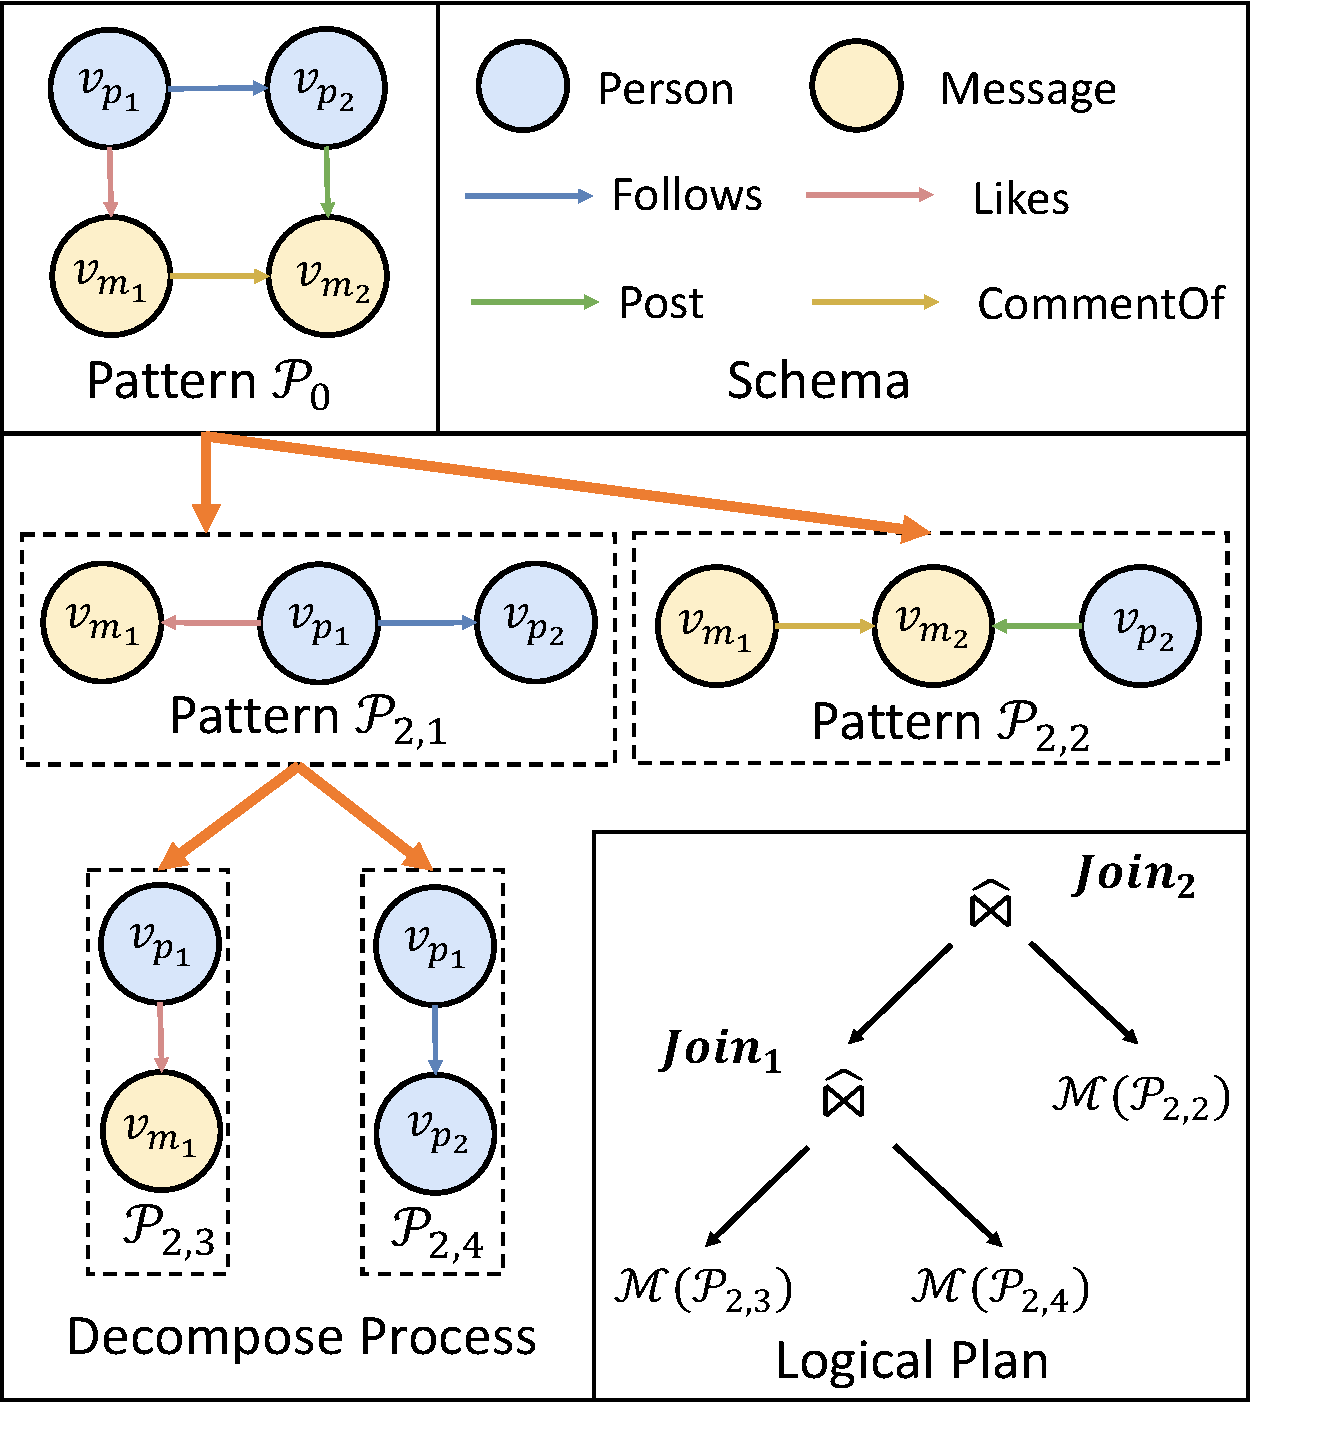
\includegraphics[width=\linewidth]{./figures/decomposition-example.pdf}
    \caption{Example of decomposition trees and the corresponding logical plans. \revise{Note that sub-pattern $u_{p_1}\rightarrow u_m \leftarrow u_{p_2}$ can serve as a leaf node, but it cannot be an intermediate node}.}
    \label{fig:match-decomposition}
\end{figure}

\comment{
\begin{example}
    \todo{the sample and figure must all be refined.}
    \modify{
    As shown in \reffig{match-decomposition}, $T_1$ and $T_2$ are two possible decomposition trees formed by recursively decomposing $\pattern_{0}$.
    Specifically, $\pattern_{1,1}$, $\pattern_{1,3}$, $\pattern_{1,4}$, $\pattern_{2,2}$, $\pattern_{2,3}$, and $\pattern_{2,4}$ are \mmcs. Among these \mmcs, $\pattern_{1,1}$, $\pattern_{1,3}$, $\pattern_{2,3}$, $\pattern_{2,4} are $single-edge patterns, while $\pattern_{1,4}$ and $\pattern_{2,2}$ are complete stars.
    Please note that $\pattern_{2,1}$ is not an \mmc, because it is not the right child of $\pattern_{0}$.
    }
\end{example}
}

%\enlargethispage{1em}

\begin{remark}
    \label{rem:graph-agnostic-vs-graph-aware}
    The graph-aware transformation is fundamentally different from its graph-agnostic counterpart. While the graph-agnostic approach consistently converts pattern matching operations into relational joins between vertex and edge relations,
    the graph-aware transformation does not, due to the constraints imposed by pattern decomposition. While the graph-agnostic approach is straightforward, it has the following drawbacks:
    \begin{itemize}
    \item \textbf{Graph-unaware Join Order}: It may cause the relational optimizer to change the order of joining vertex and edge relations, potentially missing opportunities to leverage graph indexes for the efficient computation of adjacent edges and vertices, as will be further discussed in \refsec{graph-index}.
    \item \textbf{Suboptimal Join Plans}: It generates plans that consistently reflect edge-based join plans that have been shown to be suboptimal in terms of worst-case performance~\cite{lai2015scalable}.
    \item \textbf{Increased Search Space}: Compared to the graph-aware transformation, it can lead to an exponentially larger search space when computing optimal plans, which will be elaborated upon in the following subsection.
    \end{itemize}
\end{remark}


\subsubsection{The Search Space: Graph-agnostic vs Graph-aware}
\label{sec:compare-search-space}
After applying graph-agnostic transformations to the matching operator, the optimizer searches for the optimal join order. In contrast, applying graph-aware transformations leads to a search for the optimal decomposition tree. The search space for the graph-agnostic approach is clearly larger than that of the graph-aware approach, given the constraints imposed on the decomposition tree in the latter approach. However, the precise difference in search space complexity between the two approaches has not been rigorously analyzed. 
In this subsection, we analyze the gap between the two search spaces and conclude that the graph-aware approach is exponentially more efficient in this regard.
%In this subsection, we derive a lower bound on the search space of the graph-agnostic approach and an upper bound on the search space of the graph-aware approach to demonstrate that the latter is exponentially more efficient in terms of search space.
%Here, we argue that the comparison of the search space is general. First, some optimizers, such as the one proposed in~\cite{Haffnerjoinorder}, involve heuristics that make it challenging to perform a rigorous analysis of their behavior. Second, the abundance of relational optimizers~\cite{Haffnerjoinorder,chenjoinorder, Haffnerjoinorder}, makes it difficult to select a single optimizer as the gold standard for comparison. Finally, the techniques employed by relational optimizers may also be applicable to their graph counterparts, potentially resulting in similar improvements in both cases.

\comment{
According to \reflem{spjm-to-spj}, the graph-agnostic approach must produce a sequence of joins among $n$ vertex relations and $m$ edge relations,
which is equivalent to searching for the optimal join order among $n + m$ relations. The following lemma
establishes a lower bound on the search space complexity for this problem:

\begin{lemma}
\label{lem:complexity-of-volcano}
Given a join among $n + m$ relations, the search space for determining the optimal join order is at least $\Omega(4^{m+n-1})$.
\end{lemma}


\begin{proof}
    We first estimate the number of possible join orders, where each join order corresponds to a logical plan of join operators. The search space refers to the number of physical plans corresponding to these logical plans. To avoid cross products, for each explored logical plan, whenever two relations are joined together, there should be join conditions between them.

    Given $n + m$ relations, we construct a graph $\searchgraph = (V, E)$, where each relation corresponds to a vertex in $V$, and if there is a join condition between two relations, there is an edge between their corresponding vertices in $E$. Each possible logical plan forms a spanning tree in $\searchgraph$, and different logical plans may form the same tree. Therefore, the number of possible logical plans can be computed by obtaining all the possible logical plans corresponding to the spanning trees in $\searchgraph$.

    We consider the case where there is only one spanning tree $ST$ in $\searchgraph$ with $k$ edges. When there are multiple spanning trees in $\searchgraph$, we compute the number of logical plans corresponding to one of these trees, which provides a lower bound on the total number of possible logical plans.

    First, we examine the case where $ST$ is a path. Let $c_p(k)$ denote the number of logical plans corresponding to a spanning tree that is a path of length $k$. We have:
    \begin{equation*}
        c_p(k) = 2\sum_{i=0}^{i=k-1}c_p(i)c_p(k-1-i),
    \end{equation*}
    where $c_p(0) = 1$. Using the generating function, we obtain:
    \begin{equation*}
        c_p(k) = \frac{2^k}{k+1}\binom{2k}{k} \geq \frac{2^k}{k+1}2^{k-1}(k+1) = \frac{4^k}{2}
    \end{equation*}

    Next, we consider a more general scenario where $ST$ is not necessarily a path. Let $c(ST)$ denote the number of logical plans corresponding to $ST$. Suppose there are $k$ edges in $ST$. We denote the longest path in the tree by $p_1$, with length $P_1 = |p_1|$. By removing edges in $p_1$ from $ST$, we obtain a new subgraph $ST_1$. We then find the longest path $p_2$ in $ST_1$ that intersects with the already removed path $p_1$, with length $P_2 = |p_2|$. We remove edges in $p_2$ from $ST_1$ to obtain subgraph $ST_2$. Since $p_1$ and $p_2$ are both paths, the number of logical plans corresponding to them are $c_p(P_1)$ and $c_p(P_2)$, respectively. If $p_1$ and $p_2$ intersect at vertex $v_i$, the operator that scans $v_i$ appears in each logical plan corresponding to $p_1$. By replacing these scanning operators with the plans corresponding to $p_2$, we obtain $c(p_1 \cup p_2)$ plans, satisfying $c(p_1 \cup p_2) \geq c_p(p_1)c_p(p_2)$ because the relations corresponding to vertices in $p_1$ and those in $p_2$ can be joined in an interleaved fashion, which is overlooked by multiplying $c_p(p_1)$ and $c_p(p_2)$.

    As $ST$ is a tree, by repeatedly finding and removing paths as described above, all edges in $ST$ are eventually removed. Let $s$ be the number of paths removed. We have:
    \begin{equation*}
    \begin{split}
        c(ST) & = c(p_1 \cup \cdots \cup p_s) \geq c_p(P_1) \cdots c_p(P_s) \\
        & \geq \frac{4^{P_1 + \cdots + P_s}}{2^s} = \frac{4^{k}}{2^s} \geq 2^{k}.
    \end{split}
    \end{equation*}

    Since there are $m + n$ vertices in $\mathbb{G}$, the number of edges in the spanning tree is $k = m + n - 1$. Thus, the number of physical plans is at least $2^{k}t^{m+n-1} \geq 2^{m+n-1}t^{m+n-1} \geq 4^{m+n-1}$, which is also the search space of the problem. This concludes the proof.
\end{proof}


In contrast, when the graph-aware transformation is applied, the search space is equivalent to the number of possible decomposition trees. Despite the numerous works proposed to optimize graph pattern matching~\cite{huge,GLogS,mhedhbi2019optimizing}, to the best of our knowledge, the search space of this optimization problem has not been thoroughly analyzed. The following lemma provides an upper bound on the search space complexity for the graph-aware approach:


\begin{lemma}
\label{lem:complexity-of-graph-aware}
The search space for determining the optimal decomposition tree for pattern $\pattern$ is at most $O(4^{n-1})$.
\end{lemma}



\begin{proof}
    To prove the lemma, we construct a graph $\searchgraph_\pattern(V, E)$ to facilitate the analysis, where the vertex set contains all induced sub-patterns of $\pattern$ as well as an empty graph $\pattern_{\emptyset}$.
    We denote $V_i \subseteq V$ as the set of sub-patterns that contain exactly $i \leq n$ vertices. It is evident that $V_n = \{\pattern\}$.
    An edge exists from a larger (a pattern is considered larger if it contains more vertices) sub-pattern $\pattern_1$ to a smaller sub-pattern $\pattern_2$ if it is possible for $\pattern_2$ to be the child of $\pattern_1$ in any decomposition tree. Each edge has a weight representing the cost of extending graphs matching $\pattern_2$ to those matching $\pattern_1$.
    Moreover, there are edges weighted 0 from sub-patterns in $V_1$ to $\pattern_{\emptyset}$.
    Given the graph $\searchgraph_\pattern(V, E)$, %the problem of determining the optimal decomposition tree for the graph-aware method can be transformed to finding the shortest path from $\pattern$ to $\pattern_{\emptyset}$ in $\searchgraph_\pattern(V, E)$.
    the search space equals the number of paths from $\pattern$ to $\pattern_{\emptyset}$.

    Determining the exact number of edges in $\searchgraph_\pattern$ for an arbitrary pattern is non-trivial. However, since we are studying the upper bound, we can consider the worst-case scenario. Given a sub-pattern $\pattern'$ consisting of $1 < i \leq n$ vertices, the number of induced subgraphs of $\pattern'$ with $j$ vertices is at most $\binom{i}{j}$, which constrains the maximum number of edges to $\pattern_j \in V_j$ that $\pattern'$ can connect.

    Denote the maximum number of paths from a sub-pattern with $s$ vertices (i.e., $\pattern_s \in V_s$) to $\pattern_{\emptyset}$ by $\decompnum_\pattern(s)$.
    Please note that $\decompnum_\pattern(1) = 1$ and $\decompnum_\pattern(n)$ is an upper bound of the search space for determining the optimal decomposition tree for $\pattern$.
    Then, we have the following inequality:
    \begin{equation*}
        \decompnum_{\pattern}(n) \leq \binom{n}{1}\decompnum_{\pattern}(n-1)\decompnum_{\pattern}(1) + \cdots + \binom{n}{n-1}\decompnum_{\pattern}(1)\decompnum_{\pattern}(n-1).
    \end{equation*}

    It is clear that $\decompnum_\pattern(i) \geq \decompnum_\pattern(j)$ if $i > j$.
    Therefore, we have
    \begin{equation*}
        \decompnum_{\pattern}(n) \leq \decompnumsq{2}_\pattern(n-1)(\binom{n}{1} + \cdots + \binom{n}{n-1}) < \decompnumsq{2}_\pattern(n-1)2^{n}
    \end{equation*}
    By recursively replacing $\decompnum_\pattern(n-1), \decompnum_\pattern(n-2), \cdots, \decompnum_\pattern(2)$, we can obtain the following inequalities:
    \begin{equation*}
        \begin{split}
            \decompnum_{\pattern}(n) & < (\decompnumsq{2}_\pattern(n-2)2^{n-1})^22^n = \decompnumsq{4}_\pattern(n-2)2^{n+2n-2} \\
            & < (\decompnumsq{2}_\pattern(n-3)2^{n-2})^42^{n+2n-2} = \decompnumsq{8}_\pattern(n-3)2^{n+2n-2 + 4n-8} \\
            & < \cdots \\
            & < \decompnumsq{2^{n-1}}_\pattern(1)2^{(1+\cdots+2^{n-2})n - (0+ 2 + \cdots + (n-2)2^{n-2})} < 4^{n-1}
        \end{split}
    \end{equation*}

    Therefore, the search space is at most $O(4^{n-1})$.
    We thus conclude the proof.
\end{proof}



    \begin{proof}
        \todo{refine the proof.}
        Given graph $\searchgraph_\pattern(V, E)$, the problem of determining the optimal decomposition tree for the graph-aware method can be transformed to finding the shortest path from $\pattern$ to $\pattern_{\empty}$ in $\searchgraph_\pattern(V, E)$.
        According to Dijkstra's algorithm, the time complexity of the shortest path query problem is $O(|E|)$.

        As the number of edges from patterns in $V_i$ is at most
        \begin{equation*}
            \sum\limits_{\pattern_i}(2^i - 2) = \binom{n}{i}(2^i - 2),
        \end{equation*}
        the upper bound of the number of edges in $\searchgraph_\pattern$ is
        \begin{equation*}
            \begin{split}
                \sum\limits_{i=2}^{i=n}\binom{n}{i}(2^i - 2) + n
                < \sum\limits_{i=0}^{i=n}\binom{n}{i}2^i = (2+1)^n
                 = 3^n.
            \end{split}
        \end{equation*}

        Therefore, the time complexity is at most $O(3^n)$.
        We thus conclude the proof.
    \end{proof}
}

% We ultimately obtain the following theorem.

\begin{theorem}
    \label{thm:compare-search-space}
    The graph-aware transformation yields a search space that is exponentially smaller than that of the graph-agnostic transformation,
    for optimizing the matching operator in an \spjm query.
\end{theorem}
\begin{proof}
    % According to \reflem{complexity-of-volcano} and \reflem{complexity-of-graph-aware}, we have
    %\begin{equation*}
    %    $\frac{\Omega(4^{m+n-1})}{O(4^{n-1})} $ $= \Omega(4^m)$.
    %\end{equation*}
    
        Let $\matching(\pattern)$ be a matching operator, where $\pattern$ has $n$ vertices and $m$ edges. According to \reflem{spjm-to-spj}, the graph-agnostic method must produce a sequence of joins among the $n$ vertex relations and $m$ edge relations. The search space of the graph-agnostic method is then equivalent to the number of possible join orders for this sequence of joins, with each join order corresponding to a logical plan. We denote the set of possible logical plans for the graph-agnostic method by $\mathbb{PL}_r$. 
    
        On the other hand, the graph-aware approach decomposes $\pattern$, and its search space is equal to the number of possible decomposition trees. Consider the \mmcs in a decomposition tree. We know that an \mmc must be either a single-vertex pattern $\pattern_u$ or a complete star $\pattern(u'; V_s)$. We transform the decomposition tree as follows: we replace each \mmc with a vertex relation, such that $\pattern_u$ becomes $\relation{\lab(u)}$ and $\pattern(u'; V_s)$ becomes $\relation{\lab(u')}$. We ignore the intermediate patterns in this transformation. The resulting set of transformed decomposition trees is denoted by $\mathbb{PL}_g$. Note that after this transformation, the size of $|\mathbb{PL}_g|$ is equivalent to the search space of the graph-aware approach.


        To prove the theorem, it suffices to show that there are an exponential number of $pl_r \in \mathbb{PL}_r$ that can be obtained from a single $pl_g \in \mathbb{PL}_g$. Consider a specific $pl_g$. We can add edge relations to $pl_g$ to obtain a logical plan $pl_r \in \mathbb{PL}_r$ as follows: Let $e = (u_s, u_t)$ be an edge in $\pattern$. By joining $\relation{\lab(e)}$ with $\relation{\lab(u_s)}$ and $\relation{\lab(u_t)}$ in $pl_g$, respectively, we can obtain at least two new plans. Since there are $m$ edge relations, at least $2^m$ logical plans in $\mathbb{PL}_r$ can be generated from a single $pl_g$. Furthermore, the new plans generated from different logical plans $pl_g \in \mathbb{PL}_g$ are themselves distinct.

        Therefore, the cardinality of $\mathbb{PL}_r$ is at least $2^{m}$ times that of $\mathbb{PL}_g$, which concludes the proof.
\end{proof}

%\enlargethispage{1em}


\subsubsection{Comparison of Search Space and Optimization Time}
\revise{We have demonstrated theoretically that the search space of graph-aware optimizations is exponentially smaller than that of graph-agnostic optimizations. To further illustrate this, we used a special case of a path graph to compare the search spaces directly. We conducted a micro-benchmark experiment using a path graph with \( m \) edges, programming an enumerator to explore the search space of both graph-agnostic and graph-aware approaches while varying \( m \). The results, shown in \reffig{exp-search-space}, confirm the significant difference in search space size between the two approaches}.

\revise{Additionally, we compared the optimizer’s query optimization time. For our comparison, Apache Calcite, a generic relational optimization framework, served as the optimizer for the graph-agnostic method. In contrast, our RelGO, which is implemented based on Calcite, acts as the optimizer for the graph-aware method. Using the queries in our experiment (details in \refsec{evaluation}), we demonstrated that RelGO surpasses Calcite by orders of magnitude. Notably, we did not consider any heuristics for either Calcite or RelGO, providing a fair comparison and a clear demonstration of the reduced search space.
Both \name and Calcite are written in Java, utilizing the VolcanoPlanner of Calcite with default rules. If the optimization for a query does not finish within 10 minutes, the process is stopped early, and the time cost of such optimization is recorded as 10 minutes. The results, shown in \reffig{exp-optimization}, demonstrate the superiority of \name, which outperforms Calcite exponentially in query optimization speed. For instance, when querying IC[5-1] on LDBC30, the optimization time using \name is more than \( 10^4 \) times faster compared to Calcite. Additionally, \name can optimize all queries within 10 minutes, whereas some queries with Calcite exceed the 10-minute limit, highlighting the significance of optimization efficiency.}

\begin{figure}[ht]
    \centering
    \begin{subfigure}[b]{\linewidth}
        \centering
        \begin{subfigure}[b]{.45\linewidth}
            \centering
            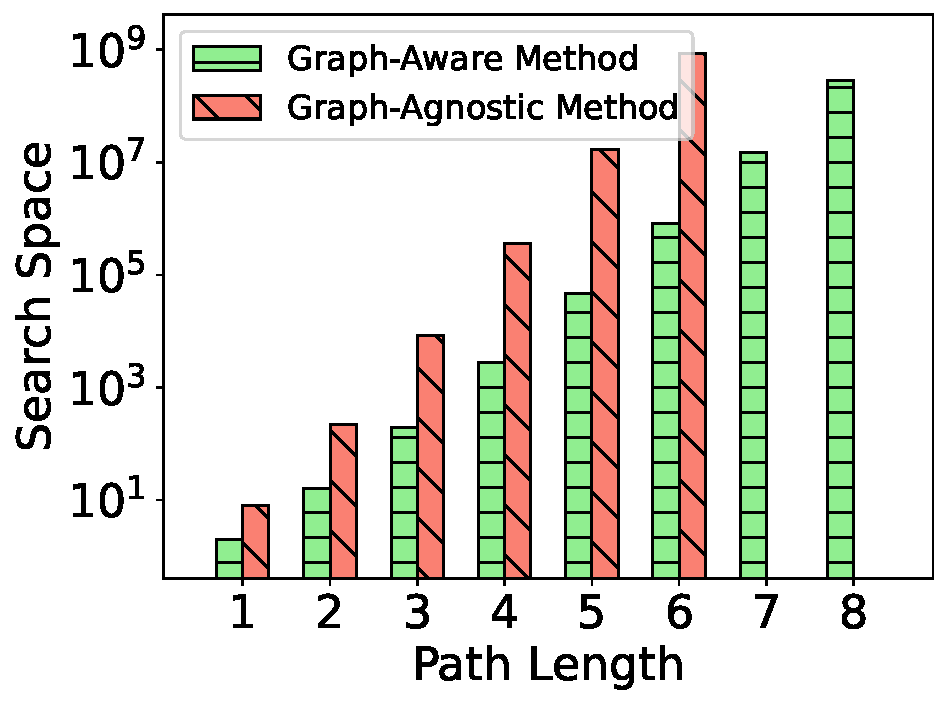
\includegraphics[width=\linewidth]{./figures/exp/compare_search_space.pdf}
        \end{subfigure}
        \begin{subfigure}[b]{0.45\linewidth}
            \centering
            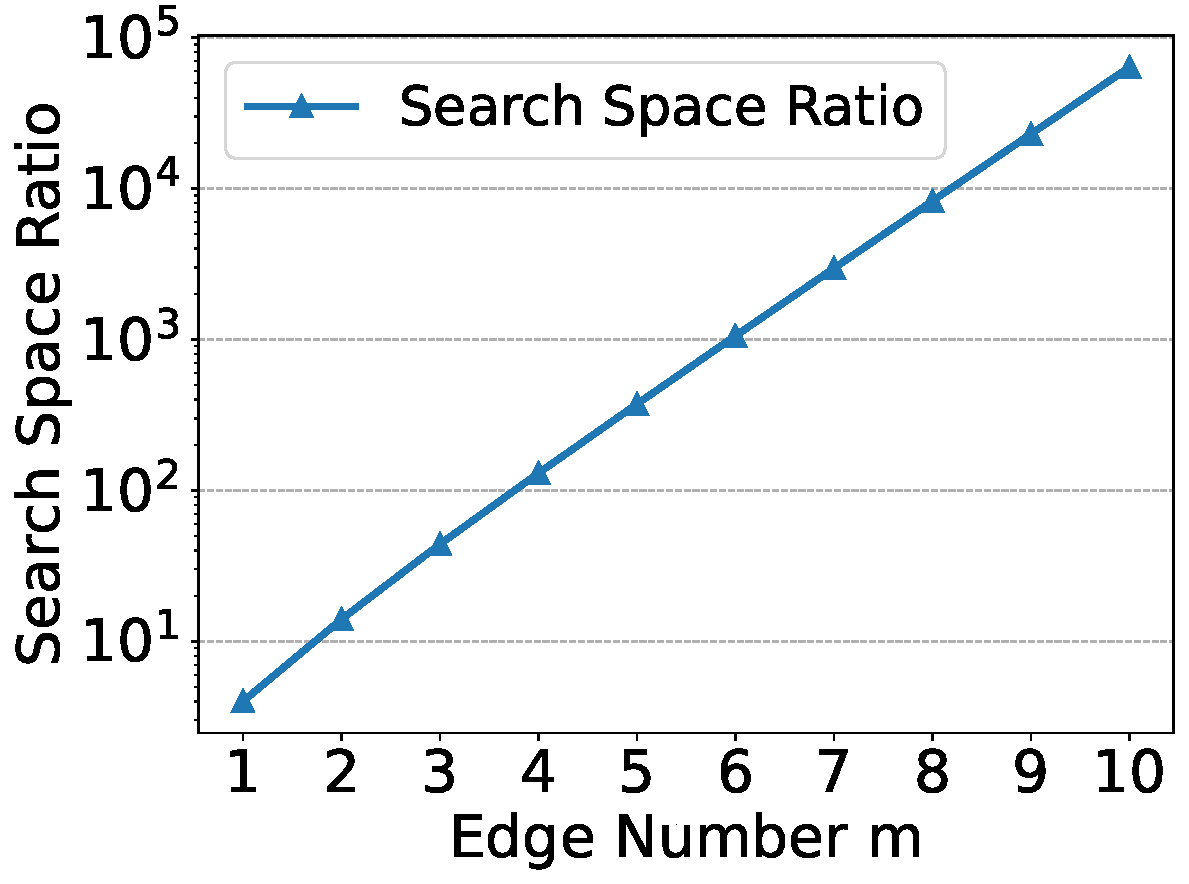
\includegraphics[width=\linewidth]{./figures/exp/compare_search_space_ratio.pdf}
        \end{subfigure}
        \caption{Search Space Comparison.}
        \label{fig:exp-search-space}
    \end{subfigure}
    \begin{subfigure}[b]{0.8\linewidth}
        \centering
        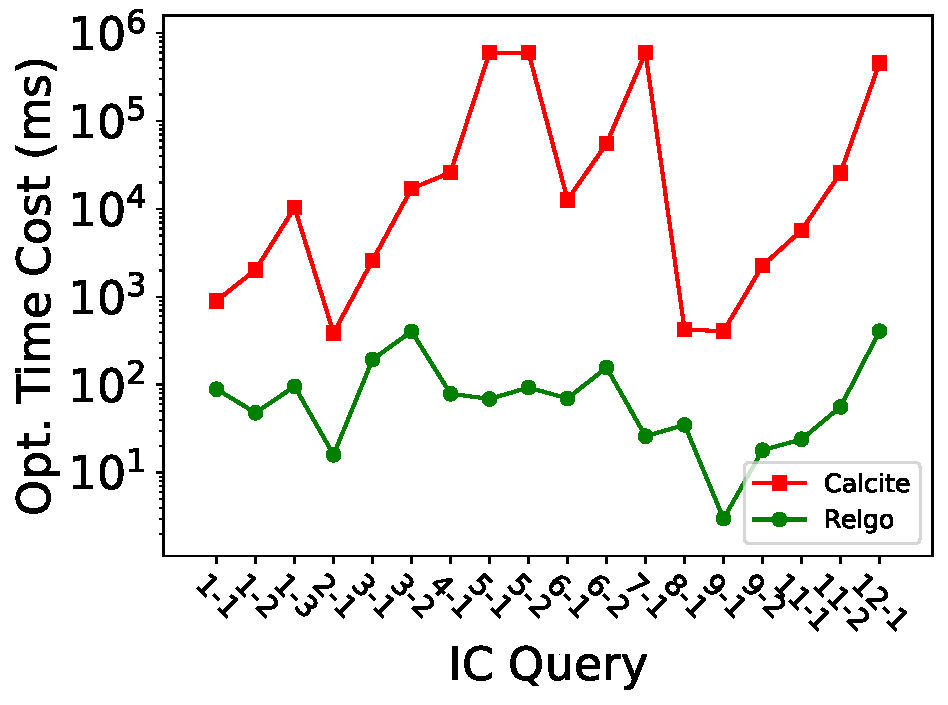
\includegraphics[width=\linewidth]{./figures/exp/optimization_sf30.pdf}
        \caption{Optimization Time Cost on $G_{sf30}$.}
        \label{fig:exp-optimization-sf30}
    \end{subfigure}
    \begin{subfigure}[b]{0.8\linewidth}
        \centering
        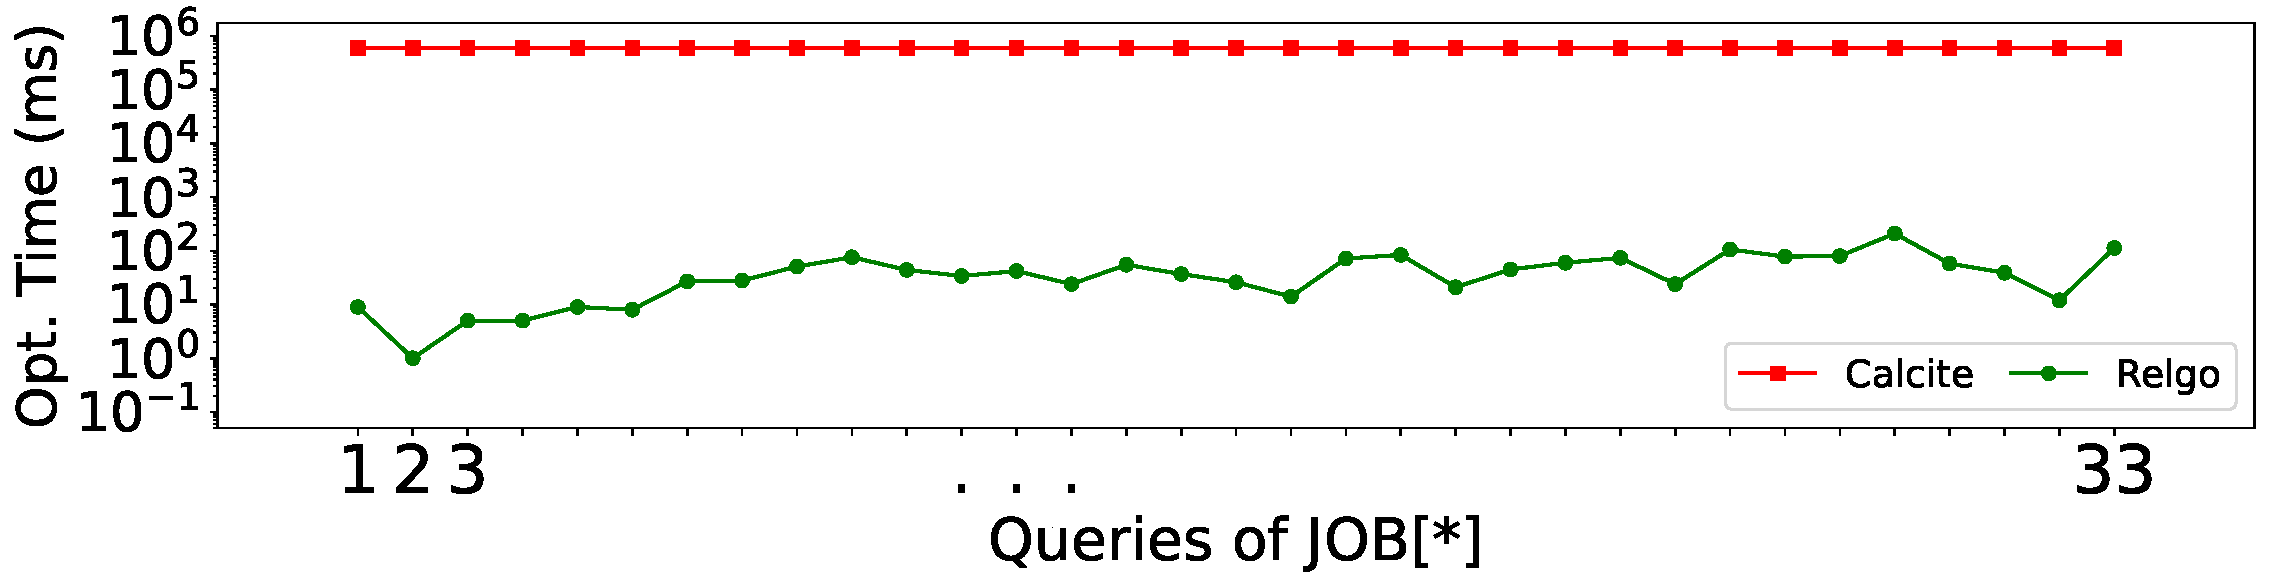
\includegraphics[width=\linewidth]{./figures/exp/optimization_job.pdf}
        \caption{Optimization Time Cost on IMDB.}
        \label{fig:exp-optimization-job}
    \end{subfigure}
    \caption{Experiments on the search space and time cost of optimization.}
    \label{fig:exp-optimization}
\end{figure}



%To verify the correctness of \refthm{compare-search-space}, we conduct corresponding experiments to test the size of the search space (i.e., the number of all possible physical plans or the number of decomposition trees) and the time required to traverse the entire search space when using the graph-agnostic method and the graph-aware Method.
%Specifically, we consider the case where the pattern in the matching operator consists of a path formed by $n+1$ nodes and $n$ edges.
%The experimental results are shown in \reffig{exp-compare-search-space-and-time}.



%\begin{figure}[ht]
%    \centering
%    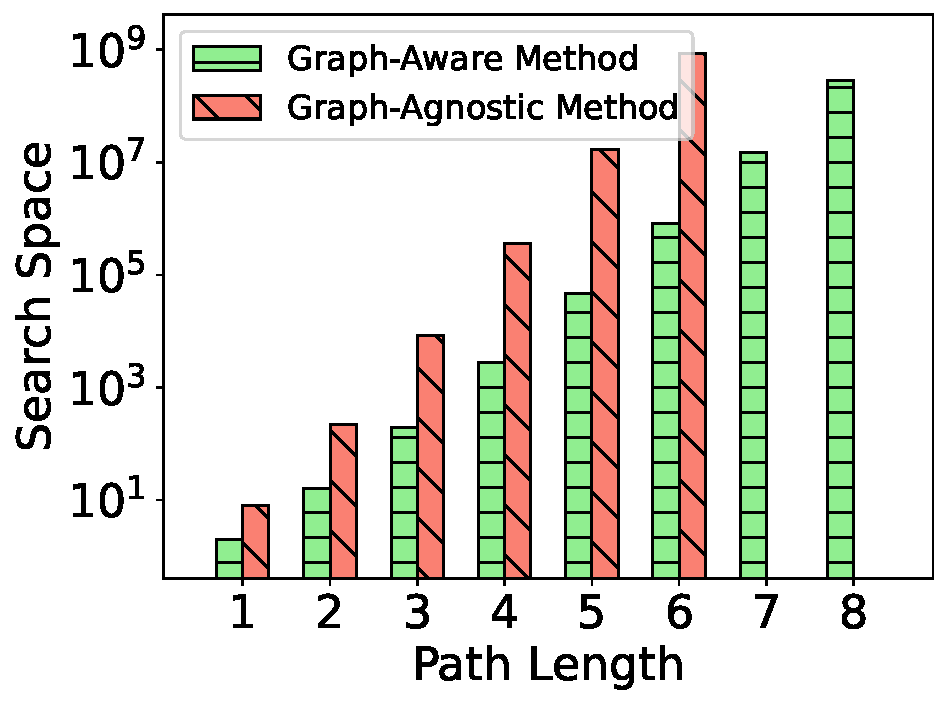
\includegraphics[width=.8\linewidth]{./figures/exp/compare_search_space.pdf}
%    \caption{Search Space Comparison.}
%    \label{fig:exp-search-space}
%\end{figure}

%Please note that when the path length is greater than 6, the memory usage of the graph-agnostic method exceeds the limit.
%\reffig{exp-compare-search-space-and-time} indicate that with the increase of the number of joined relations, the search space of the both methods increase exponentially, and it is consistent with \reflem{lem:complexity-of-volcano} and \reflem{complexity-of-graph-aware}.
%Specifically, the results also demonstrate that the search space of the graph-agnostic method increase exponentially faster than that of the graph-aware method, which corroborates the correctness of \refthm{compare-search-space}.


\subsection{Physical Implementation}
\label{sec:physical-operators}

In the graph view, given a vertex $v$, it is efficient to obtain its adjacent edges and vertices (i.e., neighbors). However, in the relational view, such adjacency relationships between vertices and edges are not directly stored in relations but must be computed via the \EVjoin operations (\refeq{ev-join}). While there are multiple ways to construct the graph view in the literature~\cite{gart,GRFusion}, we refer to the method introduced in GrainDB~\cite{graindb}, which is free from materializing the graph. This approach avoids the extra storage cost associated with graph materialization and ensures compatibility with the relational context,
Specifically, GrainDB introduces an indexing technique called pre-defined join to improve the performance of join operations. As the pre-defined join essentially materializes the adjacency relationships, we treat it as a \emph{graph index} in this work.


\begin{figure}[t]
    \centering
    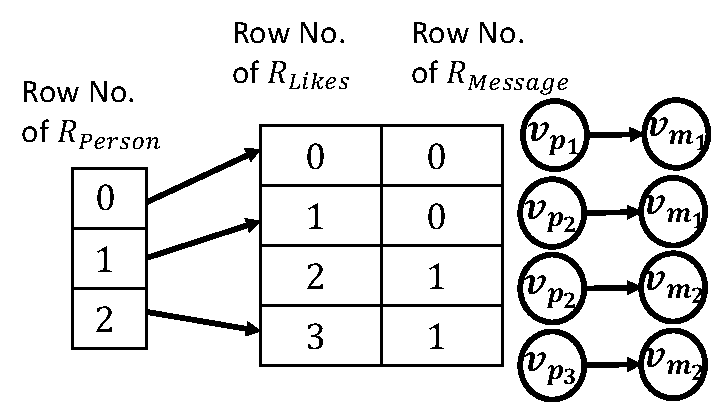
\includegraphics[width=.72\linewidth]{./figures/graph-index-likes.pdf}
    \caption{The graph index constructed among relations $\relation{\text{Person}}$, $\relation{\text{Likes}}$
    and $\relation{\text{Message}}$ in \reffig{intro-rgmapping-example}(a).}
    \label{fig:graph-index}
\end{figure}

\subsubsection{Graph Index}
\label{sec:graph-index}

As shown in \reffig{graph-index}, given the three relations $\relation{\text{Person}}$, $\relation{\text{Likes}}$, and $\relation{\text{Message}}$, the complete information of ``Person likes messages'' can be obtained by conducting the join:
\[ \relation{\text{Person}} \Join_\text{person\_id = pid} \relation{\text{Likes}} \Join_\text{mid = message\_id} \relation{\text{Message}}. \]

%\enlargethispage{1em}

GrainDB introduces two kinds of indexes to the relational tables to efficiently process the join: the EV-index and the VE-index. The EV-index, shown in \reffig{graph-index}(a), is constructed by appending extra columns to the table $\relation{\text{Likes}}$. The column ``\text{pid\_rowid}'' stores the row ID of the corresponding tuple in the table $\relation{\text{Person}}$, denoted as $\rowid(\tau_{p})$, where $\tau_{p} \in \relation{\text{Person}}$. Similarly, the column ``\text{mid\_rowid}'' stores the row ID of the corresponding tuple in the table $\relation{\text{Message}}$, denoted as $\rowid(\tau_{m})$, where $\tau_{m} \in \relation{\text{Message}}$. These row ids help quickly route a tuple $\tau_{l} \in \relation{\text{Likes}}$ to the joinable tuples $\tau_{p}$ and $\tau_{m}$ without additional operations like hash-table lookup or sorting.

The VE-index in \reffig{graph-index}(b) is created on $\relation{\text{Person}}$ for efficiently computing its ``liked messages''. For each tuple $\tau_{p} \in \relation{\text{Person}}$, the VE-index records the row ids of tuples $\tau_{l} \in \relation{\text{Likes}}$ and the corresponding $\tau_{m} \in \relation{\text{Message}}$ that are joinable with $\tau_{p}$. In the graph view, treating ``Person-[Likes]->Messages'' as an edge of a property graph, the VE-index maintains the adjacent edges and vertices of each person.
%GrainDB organizes the VE-index using the Compressed-Sparse-Row (CSR) structure that is widely used for maintain adjacency lists in graph store.

We can adopt GrainDB's approach to construct the graph indexes during the \rgmapping process. Given an edge relation $R_e$ and its associated vertex relations $R_{v_s}$ and $R_{v_t}$, the EV-index can be constructed on $R_e$ for each tuple $\tau_e \in R_e$ by including $\rowid(\lambda_e^s(\tau_e))$ and $\rowid(\lambda_e^t(\tau_e))$, which are the row ids of the corresponding tuples in $R_{v_s}$ and $R_{v_t}$, respectively. Meanwhile, the VE-index can be constructed on $R_{v_s}$ for each tuple $\tau_{v_s} \in R_{v_s}$ by including the row ids of all tuples $\tau_e \in R_e$ such that $\lambda_e^s(\tau_e) = \tau_{v_s}$, along with the row ids of the corresponding tuples $\tau_{v_t} \in R_{v_t}$ such that $\lambda_e^t(\tau_e) = \tau_{v_t}$.
The construction of VE-index on $R_{v_t}$ is analogous.

\comment{
\begin{remark}
  Several alternative approaches exist for handling the \rgmapping process. One such approach, proposed in~\cite{gart}, involves directly materializing the property graph using an additional graph store, rather than simply building graph indexes on the relational data. While this method may enable more efficient graph processing, it comes with the trade-off of requiring extra storage space and incurring higher maintenance costs. Moreover, \spjm queries often involve a combination of graph and relational operations, which may not be fully supported by the graph store alone.
\end{remark}
}

%With the graph indexes constructed, we can efficiently compute the \EVjoin operation in \refeq{ev-join}.
%When using the graph-agnostic method to transform the \spjm query into \spj, as shown in \refeq{graph-agnostic}, and optimizing the entire \spj query with a relational optimizer, we can replace all the \emph{remaining} \EVjoin operations with GrainDB's pre-defined joins. This allows us to take advantage of the graph indexes provided by GrainDB. We consider this approach as the baseline ``GrainDB'' solution in our experiments.
%However, as mentioned earlier, any pair of edge and vertex relations in an \EVjoin operation can be separated during the optimization process, preventing the utilization of graph indexes.
%\modify{In \refsec{experiment-opt}, we demonstrated through experiments that using this index can be about twice as fast compared to not using the index.}
%Even if certain rules are installed to prevent such separation, the resulting plan may still be suboptimal. This is because the plan for solving the matching operator reflects a naive method of edge-based join plan~\cite{lai2019distributed}, which is not worst-case optimal. \todo{add a few experiment findings}
%\modify{Specifically, experimental results in \reffig{exp-expand-intersect} indicate that the performance of a worst-case-optimal plan can be improved by about 1.3$\times$.}

\subsubsection{The Graph-Aware Execution Plan}
\label{sec:join-matching-operator}
We delve into the physical implementation of the execution plan provided by the graph-aware method for solving $\matching(\pattern)$. The entry point of the plan is always matching a single-vertex pattern $\pattern_u$, which is one of the leaf nodes in the decomposition tree.

%\enlargethispage{1em}

The implementation of $\matching(\pattern_u)$ is straightforward: scanning the corresponding vertex relation $\relation{\lab(u)}$ and encoding each tuple as a graph vertex object that contains its ID and label (mandatory) and necessary attributes. The row ID of the tuple in the relation can be directly used as the ID. To ensure globally uniqueness, the name of the relation can be incorporated as a prefix of the ID. Advanced encoding techniques are necessary for production use, but they are beyond the scope of this paper.

The plan is then constructed in a bottom-up manner. As shown in \reffig{match-decomposition}, there are three fundamental cases to consider when implementing the plan.

\stitle{Case I: Solving $\matching(\pattern') = \matching(\pattern'_l) \gjoin_{V_o, E_o} \matching(\pattern'_r)$}, where $\pattern_l'$ and $\pattern'_r$ are both intermediate patterns in the decomposition tree. The implementation of such a join is similar to a conventional relational join. The join is constrained to a natural join, where the join condition is simply the equality of the common vertices $V_o$ and edges $E_o$ between $\pattern_l'$ and $\pattern_r'$. During the implementation of the join, the identifiers of the vertices and edges can serve as the keys for comparison. Note that the input and output of the join are both graph relations, which will not
be projected into relational tuples until the last stage that obtains the results $\matching(\pattern)$.

\stitle{Case II: Solving $\matching(\pattern') = \matching(\pattern'_l) \gjoin_{u_s} \matching(\pattern_e)$}, where $\pattern_e$ is a single-edge pattern, and $u_s$ is the source vertex in $\pattern'_l$ from which the edge $e = (u_s, u_t)$ is expanded. Note that it's not possible for both $u_s$ and $u_t$ to be in $\pattern'_l$, as it would violate the fact that $\pattern'_l$ is either a single vertex or an induced sub-pattern.

\modify{When there is no graph index, $\matching(\pattern_e)$ is computed via $R_{\lab(u_s)} \evjoin R_{\lab(e)} \evjoin R_{\lab(u_t)}$}.
%where the first join is to obtain the edge tuples that connect $u_s$, which are encoded into edge objects,
%and the second join is to obtain the associated vertex tuples of $u_t$, which are encoded into vertex objects.
This case is then reduced to Case I. %, where a join operation is performed between $\matching(\pattern'_l)$ and the computed $\matching(\pattern_e)$.

When graph indexes exist, the implementation is handled by the physical operators of \expandedge~ and \getvertex. For each tuple $\tau \in \matching(\pattern'_l)$, $\tau.u_s$ must record a graph vertex $v_s$ that matches $u_s$ in the pattern $\pattern'_l$. The \expandedge~ operator looks up the VE-index of $v_s$, which allows it to efficiently computes $v_s$'s adjacent edges (more precisely, it's the corresponding edge tuples). Furthermore, the \getvertex~ operator is used to obtain the matched vertex $v_t$ that is connected to $v_s$ via the previous matched edges, which can be achieved by looking up the EV-index of the matched edges.
By combining the results of \expandedge~ and \getvertex, the tuple of $(\tau, \adj^E(v_s), \adj(v_s))$ is rendered. For example, in \reffig{graph-index}(b), if we apply \expandedge~ and \getvertex~ to a tuple $\tau$ from $v_{p_2}$, the result $(\tau, [e_{l_2}, e_{l_3}], [v_{m_1}, v_{m_2}])$ is returned.
Furthermore, to obtain $\matching(\pattern')$, we flatten the adjacent edges and vertices and pair them up. In the case of $(\tau, [e_{l_2}, e_{l_3}], [v_{m_1}, v_{m_2}])$, two tuples $(\tau, e_{l_2}, v_{m_1})$ and $(\tau, e_{l_3}, v_{m_2})$ are generated.

In real-life scenarios, a vertex may be adjacent to multiple types of edges. For example, in \reffig{intro-rgmapping-example}, a \kk{Person} vertex can be connected to both \kk{Likes} and \kk{Knows} edges. To handle such cases, we can record edge's ID instead of just the row ID of the tuple. Given that the edge's ID is a combination of its label and the tuple's row ID, the adjacent edges of a specific label can be easily obtained from the VE-Index.

\stitle{Case III: Solving $\matching(\pattern') = \matching(\pattern'_l) \gjoin_{V_s, E_s} \matching(\pattern(u;V_s))$}, where pattern $\pattern(u;V_s)$ is a complete $k$-star with $V_s = \{u_1, \ldots, u_k\}$. %In this case, $\pattern'_l$ is a sub-pattern, and $\pattern(u;V_s)$ is a complete $k$-star pattern with a root vertex $u$ and leaf vertices $V_s = \{u_1, \ldots, u_k\}$.

When there is no graph index, solving Case III involves continuously joining $|V_s|$ single-edge patterns.

When graph indexes are available, the \expandintersect~ operator can be used to efficiently compute the join. 
\revise{Unlike HUGE \cite{huge}, \expandintersect~ is implemented on a relational database}.
Given a tuple $\tau \in \matching(\pattern'_l)$, let $\{v_1, \ldots, v_k\}$ be the vertices in $\tau$ that match the leaf vertices $\{u_1, \ldots, u_k\}$ in the complete star $\pattern(u;V_s)$. The vertices that can match the root vertex $u$ of the star must be the common neighbors of all the leaf vertices.

Consequently, for the tuple $\tau$, the physical \expandintersect~ operator performs the following steps:

\comment{When graph indexes are available, the \expandintersect~ operator, introduced in the literature~\cite{huge,GLogS,mhedhbi2019optimizing}, can be used to efficiently compute the join. Given a tuple $\tau \in \matching(\pattern'_l)$, let $\{v_1, \ldots, v_k\}$ be the vertices in $\tau$ that match the leaf vertices $\{u_1, \ldots, u_k\}$ in the complete star $\pattern(u;V_s)$. The vertices that can match the root vertex $u$ of the star must be the common neighbors of all the leaf vertices.}

% Consequently, for the tuple $\tau$, the physical \expandintersect~ operator performs the following steps:

\begin{enumerate}
\item For each leaf vertex $u_i \in V_s$ ($1 \leq i \leq k$), apply the \expandedge~ \\ and \getvertex~ operators to obtain the adjacent edges and neighbors of the corresponding vertices $v_i$ respectively.
\item Compute the intersections of all adjacent edges and neighbors returned by the \expandedge~ and \getvertex~ operators.
\item Return a new tuple as follows; for the sake of simplicity, the details of the edges are omitted: $(\tau, \bigcap\limits_{1 \leq i \leq k}\adj(v_i))$.

%\[
%    \left(\tau,\bigcup\limits_{v_c \in \bigcap\limits_{1 \leq i \leq k} \adj(v_i)} (v_c, \bigcup\limits_{1 \leq i \leq k}\adj^E(v_i, v_c))\right)
%\]

\end{enumerate}

Note that the above step (1) and (2) can be computed in a pipeline manner, following a certain order of among the leaf vertices.
Similar to Case II, we flatten the common edges and vertices and pair them up to obtain the final result.


\begin{example}
    \label{ex:physical-implementation}
    Given $\pattern$ in \reffig{match-decomposition}, a decomposition tree and its corresponding logical plan are presented. We illustrate the physical implementation of $\matching(\pattern_1) \gjoin \matching(\pattern_2)$ using \expandintersect when a graph index is available.
    Consider the tuple $(v_{p_1}, e_{k_1}, v_{p_2})$ from $\matching(\pattern_1)$ as an example. First, the \expandedge~ and \getvertex~ operators are applied to obtain the adjacent edges and neighbors of $v_{p_1}$ and $v_{p_2}$, resulting in
    \begin{equation*}
        \begin{split}
    &(v_{p_1}, e_{k_1}, v_{p_2}, [e_{l_1}], [v_{m_1}]), \text{and} \\
    &(v_{p_1}, e_{k_1}, v_{p_2}, [e_{l_2}, e_{l_3}], [v_{m_1}, v_{m_2}]).
        \end{split}
    \end{equation*}
    Next, the intersection process is conducted. Since $\adj(v_{p_1}) \cap \adj(v_{p_2}) = [v_{m_1}]$, the edges in both sets that have $v_{m_1}$ as the target vertex are retained, resulting in $(v_{p_1}, e_{k_1}, v_{p_2}, [(e_{l_1}, e_{l_2}, v_{m_1})])$. Finally, the tuple is flattened to $(v_{p_1}, e_{k_1}, v_{p_2}, e_{l_1}, e_{l_2}, v_{m_1})$.

    \comment{
    Case II: $\matching(\pattern_3) \gjoin \matching(\pattern_4)$ is implemented using \expandedge~and \getvertex. Take $v_{p_1} \in \matching(\pattern_3)$ as an example, we first do \expandedge by looking up the
    VE-index corresponding to $v_{p_1}$ in \reffig{graph-index}(b), which
    locates the edge $e_{}$ the $0^{th}$ row of $\relation{\text{Likes}}$. Then, \getvertex~is computed by looking up the EV-index \reffig{graph-index}(a), which locates the vertex tuples corresponding to $v_{m_1}$

    is implemented and it pertains to Case II, since the $\pattern_6$ is a single-edge pattern.
    Thus, when there is no graph index on $\relation{Likes}$, the results of $\matching(\pattern_4)$ is computed via $\relation{Person} \Join_{person\_id = pid1} \relation{Knows} \Join_{pid2 = person\_id} \relation{Person}$.
    Specifically, the results include tuples $(v_{p_1}, e_{k_1}, v_{p_2})$, $(v_{p_2}, e_{k_2}$, $v_{p_1})$, $(v_{p_2}, e_{k_3}, v_{p_3})$, and $(v_{p_3}, e_{k_4}, v_{p_2})$.
    Then, since $\pattern_3$ is a single-vertex pattern whose vertex exists in $\pattern_4$, the results of the join equals $\matching(\pattern_4)$.
    Otherwise, if a graph index exists, $\matching(\pattern_4)$ can be computed with \expandedge~and \getvertex.
    }
\end{example}

\section{The Converged Optimization Framework}
\label{sec:optimizations}
%\enlargethispage{1em}
This section presents \name, a converged relational/graph optimization framework designed to optimize the query
processing of \spjm queries. We begin by introducing a naive solution built upon the graph-agnostic
method for solving the matching operator. We then delve into the converged workflow of \name, which leverages the graph-aware method for solving the matching operator and introduces a complete workflow that aims to integrate techniques from both relational and graph optimization modules.


%\begin{figure}
%    \centering
%    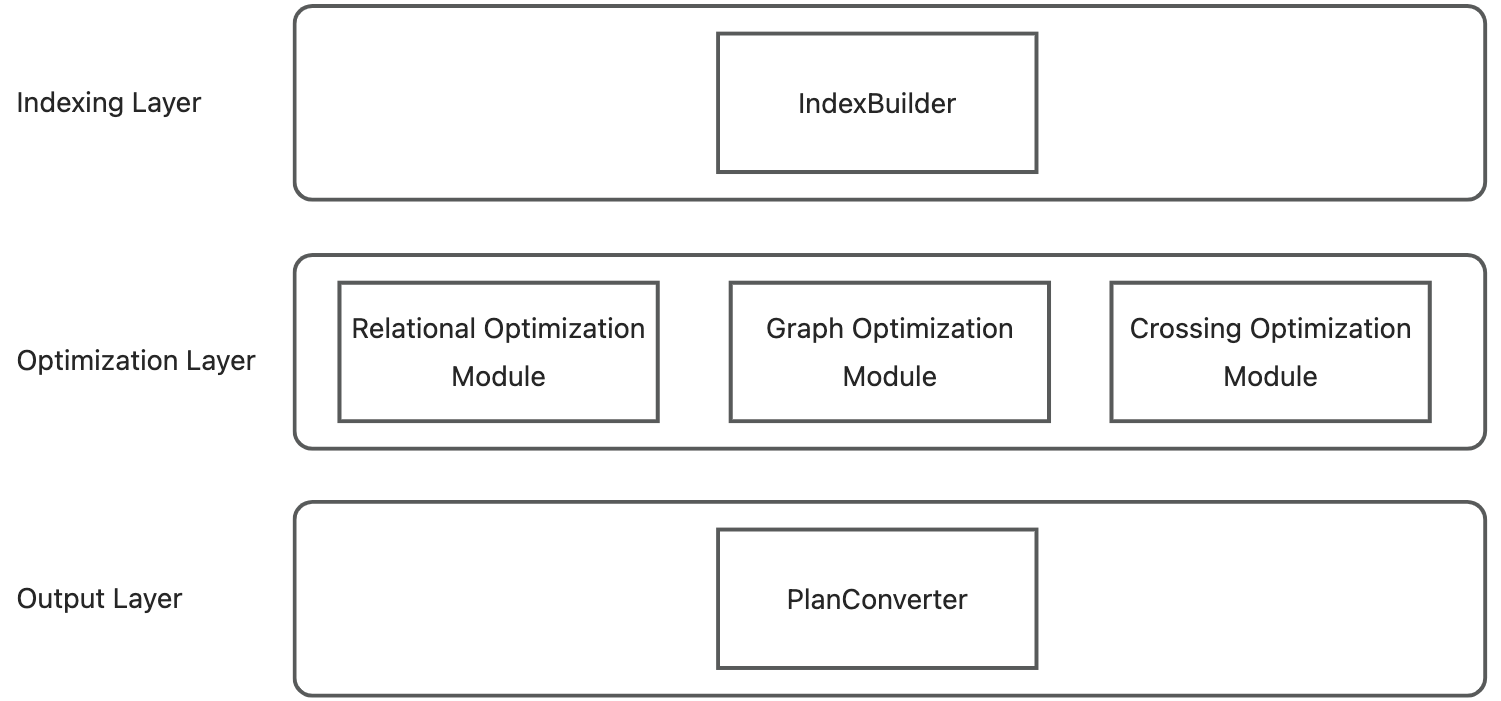
\includegraphics[width=\linewidth]{./figures/framework.png}
%    \caption{Overview of the Converged Graph Relational Optimization Framework.}
%    \label{fig:framework-overview}
%\end{figure}

\begin{figure*}
    \centering
    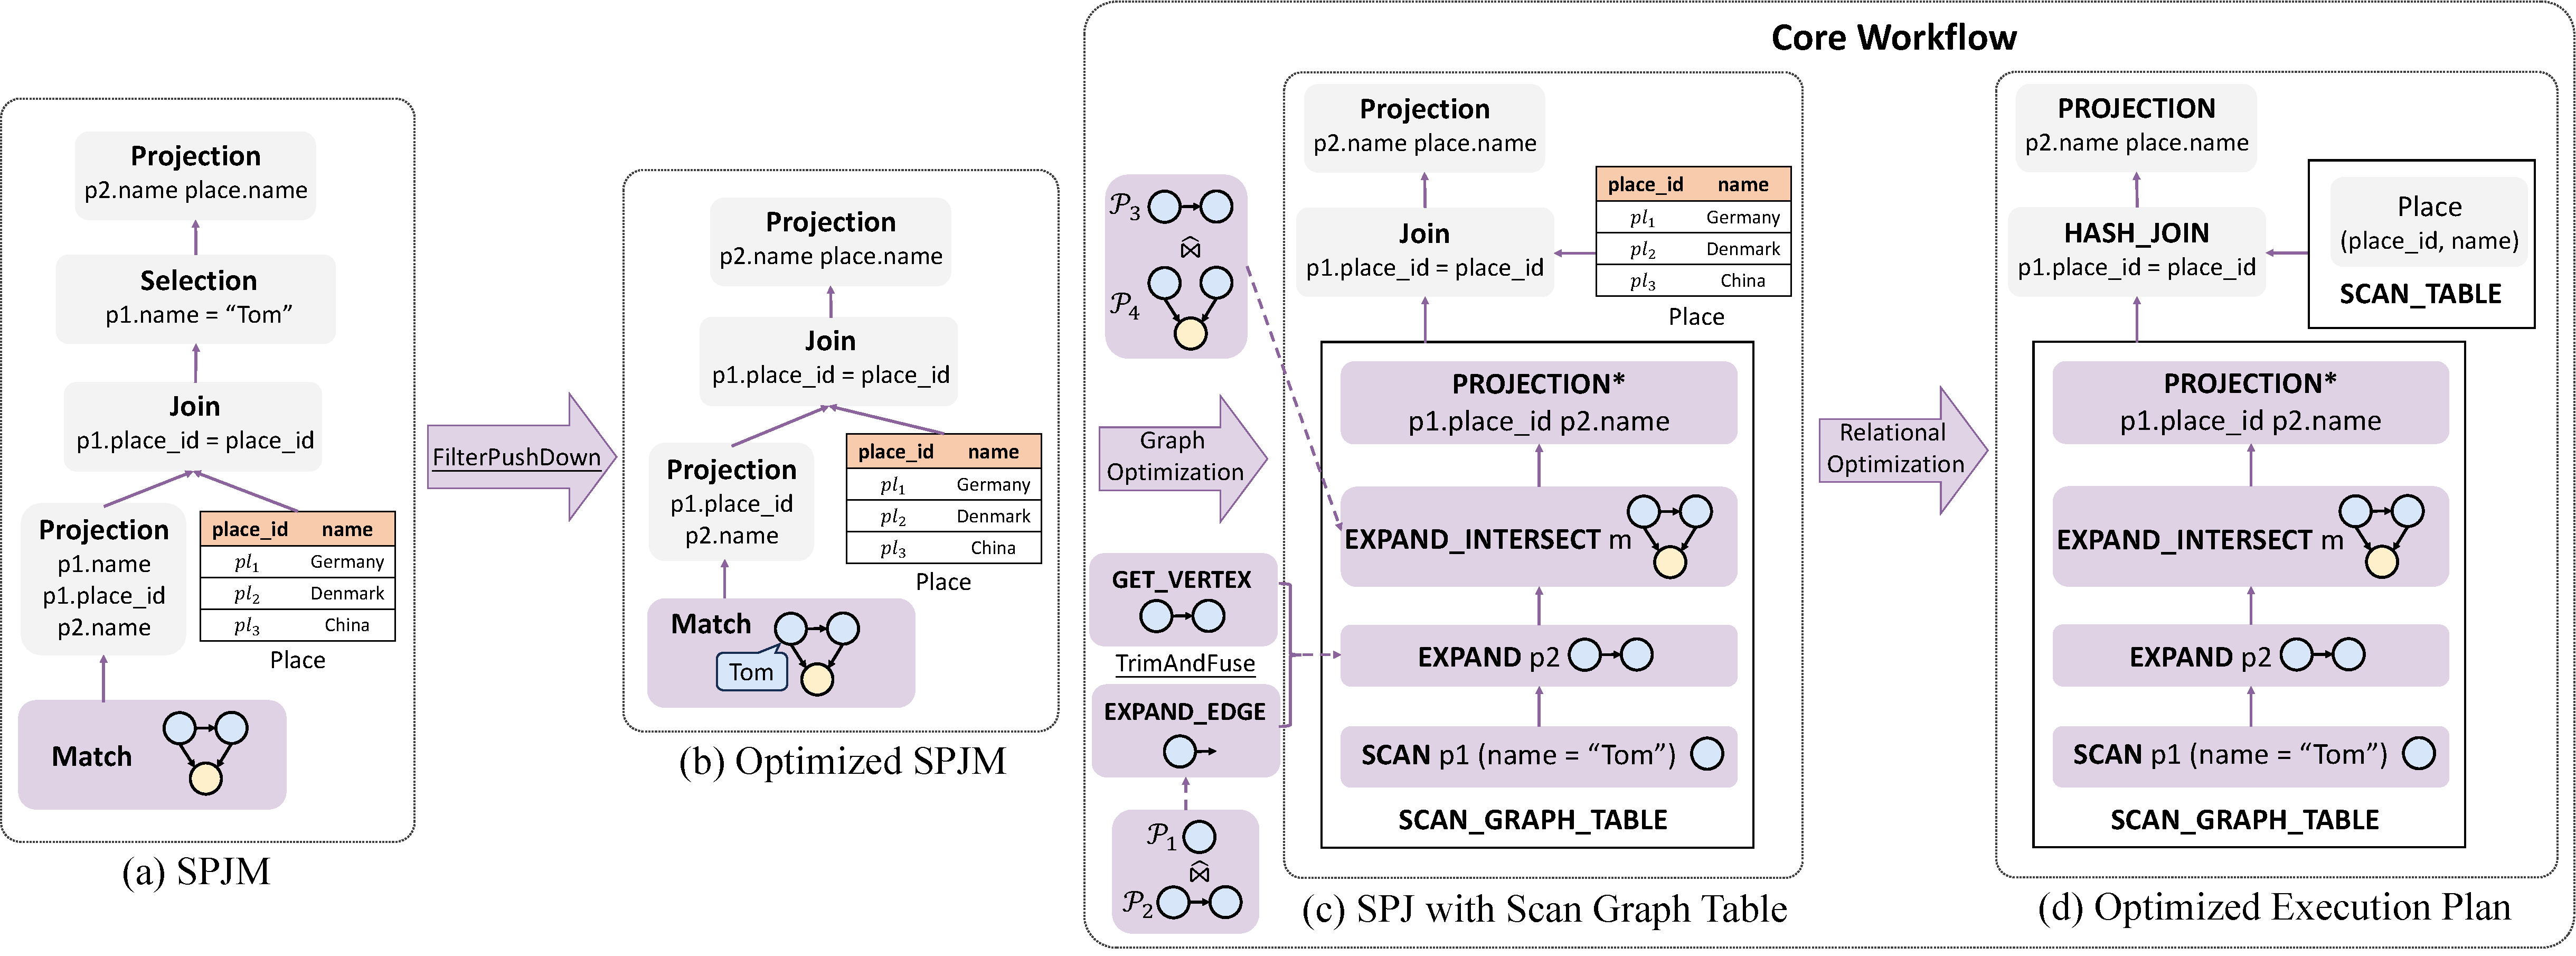
\includegraphics[width=.88\linewidth]{./figures/workflow.pdf}
    \caption{The converged optimization workflow}
    \label{fig:framework-workflow}
\end{figure*}


\vspace*{-3mm}
\subsection{Graph-Agnostic Approach}
\label{sec:relational-only}
The graph-agnostic approach is straightforward: it applies the graph-agnostic transformation for the matching operator in an \spjm query into a series of relational operations (\modify{\reflem{spjm-to-spj}}), effectively converting the \spjm query into an \spj query. The resulting \spj query can then be optimized by any existing relational optimizer, producing an execution plan. As an improvement, if a graph index (\refsec{graph-index}) is available, certain hash-join operators in the execution plan can be replaced by the predefined-join operator, as discussed in GRainDB~\cite{graindb}. The main advantage of this solution is its easy integration with any existing relational database. However, it suffers from two significant drawbacks discussed in \refrem{graph-agnostic-vs-graph-aware}.
%that have been discussed in \refrem{graph-agnostic-vs-graph-aware}.

\vspace*{-3mm}
\subsection{The Converged Approach}
\label{sec:converged}
As illustrated in \reffig{framework-workflow}, the core workflow of the \name framework consists of two components: \emph{graph optimization} and \emph{relational optimization}. The graph optimization is responsible for handling the graph component in an \spjm query, leveraging graph optimization techniques to determine the optimal decomposition tree of the matching operator. On the other hand, the relational optimization takes over to optimize the relational component in the query.
The order in which these two components are applied is not strictly defined. However, for the purpose of our discussion, we will first focus on the graph optimization and then proceed to the relational optimization.
In addition to the core workflow, we further explore heuristic rules that highlight the non-trivial interplay between the relational and graph components in an \spjm query.

 %our analysis of real-life querying scenarios has revealed the need for a \emph{preposition optimizer}. This component is applied prior to the core workflow and is designed to apply heuristic rules.

%In addition to the primary component, we finally demonstrate the necessity of applying a \emph{preposition optimizer} component prior to the primary component.

%\enlargethispage{1em}

\vspace*{-1mm}
\subsubsection{The Graph Optimization}
\label{sec:graph-optimizer}
We adopt the graph optimization techniques developed in \glogs~\cite{GLogS}. However, it is crucial to note that \glogs~ was originally designed for native graph data, whereas our framework deals with relational data, which necessitates a careful adaptation of \glogs's techniques to the relational setting.

\stitle{\glogue~Construction.} \glogs is built upon a data structure called \glogue, which is essentially a graph $\searchgraph_{\pattern}(V, E)$. In this graph, each vertex represents a pattern $\pattern'$ consisting of up to $k$ vertices (typically, $k=3$) that has non-empty matched instances in the original graph. There is an edge from $\pattern''$ to $\pattern'$, if there is a decomposition tree where $\pattern''$ is a child node of $\pattern'$.

 Each vertex $\pattern'$ in \glogue maintains $|\matching(\pattern')|$, denoting the cardinality of the pattern. To reduce computation costs, \glogs employs a sparsification technique to construct a subgraph $G'$. The pattern cardinality can then be estimated using $|\matching_{G'}(\pattern')|$ based on subgraph $G'$. In our work, we adapt this sparsification technique to construct \glogue. We sample a subset of vertex and edge relations in the \rgmapping process. Once the subset of relations is obtained, they can serve as the input tables to the techniques presented in~\cite{gart} for constructing the sparsified graph $G'$.

 %\enlargethispage{1em}

\stitle{Cost Calculation.} The optimization process is essentially searching for the execution plan that incurs the minimal cost. Let the cost of an execution plan $\Phi$ for computing $\matching(\pattern)$ be $\cost_\Phi(\pattern)$. %The graph optimizer aims to find an optimal execution plan such that $\cost_\Phi(\pattern)$ is minimized. Clearly, this can be solved using dynamic programming~\cite{GLogS}.

Consider $\matching(\pattern') = \matching(\pattern'_l) \gjoin \matching(\pattern'_r)$ as an intermediate computation in an execution plan. We have:
\[
\cost_{\Phi}(\pattern') = \cost_{\Phi_l}(\pattern'_l) + \cost_{\Phi_r}(\pattern'_r) + \cost(\gjoin),
\]
where $\Phi_l$ and $\Phi_r$ are the execution plans for computing $\matching(\pattern'_l)$ and $\matching(\pattern'_r)$, respectively, and $\cost(\gjoin)$ is the cost of the join operation.

When a graph index is available, there are three physical implementations of $\gjoin$, depending on the type of $\pattern'_r$, and the calculation of $\cost(\gjoin)$ differs accordingly:
\begin{itemize}
\item If $\pattern'_r$ is a single-edge pattern, $\gjoin$ is implemented using the \expandedge~ operator followed by \getvertex. The cost is calculated based on the cardinality of $\matching(\pattern'_l)$ (can be looked up in the \glogue) and the average degree of the graph, namely $|\matching(\pattern'_l)| \times \overline{d}$.
\item If $\pattern'_r$ is a complete star pattern, $\gjoin$ is implemented using the \expandintersect~ operator. The cost is calculated based on the cardinality of $\matching(\pattern'_l)$ and the average intersection size of the neighbors of the vertices being intersected, which is maintained on the corresponding edge from $P'$ to $\pattern'_l$ in \glogue.
\item  If $\pattern'_r$ is any arbitrary pattern, $\gjoin$ is implemented as a \hashjoin. The cost is calculated as the product of the cardinalities of the two relations being joined, i.e., $\cost(\gjoin) = |\matching(\pattern'_l)| \times |\matching(\pattern'_r)|$.
\end{itemize}

\revise{In the absence of a graph index, \hashjoin~ is used for the entire plan of the matching operator for simplicity, and its cost is computed as the product of the cardinalities of the two relations being joined. Although other physical join implementations, such as nested loop join, may be more effective if the join condition is not selective, considering these alternatives is planned for future work.}

%when we are dealing
%with the matching operators, the joins obtained by decompostion
%are implemented as HASH_JOINs. As these joins connect vertices
%to their adjacent edges, it is always far from cross product.

\comment{
\begin{example}
    As shown in \reffig{framework-workflow}, since $\matching(\pattern_2)$ is a single-edge pattern, the join operator between $\matching(\pattern_1)$ and $\matching(\pattern_2)$ is implemented using \expandedge~followed by \getvertex.
    Besides, as $\matching(\pattern_4)$ is a complete star, the join operator between $\matching(\pattern_3)$ and $\matching(\pattern_4)$ is implemented using the \expandintersect~operator.
\end{example}
}

\stitle{Plan Computation.} Searching for the optimal execution plan in \name remains the same as in \glogs. The optimal plan is obtained by searching for the shortest path in the \glogue from the single-vertex pattern to the queried pattern.  %The process is repeated until the $\pattern$ node is reached, at which point the optimal execution plan is obtained.
\reffig{framework-workflow}(c) demonstrates a physical plan for matching the given triangle pattern when a graph index is present. The plan reflects the example in~\refex{physical-implementation}, with one exception: the pair of \expandedge~ and \getvertex~ operators is fused into a single \expand~ operator, which will be discussed as a heuristic rule called \joinfuserule.


\subsubsection{The Relational Optimization}
Once the graph optimizer has computed the optimal execution plan for $\matching(\pattern)$, the next step is to integrate this plan with the remaining relational operators in the \spjm query. The relational optimization is responsible for optimizing these remaining operators, which are all relational operators.
\revise{Relational optimization has evolved into a well-established field, producing numerous significant results \cite{Chaudhuri98, Haffnerjoinorder}. Since existing relational optimization techniques can be seamlessly integrated into \name, we will focus on how graph optimization techniques can be applied to enhance relational queries.}
%Any existing relational optimizer can be used for this purpose.

%It's important to note that before $\matching(\pattern)$ can be integrated with the remaining relational component of the query, a specialized projection operator $\gproject$ must be applied to the matched results to flatten the graph relation into a relation, making it compatible with the relational operators. To facilitate this integration, we introduce a new physical operator called \scangraphtable, as shown in \reffig{framework-workflow}(c), which encapsulates the $\gproject$ operator and the optimal execution plan for $\matching(\pattern)$.

Specifically, to prevent the relational optimizer delve into the internal details of the graph pattern matching process, we introduce a new physical operator called \scangraphtable, as shown in \reffig{framework-workflow}(c), which encapsulates the $\gproject$ operator and the optimal execution plan for $\matching(\pattern)$.
The \scangraphtable~ operator acts as a bridge between the graph and relational components of the query. From the perspective of the relational optimizer, \scangraphtable~ behaves like a standard \scan~ operator, providing a relational interface to the matched results. %This abstraction allows the relational optimizer to treat \scangraphtable~ as a regular relational operator, without the need to delve into the internal details of the graph pattern matching process.

\subsubsection{Heuristic Optimization Rules}
In real-life use cases, heuristic rules may involve non-trivial interactions between the relational and graph components of an \spjm query. We explore two representative rules, \filterrule~ and \joinfuserule, which can be applied at different stages of the optimization process to improve query performance.


\stitle{\filterrule.} To elaborate the rule, we extend the definition of a pattern $(\pattern, \constraints)$, introducing constraints within $\constraints$. For example, constraints can specify predicate $d$ such as $\id(v_1) = p_1$ for a vertex $v_1$, or $e_1.date > \text{"2024-03-31"}$ for an edge $e_1$. With the constraints defined, any matching result of $\pattern$ must have the corresponding vertices and edges adhering to the predicates.

%\enlargethispage{1em}

While writing queries, users may not specify constraints on the pattern but rather use the selection operator after matching results have been projected into the relational relation, described as:
\[
\sigma_{d'_{v_a}} (\widehat{\pi}_{v.a \rightarrow \text{v\_a}, \ldots} \matching(\pattern))
\]
The predicate $d'_{v_a}$ defines a predicate in terms of an attribute of the pattern vertex that is projected by $\widehat{\pi}$ from the matched results. The motivation example in \refex{introduction:sqlpgq} illustrates such a case, where the selection predicate \kk{g.p1\_name = ``Tom''} is applied to the pattern vertex $v_{p_1}$.
There is wasteful computation if the selection is applied after the costly pattern matching. A more efficient approach is to push the selection predicate down into the matching operator.
%An extra benefit of doing so is that the optimizer can leverage the constraints to recalculate the cost, potentially generating better execution plans.
The \filterrule is formally defined as:
\begin{equation*}
\sigma_{\constraints} (\widehat{\pi}_{v.a \rightarrow \text{v\_a}, \ldots} \matching(\pattern)) \\
\equiv \sigma_{\constraints'} (\widehat{\pi}_{v.a \rightarrow \text{v\_a}, \ldots} \matching((\pattern, \{d_v\}))),
\end{equation*}
where $\constraints' = \constraints \setminus \{d'_{v_a}\}$, and $\{d_v\}$ is the corresponding constraints that are appended to the pattern $\pattern$.

It is recommended to apply the \filterrule before graph optimization, as this allows the optimizer to leverage the pushed-down constraints to recalculate the cost, potentially generating more efficient execution plans. \reffig{framework-workflow}(b) showcases the effects of applying the \filterrule, where the selection predicate \kk{g.p1\_name = ``Tom''} is pushed down into the matching operator.

\stitle{\joinfuserule.}
The \joinfuserule~ amis to streamline a query plan by merging the \expandedge~ and \getvertex~ operators which are commonly coupled in the implementation of matching operations, into a single \expand~ operator that retrieves the neighboring vertices directly.
However, such a fusion is permissible solely when the output edges by \expandedge~ are deemed unnecessary, so this rule further incorporates a preceded field trim step.
Specifically, the field trimmer would examine whether any subsequent relational processes rely on these edges, such as utilizing them for property projections or for filtering based on their attributes.
If no such operations are found, the edges can be trimmed.
Furthermore, the field trimmer would also consider a special case that the edges might be projected in the \scangraphtable~ operator as part of the matching results, but are subsequently unused in relational operations. In such cases, the edges can be trimmed as well.
After the field trim step, if the output edges are trimmed, the \expandedge~ operator can be fused with the \getvertex~ operator to form a single \expand~ operator, which can directly retrieve the neighboring vertices efficiently by looking up the VE-index of the source vertex when the graph index is available.

%
% The \joinfuserule~ aims to optimize the query plan by fusing \expandedge, which expands edges, and \getvertex, which retrieves the associated vertices, into a single \expand, which retrieves the neighboring vertices directly, to enhance the plan's efficiency.
% However, the fusion logical is not universally applicable, but relies on a preceded exam-and-trim procedure to determine whether the properties of the output vertices and edges are essential.
% For example, if subsequent relational operations do not require any vertex properties output by \getvertex~ (e.g., no property projection or filtering), the vertex properties can be trimmed.
% In this case, the \expandedge~ can be fused with the \getvertex~ to form a single \expand~ operator, and this fusion helps to eliminate the unnecessary join operation between the edge table and the associated vertex table to find the neighboring vertices, since the associated vertex ids (and labels) are already available in the adjacent edge table.
% Similarly, if the edge properties output by \expandedge~ are not required, it further optimize the fused \expand~ operation (with no edge properties required) by retrieving the neighboring vertices directly when the graph indices are available, which further eliminates the unnecessary join operation with the adjacent edge table.

%\enlargethispage{1em}

Note \revise{that \filterrule is actually a global optimization rule because there are cases where pushing the predicate into the matching operator does not always yield better plans. 
For instance, given $\matching(\pattern)$ and assuming the query represented by $\pattern$ is}
\begin{lstlisting}
    (v1:Person)-[:Knows]->(v2:Person)-[:Knows]->(v3:Person),
\end{lstlisting}
\revise{with the return values being the names of $v_1$, $v_2$, and $v_3$, and an additional constraint on $v_2$'s place\_id specified outside the matching operator.
If the predicate is pushed, then the first expansion to $v_2$ in the generated plan would require fetching all necessary properties. When the predicate's filtering capability is weak, this leads to additional overhead. However, if the predicate is not pushed, properties can be deferred, being retrieved only at the end of the plan. Therefore, it is necessary to specifically determine whether to push down the predicate}.
However, since it is mostly effective, we greedily apply \filterrule in the current version. A more comprehensive evaluation of this rule will be conducted in future work. 

On the other hand, \joinfuserule is a local optimization rule specifically designed for graph optimization. The effectiveness of these two rules is validated in \refsec{experiment-opt}. Our \name framework is designed to be generic, allowing different optimization rules to be easily integrated. %In addition to these simple yet effective rules, we have also designed several other rules, such as \degreerule, which avoids the final join for aggregate operations, and \subtaskremoverule, which converts some WHERE conditions to anti-joins and semi-joins} {\color{red} Robin: an extra rule can be explained with sufficient details}.

\vspace*{-2mm}
\subsection{System Implementation}
We engineered the frontend of \name in Java and built it upon Apache Calcite~\cite{calcite}
%, a widely used open-source framework for data management,
to utilize its robust relational query optimization infrastructure.
%The frontend of \name is responsible for parsing the input \spjm query, constructing the logical plan, and invoking the graph and relational optimizers to generate the optimal physical plan.
Firstly, we enhanced Calcite's SQL parser to recognize SQL/PGQ extensions, specifically to parse the \lstinline{GRAPH_TABLE} clause.
We created a new \lstinline{ScanGraphTableRelNode} that inherits from Calcite's core \lstinline{RelNode} class, translating the \lstinline{GRAPH_TABLE} clause into this newly defined operator within the logical plan.
Following the formation of the logical plan, the frontend invokes the converged optimizer to generate the optimal physical plan.
For the relational-graph interplay optimizations, we incorporate heuristic rules such as \filterrule and \joinfuserule into Calcite's rule-based HepPlanner, by specifying the activation conditions and consequent transformations of each rule.
For more nuanced optimization, we rely on the VolcanoPlanner, the cost-based planner in Calcite, to optimize the \lstinline{ScanGraphTableRelNode}.
We devised a top-down search algorithm that assesses the most efficient physical plan based on a cost model outlined in \refsec{graph-optimizer}, combined with high-order statistics from \glogue for more accurate cost estimation.
\revise{
    While low-order statistics primarily focus on the cardinalities of relational tables, high-order statistics also include the frequencies of sub-patterns (can be seen as the joined results of multiple tables of vertices and edges), which aids in more accurate cost estimation. It is important to note that \name remains functional with only low-order statistics, but the efficiency of the generated plan may decrease due to less accurate cost estimation.
}

For the remaining relational operators in the query, we leverage Calcite's built-in optimizer, which already includes comprehensive relational optimization techniques.
Lastly, the converged optimizer outputs an optimized and platform-independent plan formatted with Google Protocol Buffers (protobuf) \cite{protobuf}, ensuring the adaptability of \name's output to various backend database systems.
%. This ensures the adaptability of the \name framework's output to a variety of backend database systems.

We developed the \name framework's backend in C++ using DuckDB as the relational execution engine to showcase its optimization capabilities.
We integrated graph index support in GRainDB~\cite{graindb}. %, by building graph indices for predefined joins, as well as optimized sip join and merge sip join implementations (\todo{what is this}), leveraging the graph indices to speed up the execution, following the designs used in GRainDB~\cite{graindb}.
%Note we choose DuckDB instead of GRainDB directly as the backend, because DuckDB is more mature and incorporates advanced optimization techniques that are not yet available in GRainDB.
%However, we did bring in optimization features similar to those found in GRainDB to ensure that \name can take full advantage of the graph indices.
With graph index, the \expand, \expandedge~ and \getvertex~ operators can be optimized by directly using the predefined join in GRainDB.
Note that we craft a new join on DuckDB called \emph{EI-Join} for the support of \expandintersect.
Without graph index, the \hashjoin~ operator is used throughout the entire plan.
To execute the optimized plans within DuckDB, we introduced a runtime module that translates the optimized physical plan into a sequence of DuckDB/GRainDB-compatible executable operators.
%For instance, the \expand~ operator is materialized using the merge sip join implementation, which significantly benefits from graph indices for processing efficiency.
%Moreover, for the \intersect~ operator, we crafted a new worst-case-optimal join implementation, which achieves better performance compared to the traditional multiple join that is not worst-case optimal in DuckDB.
This runtime module essentially bridges the gap between the optimized plans produced by \name and DuckDB's execution engine, thereby validating \name's practicality and potential performance improvements for \spjm queries on an established relational database system.



% The \name system consists of three main components: the Metadata Provider, the Converged Optimizer, and the Plan Converter.
% The Metadata Provider maintains the metadata of the database, such as the schema information, the graph index information, and the statistics of the data.
% Specifically, we incorporated \glogue as a high-order statistics provider, which precomputed the small patterns with size up to $k$ (usually $k=3$) together with their cardinalities, for a more accurate cost estimation of the matching operator.
%This pre-computation are based on the sampled subsets of vertex and edge relations from the database, which are further constructed into a sparsified graph.

\comment{
In the Converged Optimizer,
we incorporated both graph optimization techniques and relational optimization techniques, to optimize the \spjm queries in a converged manner.
We use the rule-based optimization planner named HepPlanner in Calcite, to plug in heuristic optimization rules like \filterrule and \joinfuserule. We set up each rule by specifying the conditions under which it activates and the actions it takes once those conditions are met.
For more nuanced optimization, we employ the VolcanoPlanner, a cost-based optimization planner provided by Calcite, to optimize the match operator in a cost-based manner.
We have crafted a top-down search algorithm that calculates the most efficient physical plan for the match operator, leveraging the cost model outlined in \refsec{graph-optimizer}. The algorithm is informed by advanced statistics obtained from the Metadata Provider, ensuring a more precise cost estimation.
For the relational part, Calcite's built-in optimizer, which already includes comprehensive relational optimization techniques, is leveraged to fine-tune the rest of the relational operators in the query.
The Converged Optimizer generates its output as a unified plan formatted with Google Protocol Buffers (protobuf)\cite{protobuf}. This serialization format is both platform-independent and highly interoperable, facilitating the easy conversion of the unified plan into executable query plans tailored for the destination database system.
}
%To showcase the capabilities of the \name framework, we devised a Plan Converter that employs code generation techniques. This Plan Converter is adept at transforming the unified plan, produced by the Converged Optimizer, into executable code compatible with GRainDB, a relational database system that incorporates support for graph indices. This step is crucial in demonstrating the practical applicability and effectiveness of the \name framework in optimizing \spjm queries on a real-world relational database system.

\comment{
To optimize SPJM queries, we propose the converged graph relational optimization framework named relgo.
Specifically, optimizing SPJM queries with relgo is divided into three stages, i.e., preprocessing, optimizing, and converting.
In this section, we introduce the three stages of relgo in detail.

\subsection{Preprocessing Stage}
Given an SPJM query, relgo first parse the query and obtained the corresponding AST (Abstract Syntax Tree).
Then, the initial logical plan is obtained based on the AST.
Each node in the logical plan represents an operator, including the selection, projection, join, and scan operators.

Please note that the matching operator does not appear in logical plans, because it can be further decomposed into other operators such as join and selection operators.
Besides, according to \refdef{matching}, the output of the matching operator is a graph relation, and it is always followed by a projection operator $\widehat{\pi}$.
The output of $\widehat{\pi}$ is a relation and the matching operator as well as $\widehat{\pi}$ are considered as a whole as an implementation of the scan operator (named ScanMatchTable).

In the preprocessing stage, some universally effective optimizations can be applied to refine the plan in advance.
A typical optimization is \filterrule.

This rule is inspired by FilterPushdownRule in relational optimizer, which can push down the predicates to the scan operators to filter out invalid elements earlier.
Specifically, as the ScanMatchTable corresponding to $\matching(\pattern)$ is a physical implementation of the scan operator which acts like scanning a table obtained by matching $\pattern$, it is reasonable to integrate some filtering criteria into the ScanMatchTable operator.
Specifically, \filterrule finds predicates on the properties of elements in $\pattern$ and push them down into ScanMatchTable, so that invalid elements can be dropped earlier.
An example of applying \filterrule is given in Example \ref{example:push_down}.

Formally, the equation rule w.r.t.~\filterrule is as follows:
\begin{equation}
    \begin{split}
        & \pi_A(\sigma_{d}(R_1 \Join \cdots \Join R_m \Join \widetilde{R}) \\
        & \hspace*{2em} \equiv \pi_A(\sigma_{d_0}(R_1 \Join \cdots \Join R_m \Join \widetilde{R}_{d_1})), \\
        & \hspace*{4em} \text{where } \widetilde{R} = \widehat{\pi}_{attr*}(\mathcal{M}(\mathcal{P})) \\
        & \hspace*{4em} \text{and } \widetilde{R}_{d_1} = \widehat{\pi}_{attr*}(\mathcal{M}(\mathcal{P}_{d_1}))
    \end{split}
\end{equation}
where $d_1$ is a subset of $d$ with the constraints related to $\widetilde{R}$ and $d_0$ is obtained by removing $d_1$ from $d$.
Besides, $\mathcal{P}_{d_1}$ is obtained by adding constraints in $d_1$ to $\mathcal{P}$.

\subsection{Optimizing Stage}

Given a logical plan of a SPJM query, relgo optimizes the plan in the optimizing stage.
Specifically, the operations that appear in logical plans of SPJM queries often also appear in the logical plans of relational databases.
Therefore, typical relational optimizers, e.g., Calcite \cite{calcite}, can be employed to optimize this plan.

Besides, to optimize the implementation of ScanMatchTable, the matching plans are optimized with graph-aware methods.
Studies that optimize graph pattern matching can be utilized as the graph-aware methods, and when implementing \name, we leverage GLogS \cite{GLogS} to optimize matching plans.
Moreover, if graph indices are available, join operators in \expandvertex and \expandintersect can be implemented as predefined joins to further improve the efficiency.


\subsection{Converting Stage}

As different databases usually support different operators and their physical plans can be greatly varied, it is of critical importance for an optimization framework to be flexible.
Therefore, we implement a PlanConverter in the framework to ensure the flexibility.
Given the generated optimal physical plan, the PlanConverter transforms the plan to an internal representation (e.g., Substrait \cite{substrait}), and then the internal representation is transformed to the physical plan that can be executed by the target database.
Finally, the plan is executed and the query results are obtained.


The introduction of the framework is concluded with an example.


\begin{figure}
    \centering
    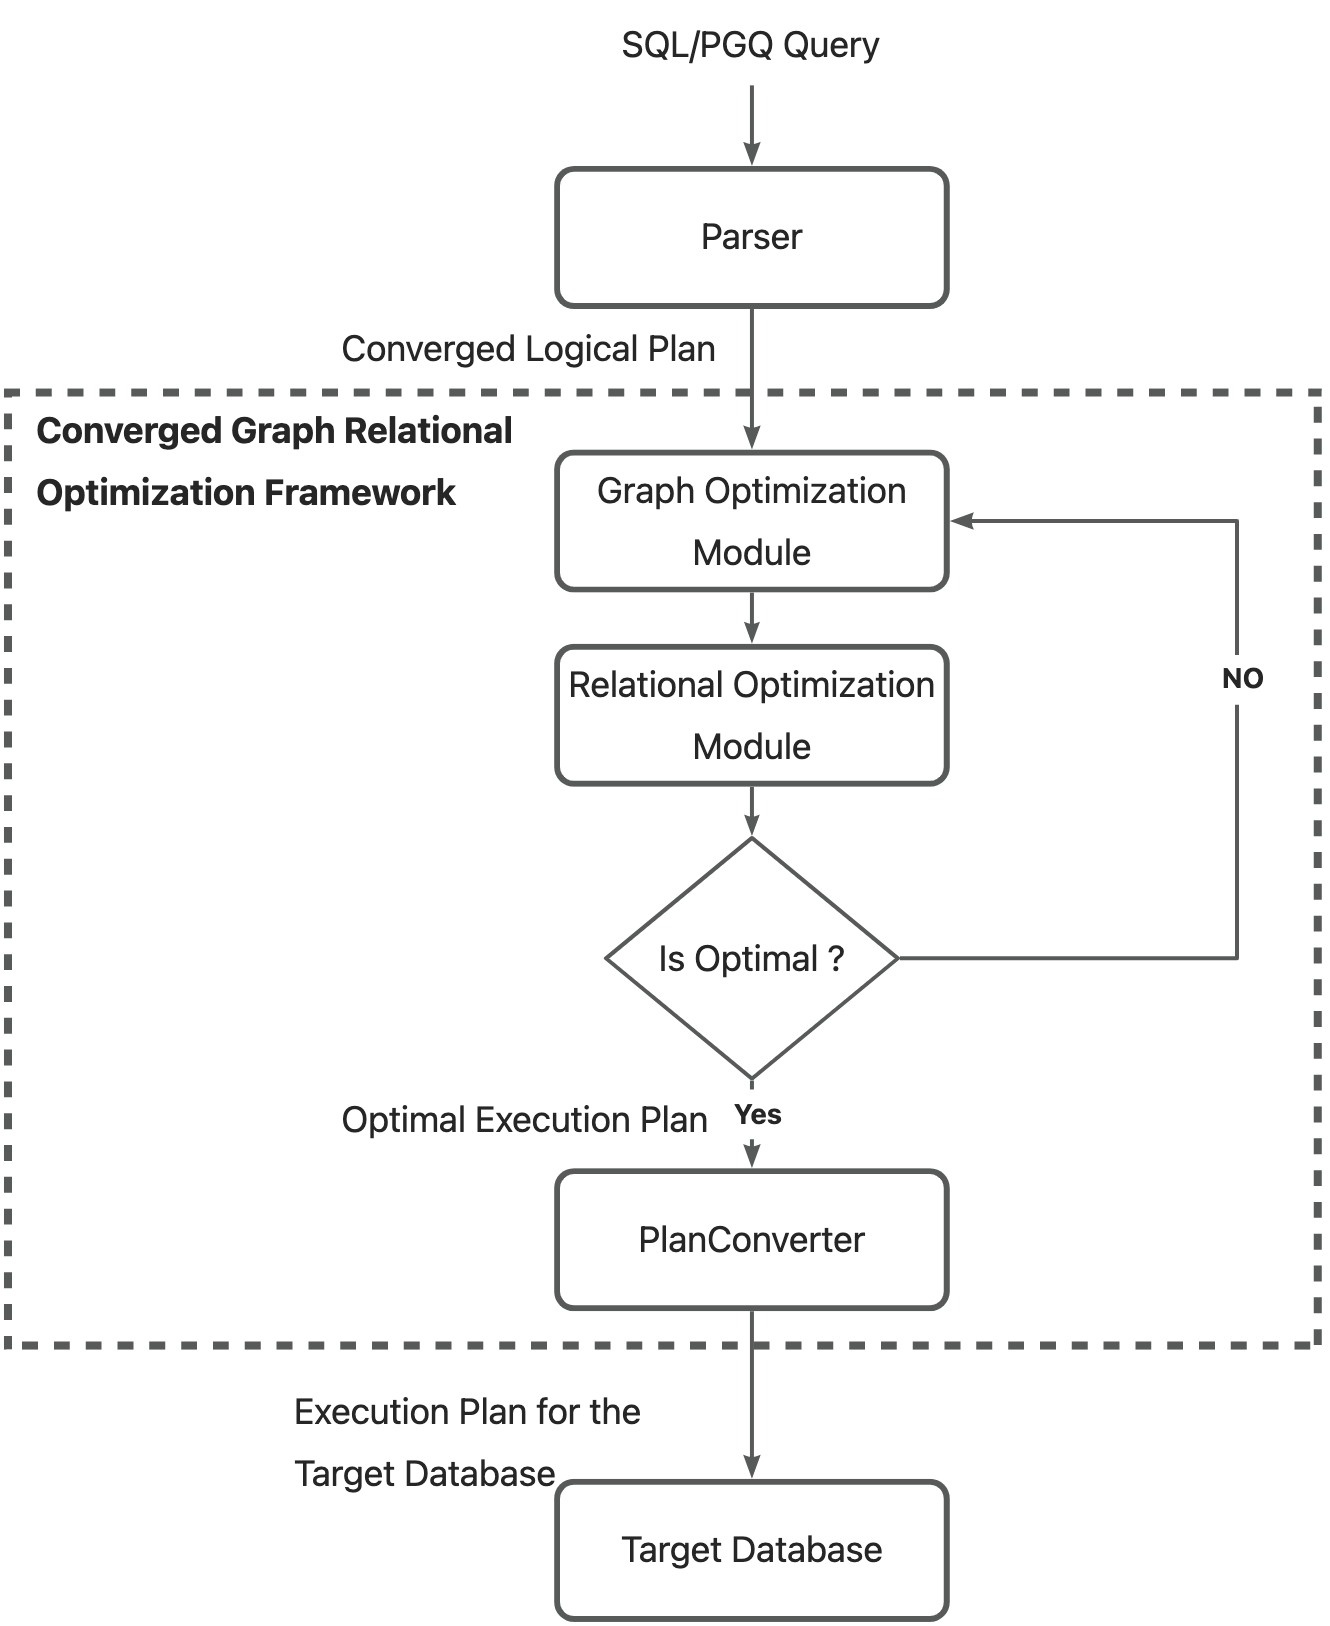
\includegraphics[width=.8\linewidth]{./figures/workflow.png}
    \caption{Workflow of the Converged Graph Relational Optimization Framework.}
    \label{fig:workflow}
\end{figure}

\begin{figure}
    \centering
    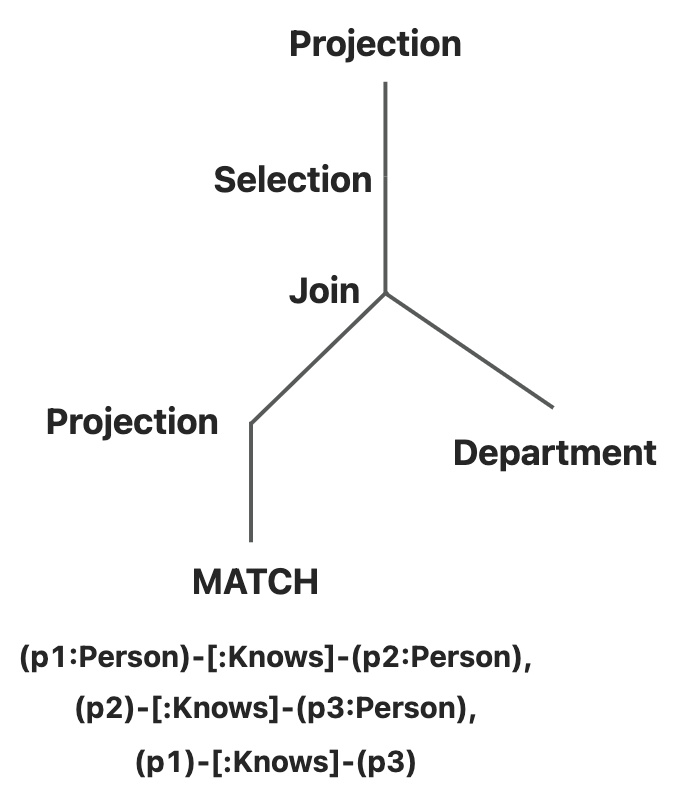
\includegraphics[width=.6\linewidth]{./figures/example_tree.png}
    \caption{The operator tree of SPJM query in Example \ref{example:framework}.}
    \label{fig:example-operator-tree}
\end{figure}

\begin{figure*}
    \centering
    \begin{subfigure}[b]{0.4\linewidth}
        \centering
        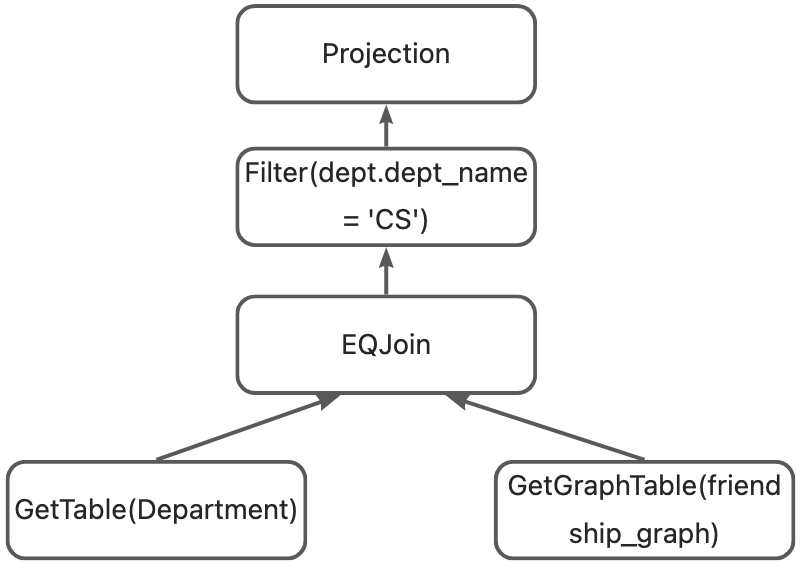
\includegraphics[width=\linewidth]{./figures/converged-logical-plan-relational.png}
        \caption{Outer query plan.}
        \label{fig:converged-logical-plan-relational}
    \end{subfigure}
    \begin{subfigure}[b]{0.4\linewidth}
        \centering
        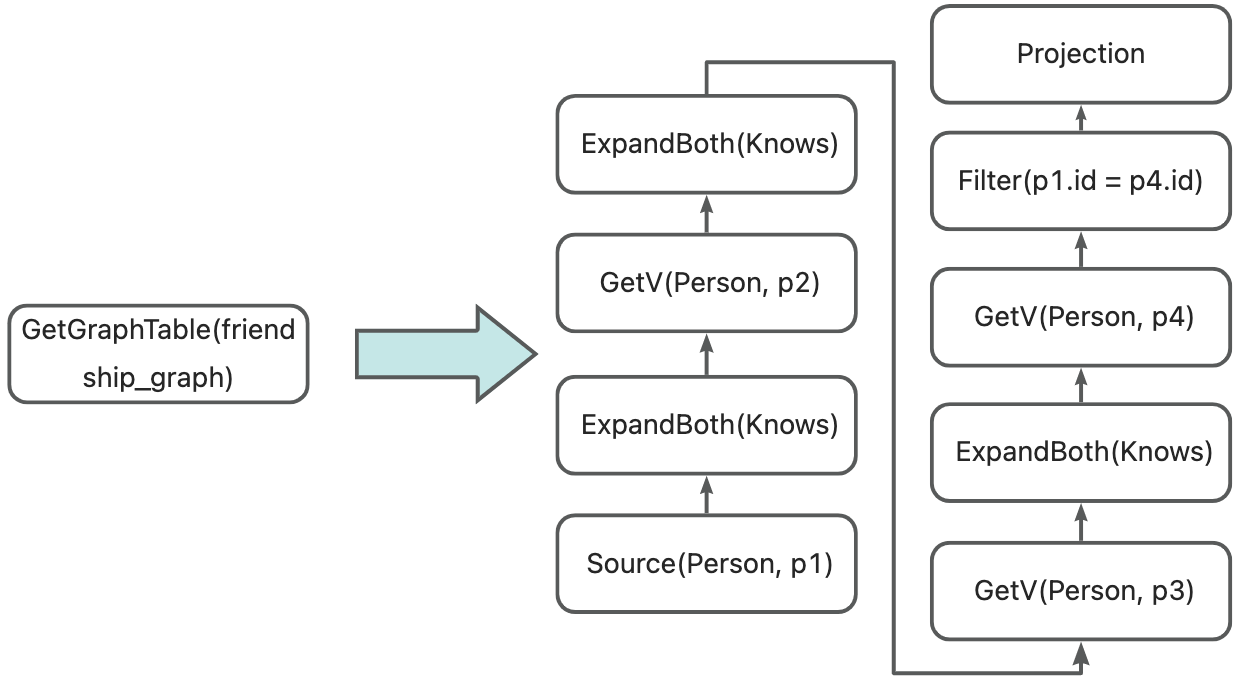
\includegraphics[width=\linewidth]{./figures/converged-logical-plan-graph.png}
        \caption{Match scanning plan.}
        \label{fig:converged-logical-plan-graph}
    \end{subfigure}
    \begin{subfigure}[b]{0.4\linewidth}
        \centering
        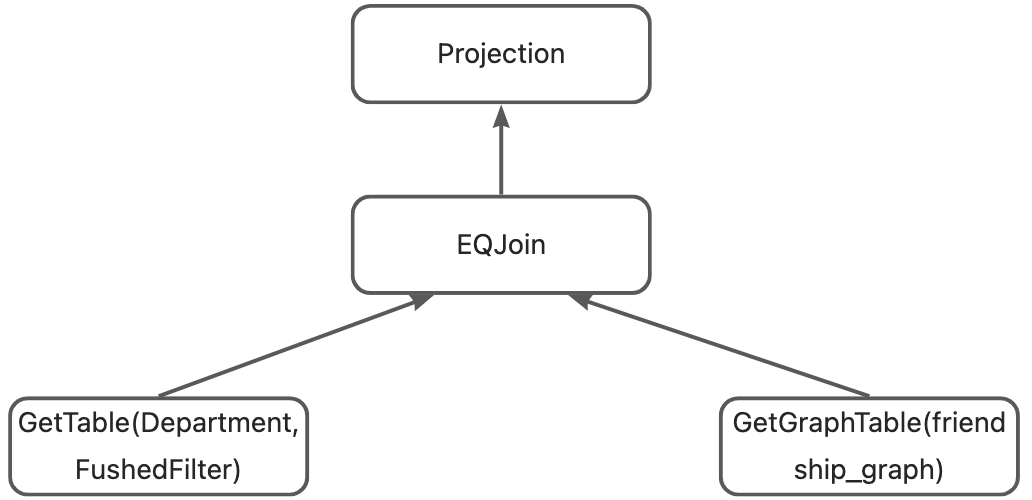
\includegraphics[width=\linewidth]{./figures/converged-logical-plan-relational-optimized.png}
        \caption{Outer query plan after Optimization.}
        \label{fig:relational-plan-optimized}
    \end{subfigure}
    \begin{subfigure}[b]{0.4\linewidth}
        \centering
        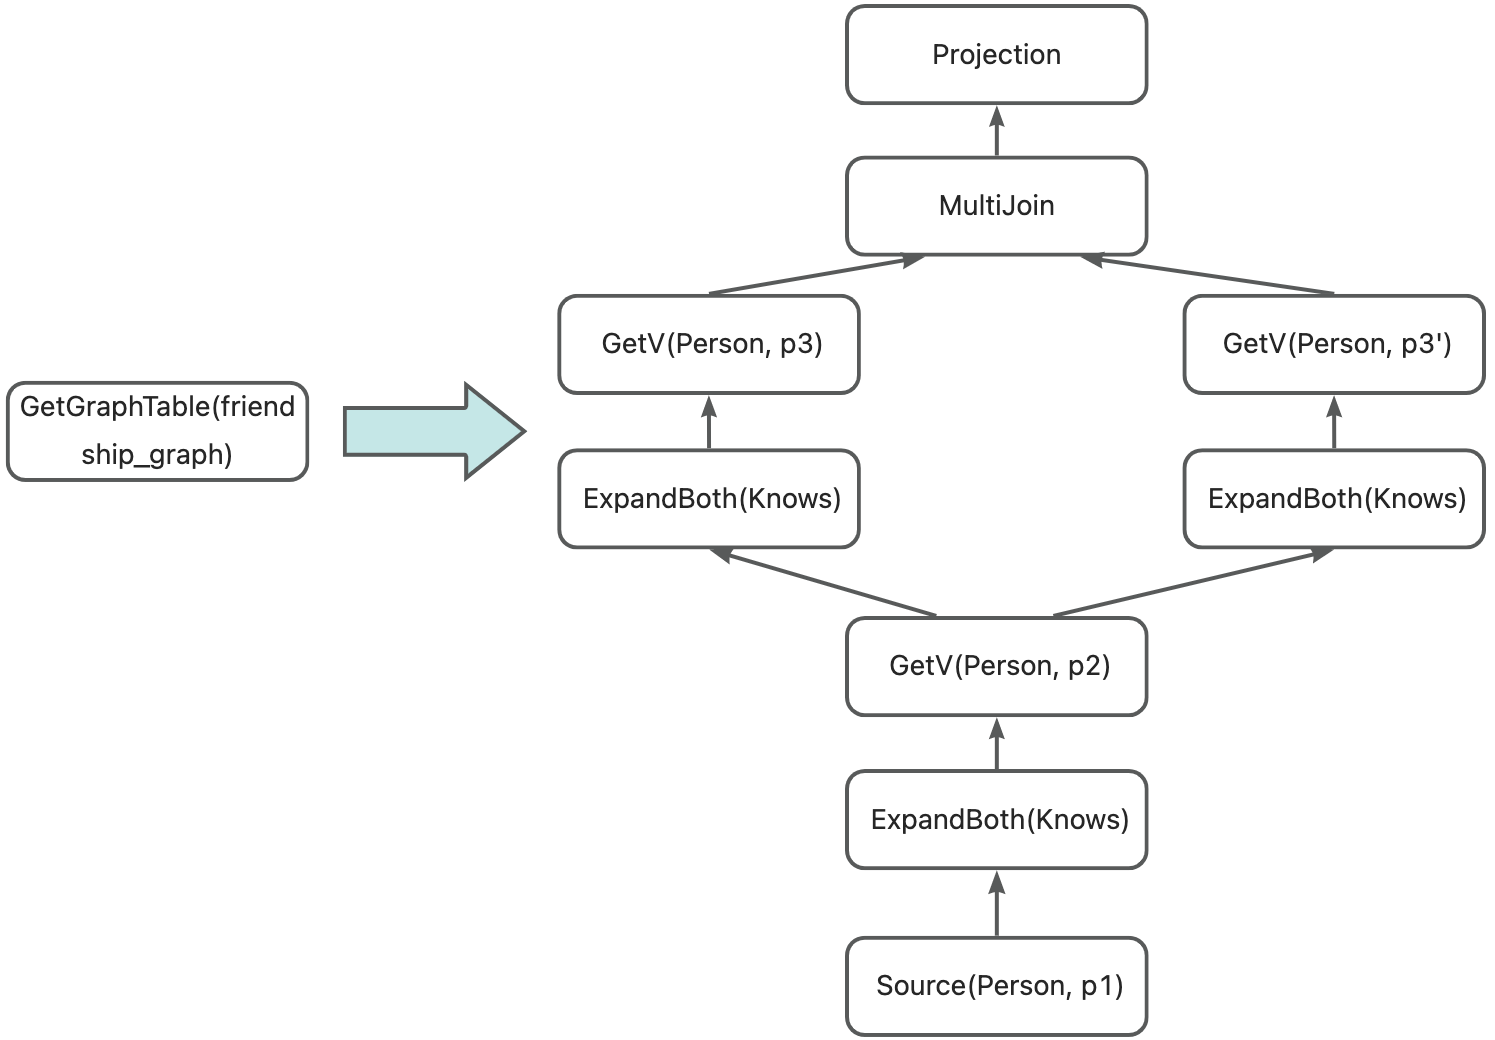
\includegraphics[width=\linewidth]{./figures/converged-logical-plan-graph-optimized.png}
        \caption{Match scanning plan after Optimization.}
        \label{fig:graph-plan-optimized}
    \end{subfigure}
    \begin{subfigure}[b]{0.5\linewidth}
        \centering
        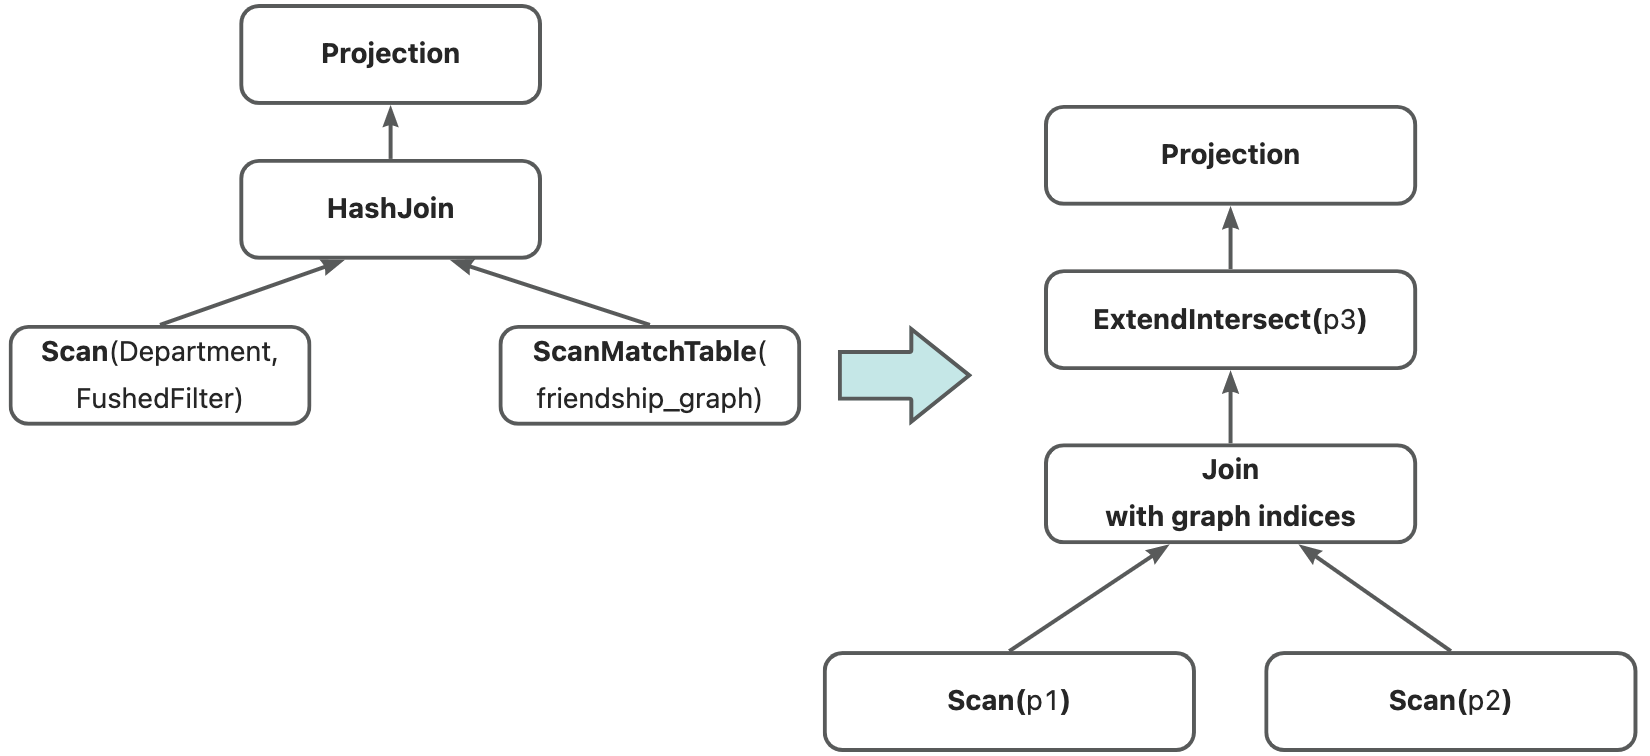
\includegraphics[width=\linewidth]{./figures/converged-physical-plan.png}
        \caption{Obtained Optimal Physical Plan.}
        \label{fig:physical-plan-optimized}
    \end{subfigure}
    \caption{An example of query optimization.}
    \label{fig:query-grtree-example}
\end{figure*}



The above process of query processing is illustrated with the following example.

\begin{example}
    \label{example:framework}
    Given a relational database with tables as follows,
    \begin{equation*}
        \begin{split}
            & \textit{Person = (\underline{id}, name, dept\_id)} \\
            & \textit{Knows = (\underline{id1}, \underline{id2})} \\
            & \textit{Department = (\underline{dept\_id}, dept\_name)}, \\
        \end{split}
    \end{equation*}
    suppose we are going to find three persons satisfying:
    (1) These three persons know each other;
    (2) At least two of them are from the department of computer science.
    The SPJM query can be illustrated as shown in Fig.~\ref{fig:example-operator-tree}.

    In relational matching algebra, the SPJM query can be expressed as follows:
    Firstly, to obtain the triangles, the pattern $\mathcal{P}_{\triangle}$ is
    \begin{lstlisting}
        (p1:Person)-[:Knows]-(p2:Person),
        (p2)-[:Knows]-(p3:Person),
        (p1)-[:Knows]-(p3)
    \end{lstlisting}
    Then, to get the relational table that records the three person and their departments, the algebra expression is
    \begin{equation*}
        \begin{split}
            \widehat{R}_{graph} = & \pi_{p1.name\rightarrow pn1, p1.dept\_id \rightarrow dept1,p2.name\rightarrow pn2, p2.dept\_id \rightarrow dept2,} \\
            & _{p3.name\rightarrow pn3, p3.dept\_id \rightarrow dept3}(\mathcal{M}(GR, \mathcal{P}_{\triangle})),
        \end{split}
    \end{equation*}
    where $GR$ is a graph relation with only one tuple, and each attribute of the tuple is a vertex or an edge.
    The vertices correspond to rows in table Person and edges correspond to rows in table Knows.

    Finally, to obtain the triangles of persons with at least two persons from the department of computer science, the algebra expression is
    \begin{equation*}
        \begin{split}
        \pi_{pn1, pn2, pn3}
        (& \sigma_{dept.dept\_name = \text{`Computer Science'}}( \\
        & dept \Join_{dept1=dept.dept\_id \land dept2=dept.dept\_id} \widehat{R}_{graph})).
        \end{split}
    \end{equation*}

    Based on the above algebra expressions, the match scanning plan is shown in Fig.~\ref{fig:converged-logical-plan-graph} and the outer query plan is shown in Fig.~\ref{fig:converged-logical-plan-relational}.

    Then, optimization modules in the optimization layer are applied to optimize the plans.
    The optimized plans are shown in Fig.~\ref{fig:relational-plan-optimized} and Fig.~\ref{fig:graph-plan-optimized}.
    Moreover, the finally obtained optimal physical plan is shown in Fig.~\ref{fig:physical-plan-optimized}.
\end{example}
}

%\section{Optimizations}
\label{sec:optimizations}

The relational optimization module and graph optimization module optimize he relational plan and graph plans, respectively.
In this subsection, we present the details of the optimization strategies utilized in these two modules. 

\subsection{Optimization Strategies in Relational Optimization Module}

Like most relational optimizers, the relational optimization module applies both Rule-based Optimization (abbr.~RBO) and Cost-based Optimization (abbr.~CBO) strategies on relational subplans for a better physical plan.
In detail, in terms of RBO, commonly used optimizations such as filter pushdown, join order optimization, and removal of unused columns are employed in the converged optimizer.
In terms of CBO, the costs of plans are estimated based on the low-order statistics such as the cardinalities of tables and query conditions.

Besides, since a new operator, i.e., GraphTableScan, is added for relational optimizer, it is possible to perform some optimization across the relational and graph subplans.

\filterrule. 
Inspired by FilterPushdownRule in relational optimizer, which can push down the predicates to the Scan operator to filter out invalid elements earlier, we propose \filterrule.
As the ScanGraphTable operator is a special kind of Scan operator which acts like scanning a table obtained by a graph subplan, it is reasonable to integrate the filtering criteria into the ScanGraphTable operator.
Specifically, the \filterrule seeks to push predicates on properties of graph elements from the relational subplan to graph subplans, so that invalid graph elements can be dropped earlier.
An example of applying \filterrule is given in Example \ref{example:push_down}.

Specifically, \filterrule can embed filter conditions into basic graph operators like \scan~, \expandedge~, or \getvertex~ to further push down filter conditions in graph queries. 
This integration allows the direct exclusion of vertices and edges not satisfying the filter conditions, thus drastically cutting down the volume of intermediary outcomes.

Formally, the equation rule w.r.t.~\filterrule is as follows:
\begin{equation}
    \begin{split}
    & \sigma_{\theta}\pi_{v.a_1, \cdots, v.a_k}(lr~\alpha_{(u)}^{(v)}[e]~er) \\
    & \hspace*{2em} \equiv \pi_{v.a_1, \cdots, v.a_k}(lr~\sigma_{\theta}(\alpha_{(u)}^{(v:vLabel)}[e]~er)), \\
    \end{split}
\end{equation}
where $lr$ and $er$ are graph relational algebra expressions, $\alpha \in \{\uparrow, \downarrow, \updownarrow\}$, and vLabel is specified if the label of $v$ is specified in $\theta$.


\intersectrule. 
Please note that the intersection operator is not defined in graph queries, but it can be expressed with expand operators.
Given a SQL/PGQ query, if the two subqueries that intersect are both graph queries, then the paths in these two graph queries can be combined with expand operators to generate new paths.
That is, two graph queries combined with an intersection operator are converted to a new graph query.
By leveraging graph indices, it can be more efficient to obtain the intersection results w.r.t.~the new graph query.
To some extent, one of the graph queries can be considered as the predicates, and then \intersectrule is somehow pushing down predicates to the other graph query.
The rule is as follows.
\begin{equation}
    \begin{split}
        & \pi_{v.a_1, \cdots, v.a_k}(el~\alpha_{(u)}^{(v:vlabel)}[e]~er) \\
        & \hspace*{2em} \equiv \pi_{v.a_1, \cdots, v.a_k}(el) \cap \pi_{v.a_1, \cdots, v.a_k}(\alpha_{(u)}^{(v:vlabel)}[e]~er),
    \end{split}
\end{equation}
where $el$ and $er$ are graph relational algebra expressions, $\alpha \in \{\uparrow, \downarrow, \updownarrow\}$.

\begin{example}
    Suppose we are going to find persons that know both Alice and Bob, the corresponding relational query is as follows:
    \begin{lstlisting}
        (
            SELECT p2.name
            FROM Person p1, Knows k1, Person p2
            WHERE k1.sid = p1.id
                AND k1.tid = p2.id
                AND p1.name = 'Alice'
        )
        INTERSECT
        (
            SELECT p2.name
            FROM Person p2, Knows k2, Person p3;
            WHERE k2.sid = p2.id
                AND k2.tid = p3.id
                AND p3.name = 'Bob';
        )
    \end{lstlisting}
    Then, based on the \intersectrule, the query can be transformed to the corresponding graph query as follow:
    \begin{lstlisting}
        SELECT name 
        FROM GRAPH_TABLE (know_graph
            MATCH (p1:Person {name: 'Alice'})-[k1:Knows]->(p2:Person)<-[k2:Knows]-(p3:Person {name: 'Bob'})
            COLUMNS (p2.name as name);
        );
    \end{lstlisting}
\end{example}



\subsection{Optimization Strategies in Graph Optimization Module}

In the graph optimization module, we formulate a specific rule set to capitalize on optimization potential among graph operators. 
Both RBO and CBO strategies are included in the rule set.

In terms of RBO strategies, two frequently utilized key rules, i.e., \trimrule and \fusionrule, are presented in this subsection.

\trimrule. 
The \trimrule~ is a well-established relational optimization strategy that removes superfluous data at intermediary stages of query processing. 
Two particular instances where trimming helps include: 
Firstly, \trimrule~ can eliminate intermediate results with aliases that are not required and reduce computations.
Secondly, it involves discarding unneeded vertex and edge properties when retrieving from the data graph. 
This is accomplished by specifying essential properties in the graph operators’ \code{COLUMNS} field.
Formally, an example of applying \trimrule is as follows:
\begin{equation}
    \mathcal{S}_g \Rightarrow \pi_{u.a_1, \cdots, u.a_k}\mathcal{S} _g 
\end{equation}
where $\mathcal{P}_g$ is a graph relational algebra expression corresponding to a graph subplan, and $u.a_1, \cdots, u.a_k$ are necessary properties.


\fusionrule. 
The \fusionrule~ is a graph-centric rule. 
Commonly in graph queries, a sequence of \expandedge~ followed by \getvertex~ indicates a search for neighboring vertices. 
The \fusionrule~ consolidates these operators into one integrated \expandvertex~ to boost efficiency. 
Nonetheless, whether \expandedge~ and \getvertex~ can be merged is context-dependent. 
For example, if some properties of the edges are needed, fusion might not be feasible.
This rule evaluates such factors to ensure query optimization without compromising result integrity.
%Formally, an example of applying \fusionrule is as follows:
%\begin{equation}
%    \begin{split}
%    &  \\
%    & \hspace*{2em} \Rightarrow \pi_{u.a_1, \cdots, u.a_k}\updownarrow_{(u)}^{(v:vLabel)}[:eLabel](\sigma_{d(u)}\bigcirc_{(u:uLabel)}), \\
%    \end{split}
%\end{equation}
%where $d(u)$ is a filtering constraint on vertex $u$.


\expandintersectrule.
The \expandintersectrule replaces expand operators that expands to the same vertices with a new operator, i.e., the extend-intersect operator, to reduce the overhead of extending a partial pattern to a new vertex.
This new operator is a new kind of join, and is defined as follows:

\begin{equation}
    \begin{split}
        & R \Diamond^{l_1^{1}|\cdots|l_1^{k_1}, \cdots, l_n^{1}|\cdots|l_n^{k_n}}_{v_1, \cdots, v_n} P = \\ 
        & \hspace{1em} \pi_{\mathcal{R} \cup \mathcal{E} \cup \mathcal{P}}(\sigma_{\lambda(e) = (R.v_1, P.v) \land (\text{Type}(e) = l_1^1 \lor \cdots \lor \text{Type}(e) = l_1^{k_1})}(R \times E \times P)) \\
        & \hspace{1em} \Join \cdots \\
        & \hspace{1em} \Join \pi_{\mathcal{R} \cup \mathcal{E} \cup \mathcal{P}}(\sigma_{\lambda(e) = (R.v_n, P.v) \land (\text{Type}(e) = l_n^1 \lor \cdots \lor \text{Type}(e) = l_n^{k_n})}(R \times E \times P)),
    \end{split}
\end{equation}
where $P$ is a graph relation and each row of $P$ is a vertex,
$E$ is a graph relation containing all the edges in the graph, 
$\mathcal{R}$, $\mathcal{E}$, and $\mathcal{P}$ are the schemas of $R$, $E$, and $P$, respectively,
and $v_1, \cdots, v_n$ are the vertices in $R$ that should connect to vertices in $P$.
The type of the edge between $v_j$ and $p.v$ needs to be one of $\{l_j^1, \cdots l_j^{k_j}\}$.

Given a openCypher query as follows:
\begin{lstlisting}
    MATCH (p1:Person)-[:Likes]->(m:Message),
        (p1)-[:Knows]-(p2:Person)-[:Likes]->(m:Message)
    RETURN p1.name;
\end{lstlisting}
With $\updownarrow^{(p2\text{:Person})}_{(p1)}[\text{:Knows}]\bigcirc_{(p1\text{:Person})}$, the partial results w.r.t.~$(p1)-[\text{:Knows}]-(p2)$ are obtained (denoted by $r$). 
$r$ should be extended to the message $m$ from $p1$ and $p2$ respectively, and then intersection on $m$ is applied.
Therefore, the extend-intersect operator is used, and the query can be compiled to
\begin{equation}
    \left(\updownarrow^{(p2\text{:Person})}_{(p1)}[\text{:Knows}]\bigcirc_{(p1\text{:Person})}\right) \hspace{0.2em} \Diamond_{p1, p2}^{\text{Likes, Likes}} \hspace{0.2em} \bigcirc_{m\text{:Message}}.
\end{equation}

Please note that the extend-intersect operator is friendly to vectorized query processing.
Compared with natural joins, in the process of extend-intersection, fewer vectors are flattened and the time cost is significantly reduced.


In terms of CBO, drawing from insignts gained in the prior research, we implement effective pattern matching by incorporating hybrid pattern join strategies and leveraging high-order statistics, which provide a more granular understanding of the data through the frequency of smaller patterns.
Moreover, the prior research has some drawbacks, including using a bottom-up search framework that potentially missed early pruning opportunities and having a narrow focus on basic patterns without accommodating union patterns scenarios.
Therefore, we also introduce a novel top-down search framework, inclusive of branch-and-bound pruning strategies, and devise specific cardinality estimation methods for union patterns. 
Besides, in this implementation, we use a rule for pattern transformation to ensure all modifications maintain the original results’ integrity.
Furthermore, for pattern matching, we consider binary join and extend-intersect operators. 
The binary join applies a hash-join on two pattern mappings to produce a larger pattern's results.
The extend-intersect operator optimizes the process when only one vertex is added to the existing pattern. 
This expansion can vary from a simple addition of a single new edge to more complex scenarios involving multiple edges, implemented through optimal joins.

Regarding cost and cardinality estimation, we adopt a cost model that considers both the communication costs of intermediate result transfer in distributed environments and the computational costs of physical plan operators. 
Specifically, costs for the binary join and extend-intersect operators in graphs are defined. 
Additionally, we estimate the operator cost using an expand ratio that reflects the change in pattern occurrences when edges are expanded.

%\section{Superiority of Relgo in Optimization}
\label{sec:theoretical-analysis}

In this section, we prove that graph optimizers have better performance than relational optimizers on graph query optimization.
It confirms that translating graph queries into relational queries to be optimized with relational optimizers is not a good choice.

As one of the most widely adopted optimizers for relational databases, we use Calcite \cite{calcite,columbia} as a representative of relational optimizers and analyze its efficiency.
For relgo, Calcite is also used as the relational optimization module.
Meanwhile, GLogue \cite{GLogS} is applied as the graph optimization module.

For simplicity, we focus on the problem of join order optimization in this section, and a simple case is first considered.
That is, all the tables in the query represent vertices or edges.
The tables that can represent vertices or edges are called graph tables, and the graph formulated by these graph tables are called a query graph.
Then, assuming that there are $n + m$ graph tables joined together, with $n$ tables representing vertices and $m$ tables representing edges.
Suppose that there are $t$ implementation methods for join.
Noramlly, various kinds of joins are supported in relational databases, e.g., hash join, merge join, and index join.
Consequently, it is supposed that $t \geq 2$.
The complexities of optimizing the join order with Calcite and relgo are analyzed respectively as follows.
For simplicity, the time complexities are estimated with the number of physical plans generated by the optimizers.


\begin{theorem}
    \label{theorem:complexity-of-calcite}
    The time complexity of join order optimization with Calcite is at least $O(4^{m+n-1})$.
\end{theorem}
\begin{proof}
    The $n + m$ tables joined together can form a graph, where the tables represent vertices in the graph, and if there is a join condition w.r.t.~two tables, there is an edge between these two tables.
    Then, the complexity of join order optimization with Calcite can be estimated as the number of possible physical plans that can be generated.
    
    To avoid cross product, everytime two tables are joined together, there should be join conditions w.r.t.~them.
    Therefore, the join order can be represented as a spanning tree in the graph.
    By computing the number of physical plans can be generated according to each spanning tree, the total number of physical plans can be obtained.
    %%%
    %However, same phyical plans may be obtained according to different spanning trees.
    %For example, suppose a graph is a rectangle with four vertices and four edges.
    %It may be constructed for a query like:
    %\begin{equation*}
    %    \begin{split}
    %        \text{SELECT}\hspace{.5em} ... & \hspace{.5em}\text{FROM}\hspace{.5em} A, B, C, D \hspace{.5em}\text{WHERE}\hspace{.5em} A.a1 = B.b1 \\ 
    %        & \hspace{.5em}\text{AND}\hspace{.5em} B.b2 = C.c1 \hspace{.5em}\text{AND}\hspace{.5em} C.c2 = D.d1 \hspace{.5em}\text{AND}\hspace{.5em} D.d2 = A.a2. 
    %    \end{split}
    %\end{equation*}
    %Then, the spanning tree with edges \{AB, BC, CD\} and the one with edges \{AB, BC, AD\} can generate the same physical plans.
    %Consequently, the summation of the number of physical plans corresponding to all the spanning trees is larger than the actual number of physical plans.
    In this proof, we compute the number of physical plans for one spanning tree, and this number is the lower bound of the number of physical plans that can be generated.

    We start with a spanning tree with $k$ edges ($k \geq 1$), which has only one leaf node (i.e., it is a path).
    Then, the number of logical plans corresponding to the spanning tree is
    \begin{equation*}
        \begin{split}
            c_l(k) & = 2 * (c(0)c(k-1) + c(1)c(k-2) + \cdots + c(k-1)c(0)) \\
            & = 2\Sigma_{i=0}^{i=k-1}c(i)c(k-1-i), \\
            & \text{where } c_l(0) = 1.
        \end{split}
    \end{equation*}
    With the generating function, it is obtained that 
    \begin{equation*}
        \begin{split}
            c_l(k) & = \frac{2^k}{k+1}C(2k, k) \geq \frac{2^k}{k+1}\frac{2k \times \cdots \times (k+1)}{k \times \cdots \times 1} \\
            & \geq \frac{2^k}{k+1}2^{k-1}(k+1) = \frac{4^k}{2}
        \end{split}
    \end{equation*}
    %Since $k$ is the number of edges, and $k = m + n - 1$ in the spanning tree.
    %Thus, the number of logical plans w.r.t.~a spanning tree is 
    %\begin{equation*}
    %    \frac{2^{m+n-1}}{m+n}C(2m+2n-2, m+n-1) \geq \frac{4^{m+n-1}}{m+n}.
    %\end{equation*}

    For any spanning tree $T$ with $k = m + n - 1$ edges, denote the longest path in the tree by $p_1$, and its length is $P_1 = |p_1|$.
    By removing the path (i.e., edges in $p_1$) from $T$, we can obtain a new subgraph $T_1$.
    Similarly, the longest path in $T_1$ that intersects with the already removed paths (i.e., $p_1$) is found and denoted by $p_2$, with $P_2 = |p_2|$.
    After that, $p_2$ is removed from $T_1$ and subgraph $T_2$ is obtained.
    For $p_1$ and $p_2$, since they are both paths, the numbers of logical plans corresponding to them are $c_l(P_1)$ and $c_l(P_2)$, respectively.
    Without loss of generality, suppose $p_1$ and $p_2$ intersects at vertex $v_i$, and then, $v_i$ appears in each logical plan corresponding to $p_1$.
    Then, by replacing $v_i$ with the plans corresponding to $p_2$, respectively, $c(p_1 \cup p_2) \geq c_l(P_1)c_l(P_2)$ is obtained, where $c(t)$ is the number of logical plans corresponding to tree $t$ and $c(t) = c_l(k)$ when $t$ is a path with $k$ edges.

    As $T$ is a tree, by repeatedly finding and removing the paths as above, all the edges in $T$ are finally removed.
    Let the number of paths removed be $s$, we have 
    \begin{equation*}
        \begin{split}
            c(T) & = c(p_1 \cup \cdots \cup p_s) \geq c_l(P_1) \cdots c_l(P_s) \\
            & \geq \frac{4^{P_1 + \cdots + P_s}}{2^s} = \frac{4^{m + n - 1}}{2^s} \geq 2^{m+n-1}.
        \end{split}
    \end{equation*}
    
    %Thus, the number of logical plans w.r.t.~a spanning tree is 
    %\begin{equation*}ƒ
    %    \frac{2^{m+n-1}}{m+n}C(2m+2n-2, m+n-1) \geq \frac{4^{m+n-1}}{m+n}.
    %\end{equation*}
    

    Thus, the number of physical plans is at least $2^{m+n-1}t^{m+n-1} \geq 4^{m+n-1}$, so is the complexity of join order optimization with Calcite.
   
    In conclusion, Theorem \ref{theorem:complexity-of-calcite} is correct.
\end{proof}

\begin{lemma}
    \label{lemma:upper-bound-of-calcite}
    Given $z$ tables, the time complexity of join order optimization with Calcite has an upper bound of $O(\frac{(2z-2)!}{(z-1)!}t^{z-1})$.
\end{lemma}
\begin{proof}
    The upper bound of the time complexity of join order optimization is achieved when there is a condition between any two of the $z$ tables.
    Because at that time, the tables can be joined in any order.

    Since each join order corresponds to a full binary tree with $2z-1$ nodes, the problem is to count the number of possible full binary trees.
    Similar to Catalan number, the number of full binary trees is $O(C(2z-2, z-1) - C(2z-2, z))$.
    For each full binary tree, there are $z!$ ways to set the leaf nodes. 
    Then, the number of generated physical plans is $O(\frac{(2z-2)!}{(z-1)!}t^{z-1})$.
\end{proof}


\begin{theorem}
    \label{theorem:complexity-of-glogue}
    The time complexity of join order optimization with relgo is smaller than $3^n$ if all the tables participant in join are graph tables.
\end{theorem}
\begin{proof}
    Since the $n + m$ tables are graph tables, relgo optimizes the join order with the graph optimization module, i.e., GLogue.

    As GLogue ensures worst-case optimality and the considered patterns are all induced subgraphs, the time complexity of join order optimization with GLogue is not related to the number of edges (i.e., $m$).
    Since the join order optimization problem is reduced to a variant of the shortest path problem, the time complexity is $O(\mathcal{E})$, where $\mathcal{E}$ is the number of edges in GLogue.
    In detail, 
    \begin{equation*}
        \begin{split}
            %O(\mathcal{E}) & = C(n, n-1)*(2^{n-1}-1) + C(n, n-2) * (2^{n-2}- 1) \\
            %& + \cdots + C(n, 1) * (2^1 - 1) \\
            O(\mathcal{E}) & = \Sigma_{i=1}^{i=n-1}C(n, i)(2^i - 1) = 3^n - 2^{n+1} +1 < 3^n.
        \end{split}
    \end{equation*}
    
    In conclusion, Theorem \ref{theorem:complexity-of-glogue} is correct.

\end{proof}

Based on the complexity analysis in Theorem \ref{theorem:complexity-of-calcite} and Theorem \ref{theorem:complexity-of-glogue}, it is found that when the tables represent vertices and edges, 
\begin{equation*}
    \begin{split}
        \frac{\text{Time Complexity of Calcite}}{\text{Time Complexity of relgo}} & > O(\frac{4^{m+n-1}}{3^n}) = O(4^{m-1}(\frac{4}{3})^n).
    \end{split}
\end{equation*}
Therefore, it suggests that relgo is exponentially faster than Calcite for graph-like join order optimization.
The results also indicate that integrating graph optimizers into relational optimizers can improve the efficiency of join order optimization significantly.


Then, to be more general, if there are some tables that cannot represent vertices or edges, the order of such tables cannot be optimized only with graph optimizers, and the problem becomes more complicate.
For example, suppose five tables form a clique, and then these tables cannot be vertices or edges in a graph.
According to relgo, the join order of the graph tables are optimized with GLogue.
The plan obtained by GLogue is considered as a table and optimized together with the left tables (which are not graph tables) by Calcite.
Without the loss of generality, the query graph formulated by the graph tables are assumed to be connected.
When the query graph is not connected, only one connected component of the query graph is optimized with GLogue.
The other tables are not considered as graph tables and are optimized with Calcite.
The efficiency of relgo and Calcite are compared with the following lemma and theorem.

%Specifically, according to the dataflow shown in Fig.~\ref{fig:dataflow}, the join order of these left tables are optimzed by relational optimizers such as Calcite.
%Let the number of left tables be $q$, and together with the table obtained by the join of the tables optimized with graph optimizer, Calcite needs to optimize the join order among $q + 1$ tables.

\iffalse
When $q = 0$, all the tables represent vertices or edges, and the time complexity of relgo is exponentially smaller than that of Calcite as analyzed as above.

When $q = 1$, only one table (saying $T_1$) does not represent a vertex or an edge, and Calcite optimizes the join between two tables.
One of these two tables is $T_1$, and the other is the table obtained by the join of the tables optimized with the graph optimizer.
Then, we have
\begin{equation*}
    \begin{split}
        \frac{\text{Time Complexity of Calcite}}{\text{Time Complexity of relgo}} > \hspace{-12em} & \\
        & \frac{\frac{2^{m+n-1}}{m+n}C(2m+2n-2, m+n-1)t^{m + n - 1}}{3^{\hat{n}} + \frac{(2s)!}{(s)!}t^{s}} \\
        & = \frac{\frac{2^{m+n-1}}{m+n}C(2m+2n-2, m+n-1)t^{m + n - 1}}{3^{\hat{n}} + 2} >> 1,
    \end{split}
\end{equation*}
where $\hat{n}$ is the number of tables representing vertices.
It indicates the superiority of the converged JOPT.

When $s = m + n - 1$ or $p = m + n$, at most one table can represent vertices or edges, and the converged JOPT degenerates to Calcite, and has the same efficiency as it.
A typical example is when there is a condition between any two of these $m + n$ tables.

The results show that the converged JOPT is always superior to relational JOPTs.
To be more specific, we prove the superiority of the converged JOPT more theoretically.
\fi

\begin{lemma}
    \label{lemma:join-spliter}
    Let $\text{JN}_c(V_s)$ represent the number of possible physical plans of joining tables in table set $V_s$ with Calcite.
    Suppose $n$ tables (denoted as table set $V$) are joined, and $V = (V_1 - u) \cup V_2$, $V_1 \cap V_2 = \emptyset$.
    Specifically, $u \in V_1$ is a table representing the results of joining the tables in $V_2$.
    For each table $t_2 \in V_2$, if there is a join condition between $t_2$ and a table $v$ in $V_1$, the same join condition exists between $u$ and $v$.
    Then, we have $\text{JN}_c(V) \geq \text{JN}_c(V_1) * \text{JN}_c(V_2)$.
\end{lemma}
\begin{proof}
    For a physical plan generated by joining tables in $V_1$ (denoted as $p_1$) and a plan generated by joining tables in $V_2$ (denoted as $p_2$), by replacing $u$ in $p_1$ with $p_2$, we can generate a physical plan of joining tables in in $V$.
    Besides, since the tables in $p_1$ cannot be interchanged with tables in $p_2$, more physical plans can be generated by joining tables in $V$.
    In conclusion, we have $\text{JN}_c(V) \geq \text{JN}_c(V_1) * \text{JN}_c(V_2)$.
\end{proof}

\begin{theorem}
    \label{theorem:complexity-of-converged-jopt}
    The time complexity of join order optimization with relgo is always smaller than that with Calcite.
\end{theorem}
\begin{proof}
    Denote the set of graph tables by $R$, denote the set of other tables by $S$, and denote the table obtained by joining the tables in $R$ by $T_r$.
    Then, we have $S_r = S \cup T_r$.
    Moreover, let $s = |S|$ and $r = |R|$ represent the size of table sets $S$ and $R$, respectively, and let $r_v$ be the number of tables in $R$ representing vertices.
    Denote the number of possible physical plans of joining tables in $R$ with GLogue by $\text{JN}_g(R)$.
    
    Specifically, according to Theorem \ref{theorem:complexity-of-calcite} and Theorem \ref{theorem:complexity-of-glogue}, we have $4^{r - r_v -1}(\frac{4}{3})^{r_v}\text{JN}_g(R) < \text{JN}_c(R)$.
    % $\text{JN}_g(R) < 3^{r_v} \leq 4^{r-1} \leq \text{JN}_c(R)$.
    Note that $T_r$ corresponds to $u$ in Lemma \ref{lemma:join-spliter}.
    Based on Lemma \ref{lemma:join-spliter}, we have $\text{JN}_c(S \cup R) \geq \text{JN}_c(S_r) * \text{JN}_c(R) \geq 4^{r - r_v -1}(\frac{4}{3})^{r_v} * \text{JN}_c(S_r) * \text{JN}_g(R)$.
    In conclusion, Theorem \ref{theorem:complexity-of-converged-jopt} is correct, and relgo always has exponentially smaller time complexity than Calcite.
\end{proof}

There are mainly three reasons contributing to the efficient performance of the relgo:
(1) Different implementations of the join operators are not considered in relgo, because the neighbors of vertices can be efficiently accessed with the graph indices.
(2) In relgo, only the number of vertices influence the complexity of join order optimization, while the complexity is determined by both the numbers of vertices and edges in Calcite.
(3) relgo can take isomorphism into consideration in optimization and further reduce the search space, while Calcite does not consider optimization related to isomorphism.

\begin{table}[ht]
    \centering
    \begin{tabular}{c|c|c|c|c|c}
    \hline
    Dataset & \#$R_v$ & \#$R_e$ & Avg. \#$R_v$ & Avg. \#$R_e$ & Disk Usage\\
    \hline
    $LDBC10$ & 8 & 12 & 3,748,479 & 7,359,821 & 8.9G \\
    \hline
    $LDBC30$ & 8 & 12 & 11,098,729 & 23,221,036 & 28.0G\\
    \hline
    \revise{$LDBC100$} & 8 & 12 & 35,329,734 & 78,221,268 & 90.0G \\
    \hline
    $IMDB$ & 14 & 7 & 1,030,853 & 8,536,891 & 3.7G \\
    \hline
    \end{tabular}
    \caption{Statistics of the datasets. In detail, \#$R_v$ (resp.~\#$R_e$) is the number of vertex (resp.~edge) relations and Avg.~\#$R_v$ (Avg.~\#$R_e$) is the average number of tuples in a vertex (resp.~edge) relation.}
    \label{table:experiment-datasets}
\end{table}

\section{Evaluation}
\label{sec:evaluation}
% The experimental results are presented and analyzed in this section.
% In detail, experimental settings are introduced in Sec.~\ref{sec:experiment-settings}.
% Sec.~\ref{sec:experiment-e2e}-Sec.~\ref{sec:experiment-case-study} conduct the end-end experiments, test on queries with cycles, perform ablation studies, evaluate the optimization efficiency, test the efficiency of optimziations accross reltaional and graph queries, and evaluate the efficiency of the join order of the plans generated by \name, respectively.


%\enlargethispage{1em}

\subsection{Experimental Settings}
\label{sec:experiment-settings}

\noindent\textbf{Benchmarks.} Our experiments leverage two widely used benchmarks to assess system performance, as follows:
\begin{itemize}
    \item \textbf{LDBC SNB.} We follow the Linked Data Benchmark Council (LDBC) social network benchmark~\cite{ldbc_snb} to test the system. \revise{We use three commonly-adopted datasets with scale factors of 10, 30, and 100, denoted as $LDBC10$, $LDBC30$, and $LDBC100$ respectively, generated by the official LDBC Data Generator}.
    We select 10 queries from the LDBC Interactive workload for evaluation, denoted as $IC[1, \ldots, 9, 11, 12]$, with $10$, $13$, and $14$ excluded since they involve either pre-computation or shortest-path that are not supported.
    To accommodate queries containing variable-length paths~\cite{graindb}, we followed~\cite{graindb} to slightly modify them by separating each query into multiple individual queries with fixed-length paths. Each of these modified queries is denoted with a suffix ``-l'', where $l$ represents the length of the fixed-length path. In addition, we carefully designed two sets of queries for the comprehensiveness of evaluation, including (1) $QR[1\ldots 4]$ to test the effectiveness of heuristic rules \filterrule and \joinfuserule in \name, and (2) $QC[1\ldots 3]$, comprising three typical patterns with cycles including triangle, square, and 4-clique, to assess the efficiency of $\expandintersect$ introduced in \refsec{physical-operators}.
    \item \textbf{JOB.} The Join Order Benchmark (JOB)~\cite{job_snb} on Internet Movie Database (IMDB) is adopted. We select the variants marked with ``a'' of all JOB queries, referred to as $JOB[1\ldots 33]$, without loss of generality. These queries are primarily designed to test join order optimization, with each query containing an average of $8$ joins.
\end{itemize}
The details of the dataset statistics are summarized in Table \ref{table:experiment-datasets}.
We manually implement the queries using SQL/PGQ, which are presented in the artifact~\cite{artifact}.
\revise{In addition, we store the datasets in DuckDB and construct both the EV-index and VE-index on potential edge relations, following the procedures described in GraindB~\cite{graindb}. Specifically, the indices are built on foreign keys and tables that depict many-to-many relationships}.
%In addition, we adhered to the same procedures for data loading and graph index construction as those described in~\cite{graindb}. 
Furthermore, we perform the \rgmapping process in a manner that allows the construction of the same graph index on the LDBC and JOB datasets used in GrainDB's experiments~\cite{graindb}.
%The \rgmapping{s} are defined to ensure the effectiveness of the graph index defined in graindb.


\noindent\textbf{Compared Systems. }
To ensure a fair comparison, \revise{all the following systems except for Kùzu use DuckDB as the underlying relational execution engine. They differ in the adoption of the optimizer.
Kùzu utilizes its own execution engine due to its nature as a graph database management system (GDBMS)}.

\begin{itemize}
\item DuckDB~\cite{duckdb}: This system optimizes queries using the graph-agnostic approach, leveraging DuckDB's built-in optimizer as described in \refsec{relational-only}. It serves as the naive baseline for extending a relational database system to support \spjm.

\item GrainDB~\cite{graindb}: This system uses same optimizer as DuckDB but employs the graph index (\refsec{graph-index}) for query execution. It acts as the baseline to demonstrate that solely using graph index is insufficient for optimizing \spjm.

%\item \relgohash: This system optimizes queries using the graph-agnostic optimizer introduced in \refsec{converged}, without leveraging the graph index for query execution. It serves as the baseline to showcase that, even in the absence of a graph index, the converged optimizer can generate efficient plans with improved join orders by utilizing graph-optimization techniques.

\item Umbra~\cite{umbra2020vldb,umbra2020cidr}: \revise{
    This system supports worst-case optimal joins, and its hybrid optimizer can generate query plans with both binary and multi-way joins. 
    We requested the executable program of Umbra from the authors and set its related parameters as advised}.

\item Kùzu~\cite{jin2023cidr}:
\revise{
    This system is an embeddable GDBMS which adopts the property graph data model.
    Kùzu has performed special optimization for many-to-many joins, and we use it as a baseline to compare the performance gap between \name and graph databases.
}

\item \name: This system optimizes queries using the converged optimizer presented in \refsec{converged} and utilizes the graph index for query execution. It demonstrates the full range of techniques introduced in this paper. There are some variants
of \name~ for verifying the effectiveness of the proposed techniques, which will be introduced in the corresponding experiments.
\end{itemize}

\revise{Please note that DuckDB v0.9.2 is used in the experiments. Since GrainDB was originally implemented on an older version of DuckDB, we have reimplemented it on DuckDB v0.9.2 to ensure a fair comparison. Additionally, because the plans generated by Umbra might include multiway joins, we implemented multiway joins in DuckDB using the Leapfrog Triejoin algorithm.
The version of Kùzu used in the experiments is v0.4.2}.

%We compare \name against two state-of-art baseline systems: DuckDB~\cite{duckdb} as a representative of $Rel$ optimizers, and GrainDB~\cite{graindb} as a representative of $Rel^+$ optimizers.
%For fair comparison, we use DuckDB as the underlying relational engine for all compared systems.
%To facilitate the evaluation of further optimizations brought by GrainDB and \name,
%we integrate pre-built graph indices into the backend storage, and implement the \intersect~ operator with worst-case optimal join implementation in the backend DuckDB engine.
%In this case, all the plans generated by different optimizers in the compared systems can be executed on the same backend.
%Then the comparison between these systems lies in their optimizers: DuckDB's optimizer will not consider the graph indices in query optimization, such that all queries will be executed with hash joins (even when graph indices are available);
%GrainDB will leverage the graph indices, and replace some hash joins with sip joins or merge sip joins to improve the efficiency of the plans;
%and for \name, in addition to graph indices, it will further consider converged optimizations across graph and relational query semantics, and leverage the optimized implementation for intersect operators.
%For simplicity, in the following, when there is no ambiguity, the optimizers of DuckDB and GrainDB are shortened to DuckDB and GrainDB, respectively.

% We compare \name against two state-of-art baseline systems: DuckDB~\cite{duckdb} as a representative of $Rel$ optimizers, and GrainDB~\cite{graindb} as a representative of $Rel^+$ optimizers.
% For fair comparison, we use the backend of GrainDB, which integrated pre-built graph indices, as a common backend for all compared systems.
% As the latest released GrainDB is based on an old version of DuckDB, which may miss out the latest optimizations developed in DuckDB, we upgrade the integrated DuckDB (in GrainDB) to v0.9.2.
% Meanwhile, when compared with DuckDB, we also use the same version.
% The difference between DuckDB and GrainDB lies in the optimizer, where DuckDB's optimizer will not consider the graph indices in query optimization, such that all queries will be executed with hash joins (even when graph indices are available),
%  while GrainDB will leverage the graph indices, and replace some hash joins with sip joins (or merge sip joins) to improve the efficiency of the plans.
% For \name, we further implement extend-intersect operators in the backend (as discussed in \refsec{physical-operators}), which not only leverage the graph indices, but also has an optimized worst-case optimal join implementation for \intersect.
% Therefore, all the generate plans can be executed on the same backend, and the efficiency of the plans obtained by varied optimizers can be compared fairly.
% Note that codegen techniques can be employed to facilitate the transformation of the physical plans into executable code.
% For simplicity, in the following, when there is no ambiguity, the optimizers of DuckDB and GrainDB are shortened to DuckDB and GrainDB, respectively.

\noindent\textbf{Configurations. }
Our experiments were conducted on a server equipped with an Intel Xeon E5-2682 CPU running at 2.50GHz and \revise{256GB} of RAM, with parallelism restricted to a single thread.
%We use the latest version of DuckDB as the common relational execution engine.
%To build the graph indices, we adhered to the same procedures for data processing and graph index construction as outlined in~\cite{graindb}.
%Note that codegen techniques can be employed to facilitate the transformation of the physical plans into executable code.
For a comprehensive performance analysis, each query from the LDBC benchmark was run 50 times using the official parameters, while each query from the JOB benchmark was executed 10 times. We report the average time cost for each query to mitigate potential biases.
We imposed a timeout limit of 10 minutes for each query, and queries that fail to finish within the limit are marked as \ot.

%\enlargethispage{1em}

\subsection{Micro Benchmarks on RelGo}
\label{sec:experiment-opt}
In this subsection, we conducted three micro benchmarks to evaluate the effectiveness of \name,
including assessing the efficiency of the optimizer, testing its advanced optimization strategies, and examining its effectiveness in optimizing join order.

\noindent\textbf{Optimization Efficiency Evaluation.}
First, we assessed the optimization efficiency by comparing \name with GrainDB\cite{graindb}.
%Specifically, \name employs a graph-aware optimizer, which explores in a significantly narrowed search space as analyzed in \refsec{compare-search-space}.
%In contrast, GrainDB utilizes graph-agnostic optimizer but generally employs a greedy optimization approach.
We compared the optimization time of \name and GrainDB, and also evaluated the execution time for their optimized plans as a measure of the plan quality.
We considered end-to-end time as optimization time plus execution time.
We randomly selected two subsets of the LDBC and JOB queries, and conducted the experiments on $LDBC30$ and IMDB datasets respectively.

The results, shown in Fig.~\ref{fig:exp-optimization}, reveal that \name significantly outperforms GrainDB in terms end-to-end time.
Specifically, \name achieves an average speedup of \revise{$7.5\times$} over GrainDB on the $LDBC30$ dataset and \revise{$3.8\times$} on the IMDB dataset.
However, it is worth noting that \name incurs a slightly higher optimization cost compared to GrainDB. Although \name theoretically has a narrower search space, as analyzed in \refsec{compare-search-space}, GrainDB benefits from DuckDB's optimizer, which includes very aggressive pruning strategies.
%This outcome is expected to some extent, given GrainDB's design focuses on greedy, faster optimization methods.

Despite the slightly higher optimization cost, the quality of the optimized plans generated by \name is generally superior to those produced by GrainDB. This is evident in the results of execution time, where \name outperforms GrainDB by an average of \revise{$9.7\times$} on the $LDBC30$ dataset and \revise{$4.3\times$} on the IMDB dataset. %When considering the total time cost, which includes both optimization and execution, \name still achieves an average speedup of $6.5\times$ over GrainDB on the $LDBC30$ dataset and $2.2\times$ on the IMDB dataset.
%This gap could be more obvious when the dataset scales up (comparing $LDBC10$ and $LDBC30$), since the optimization time cost is fixed, but a better plan will achieve more efficiency when the dataset scales up.
%These findings suggest that \name's optimization cost is justified, as it generates high-quality plans that are more efficient than those optimized by GrainDB in execution.

For fair comparison, in the subsequent experiments, we evaluate the efficiency of different systems using the end-to-end time.

\comment{
\textcolor{blue}{
First, we assessed the optimization efficiency by comparing \name with Apache Calcite\cite{calcite} and GrainDB\cite{graindb}.
Calcite, utilizing  a volcano-style query optimizer that is graph-agnostic, explores the search space to determine the most efficient plan.
In contrast, \name employs a graph-aware optimizer, which explores in a significantly narrowed search space as analyzed in \refsec{compare-search-space}.
To validate our theoretical findings, we conducted comparisons between \name and Calcite.
To broaden our analysis, we also compared \name against GrainDB, another graph-agnostic optimizer but generally employs a greedy optimization approach.
We compared the optimization time of \name, Calcite, and GrainDB, and also evaluated the execution time for their optimized query plans as a measure of the plan quality.
We select two subsets of the LDBC and JOB queries without loss of generality, and conduct the experiments on $LDBC30$ and IMDB datasets respectively.
The results are shown in Fig.~\ref{fig:exp-optimization}.
}

The experimental results reveal \name is significantly faster in optimization compared to Calcite.
Furthermore, the execution times of the query plans optimized by \name are either faster or comparable to those produced by Calcite.
For example, in the LDBC queries ($IC[7]$ excluded) shown in \reffig{exp-opt-ldbc}, the optimization time cost of \name is about two orders of magnitude faster than that of Calcite, and the execution time of the plans optimized by \name is more than 52.0$\times$ faster, on average.
It is worth noting that for query $IC[7]$ and all queries in JOB, Calcite cannot even finish the optimization within the timeout limit (thus we omit the results of Calcite in \reffig{exp-opt-job}).
On the contrary, \name shows an efficient optimization process for these queries.
This stark contrast accentuates \name's capability to efficiently generate optimized plans, confirming the effectiveness of its graph-aware optimizer in reducing the search space and improving the optimization efficiency.


Then we move to the comparison between \name with GrainDB. Compared with GrainDB, \name demonstrates a slightly higher optimization cost. This outcome is expected to some extent, given GrainDB's design focuses on greedy, faster optimization methods.
Nevertheless, the quality of \name's optimized plans are usually superior. This can be observed in the execution time results, where \name outperforms GrainDB by $9.5\times$ and $2.8\times$ on average on the $LDBC30$ and IMDB datasets, respectively.
For the total time cost of optimization and execution, \name still achieves $6.5\times$ and $2.2\times$ speedup over GrainDB on average, on the $LDBC30$ and IMDB datasets, respectively.
%This gap could be more obvious when the dataset scales up (comparing $LDBC10$ and $LDBC30$), since the optimization time cost is fixed, but a better plan will achieve more efficiency when the dataset scales up.
These findings suggest that \name's optimization cost is justified, as it generates high-quality plans that are more efficient than those optimized by GrainDB in execution.

To ensure a fair comparison, in the subsequent experiments, we evaluated the efficiency of different systems by considering the total time for both optimization and execution.
}

\begin{figure}[ht]
    \centering
    \begin{subfigure}[b]{\linewidth}
        \centering
        
\includegraphics[width=\linewidth]{./figures/exp/opt_exe_legends.pdf}
        \label{fig:exp-opt-legends}
        \vspace*{-2.5ex}
    \end{subfigure}
    \begin{subfigure}[b]{0.48\linewidth}
        \centering
        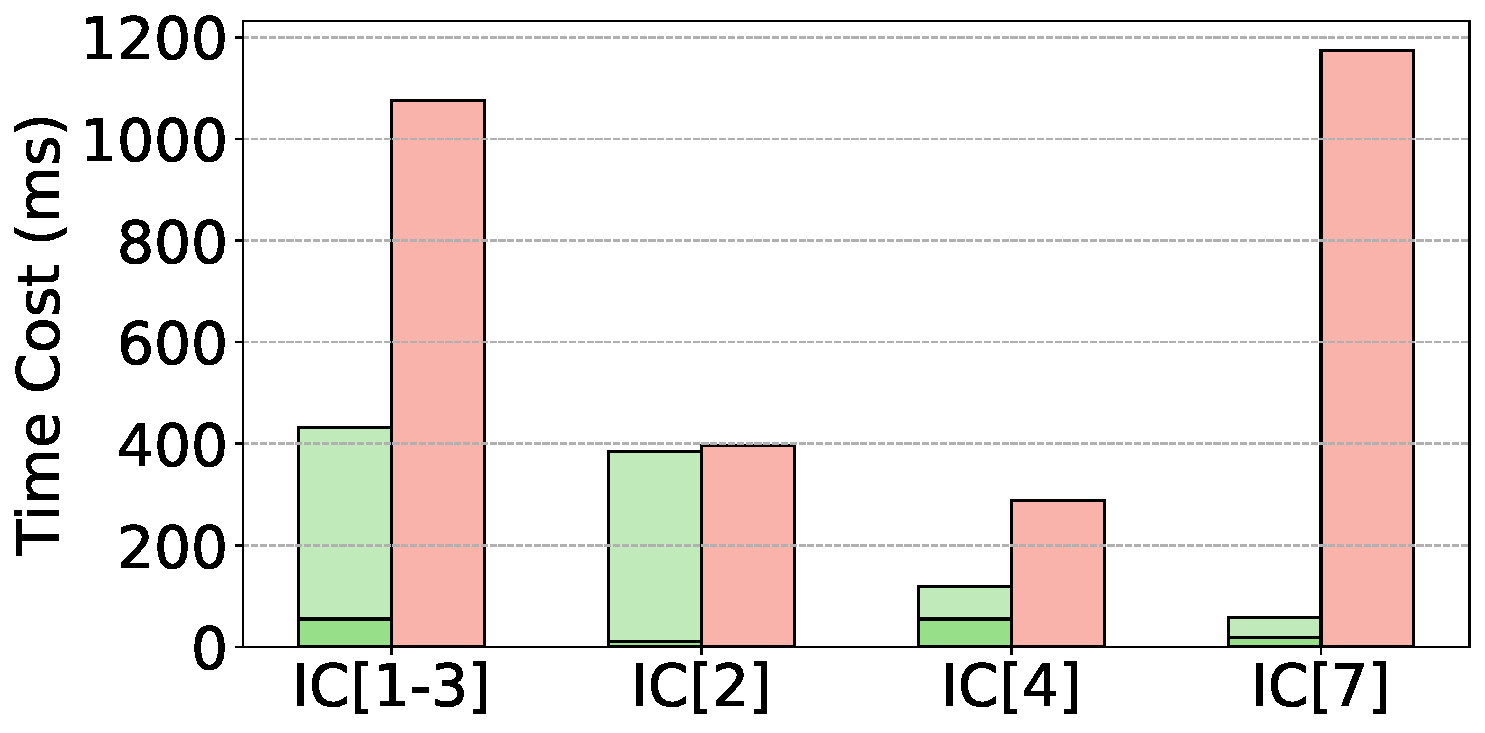
\includegraphics[width=\linewidth]{./figures/exp/opt_exe_ldbc.pdf}
        \vspace{-1.5em}
        \caption{End-to-End Time on $LDBC30$.}
        \label{fig:exp-opt-ldbc}
    \end{subfigure}
    \begin{subfigure}[b]{0.48\linewidth}
        \centering
        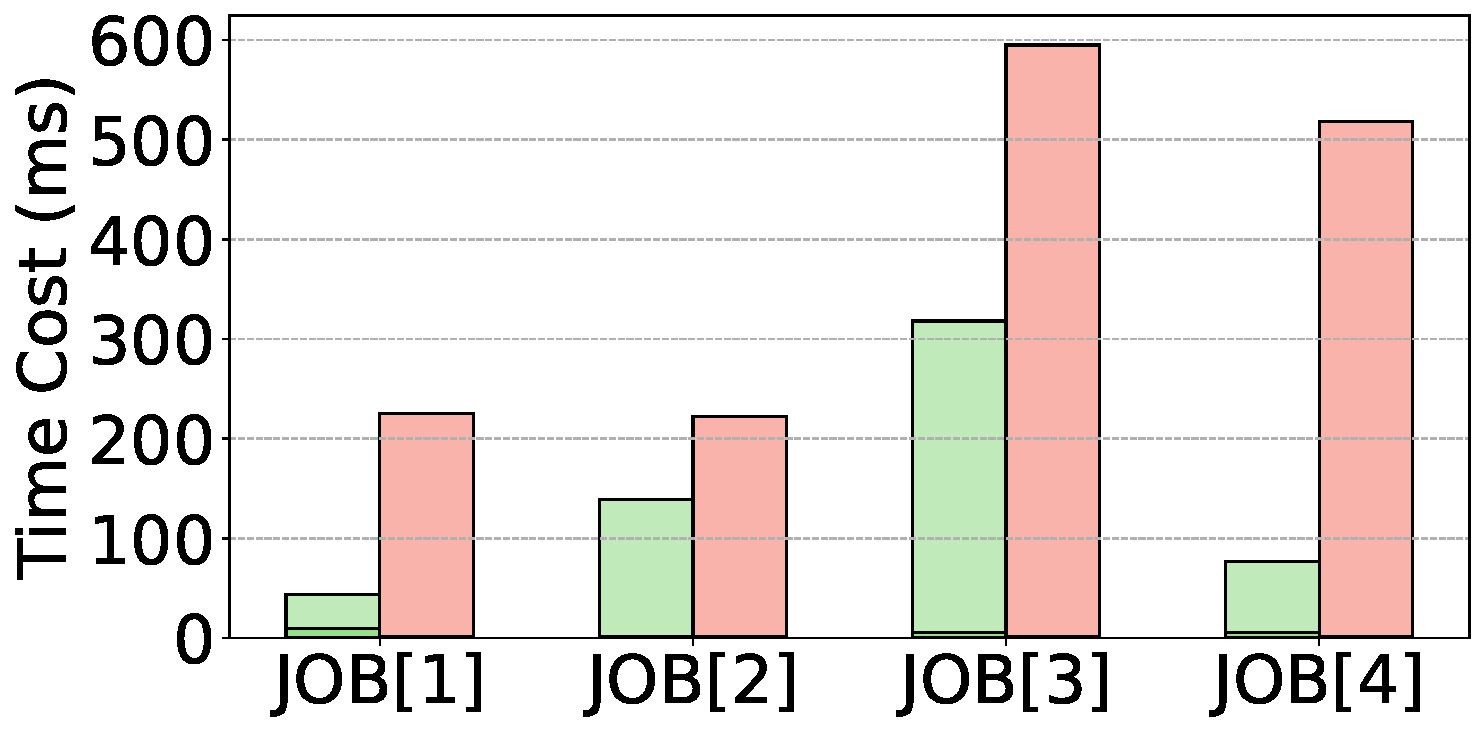
\includegraphics[width=\linewidth]{./figures/exp/opt_exe_job.pdf}
        \vspace{-1.5em}
        \caption{End-to-End Time on IMDB.}
        \label{fig:exp-opt-job}
    \end{subfigure}
    \caption{Experiments on optimization and execution cost}
    \label{fig:exp-optimization}
\end{figure}

% In the experiments, optimizing all the queries with \name can be finished in 10 minutes, while optimizing some queries with Calcite exceeds the 10-minute limit.
% For example, when JOB benchmark is utilized, the time cost of optimizing all the queries with Calcite is longer than 10 minutes.
% As shown in Fig.~\ref{fig:exp-optimization}, \name is much more efficient than Calcite in optimizing queries, and it is consistent with the conclusions obtained in Sec.~\ref{sec:theoretical-analysis}.
% That is, \name is exponentially faster than Calcite in query optimization.
% For instance, when IC5-1 is queried on $LDBC30$, the time cost of query optimization with \name can be more than $10^4\times$ faster than that of Calcite.

% Besides, the optimization time cost of \name is similar on $LDBC10$ and $LDBC30$, and so is Calcite.
% The reason is that the time required for optimization is not significantly associated with the scale of the dataset; instead, it is related to the relative cardinalities among the different tables.
% The relative cardinalities in LDBC datasets of different scales are consistent, therefore the optimization time is similar.

\begin{figure}[ht]
    \vspace{-1em}
    \centering
    \begin{subfigure}[b]{.45\linewidth}
        \centering
        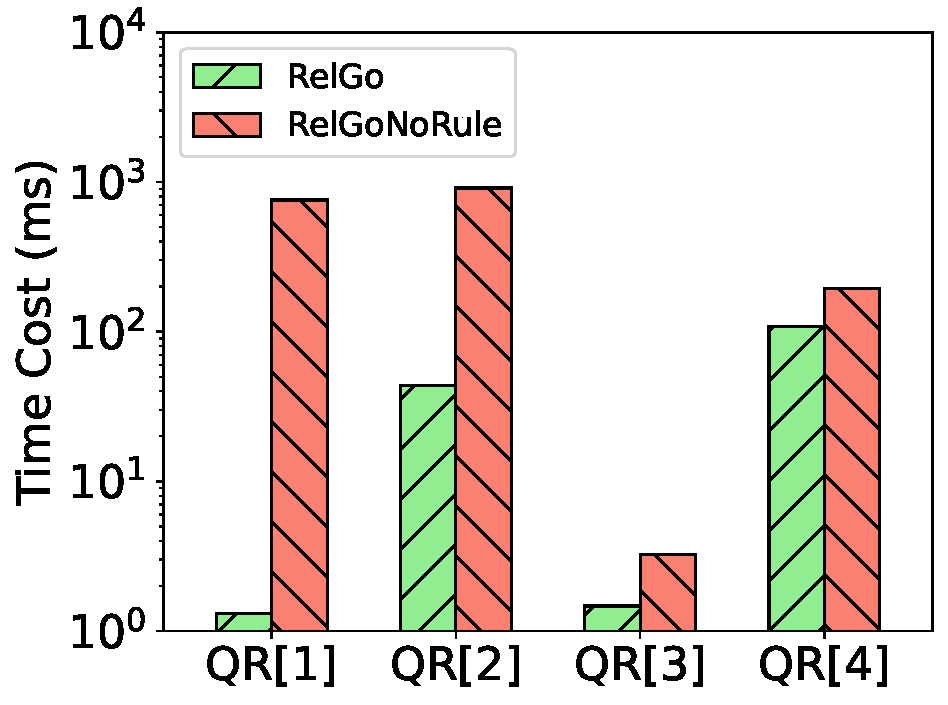
\includegraphics[width=\linewidth]{./figures/exp/filter_sf10.pdf}
        \vspace{-1.5em}
        \caption{Time Cost on $LDBC10$.}
        \label{fig:exp-filter-sf10}
    \end{subfigure}
    \begin{subfigure}[b]{0.45\linewidth}
        \centering
        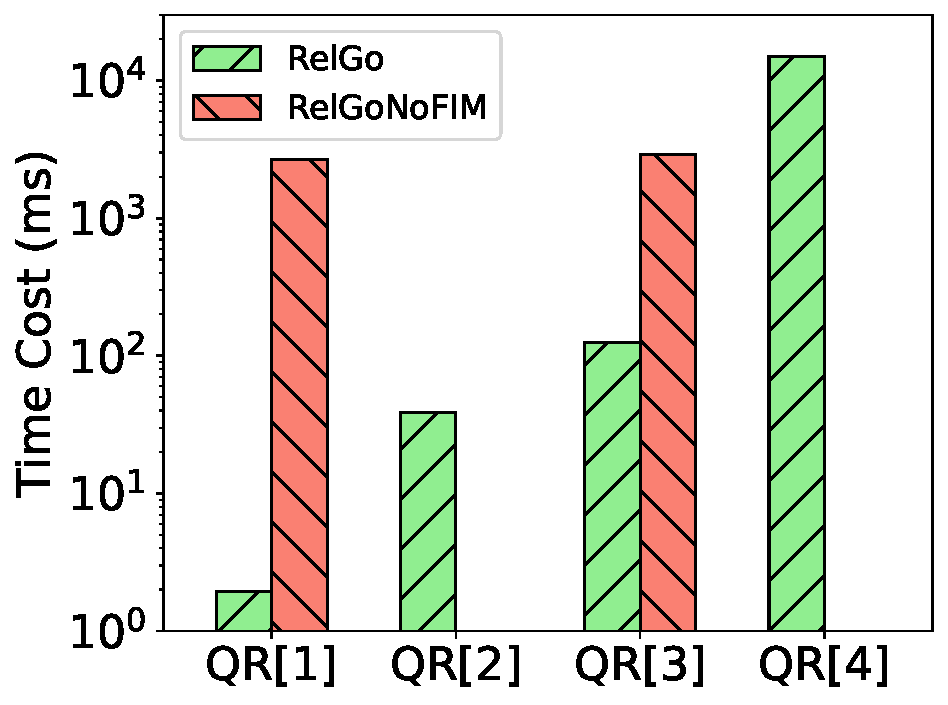
\includegraphics[width=\linewidth]{./figures/exp/filter_sf30.pdf}
        \vspace{-1.5em}
        \caption{Time Cost on $LDBC30$.}
        \label{fig:exp-filter-sf30}
    \end{subfigure}
    \caption{Efficiency comparison of \name and \relgonofi}
    \label{fig:exp-filter}
\end{figure}

\begin{figure}[ht]
    \vspace{-1em}
    \centering
    \begin{subfigure}[b]{.45\linewidth}
        \centering
        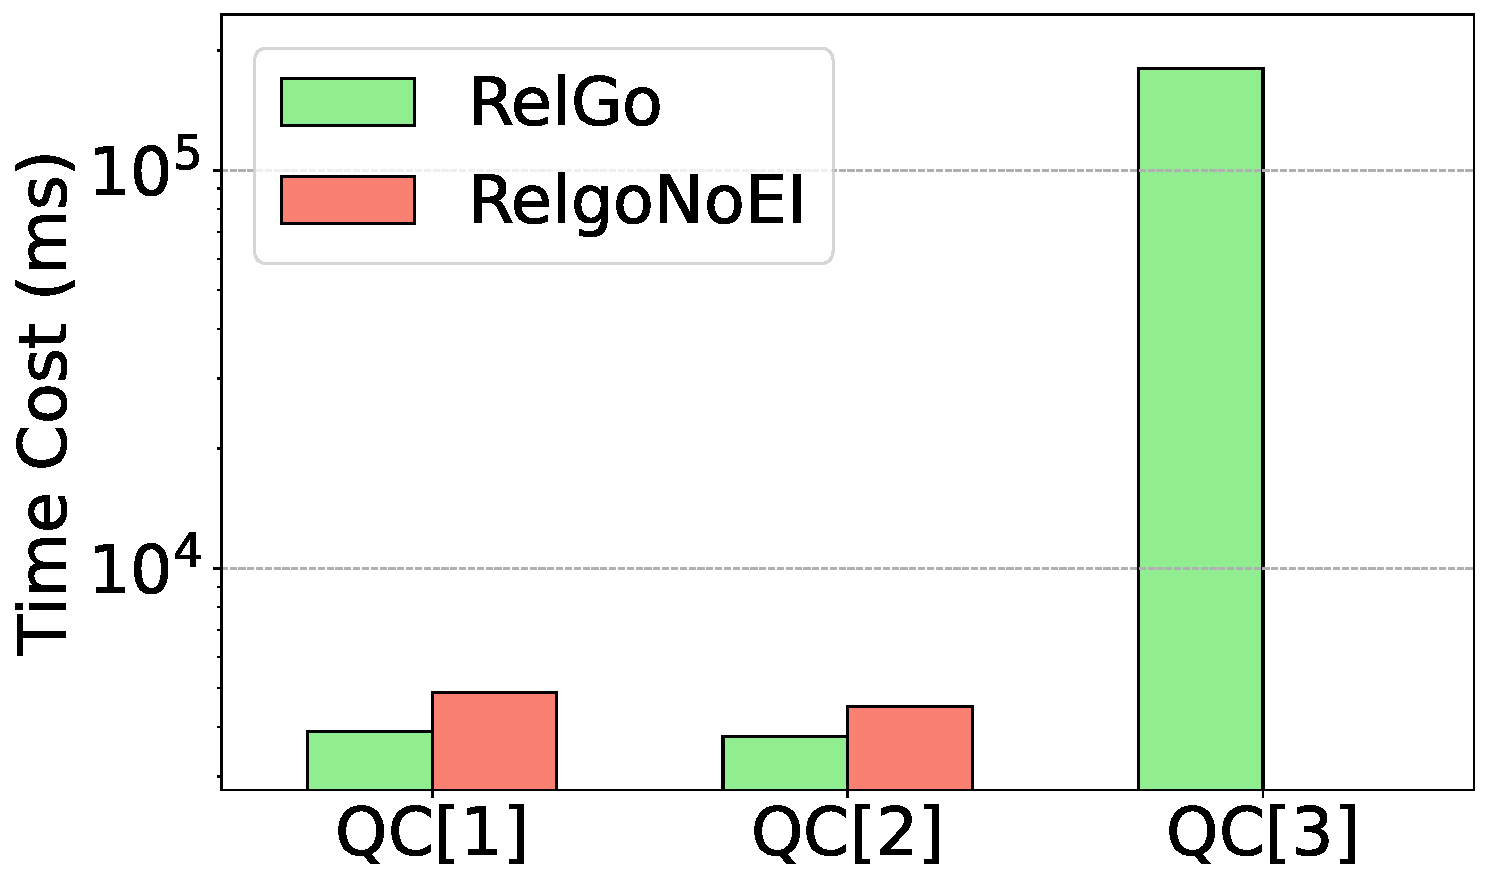
\includegraphics[width=\linewidth]{./figures/exp/ablation_ei_sf10.pdf}
        \vspace{-1.5em}
        \caption{Time Cost on $LDBC10$.}
        \label{fig:exp-expand-intersect-sf10}
    \end{subfigure}
    \begin{subfigure}[b]{0.45\linewidth}
        \centering
        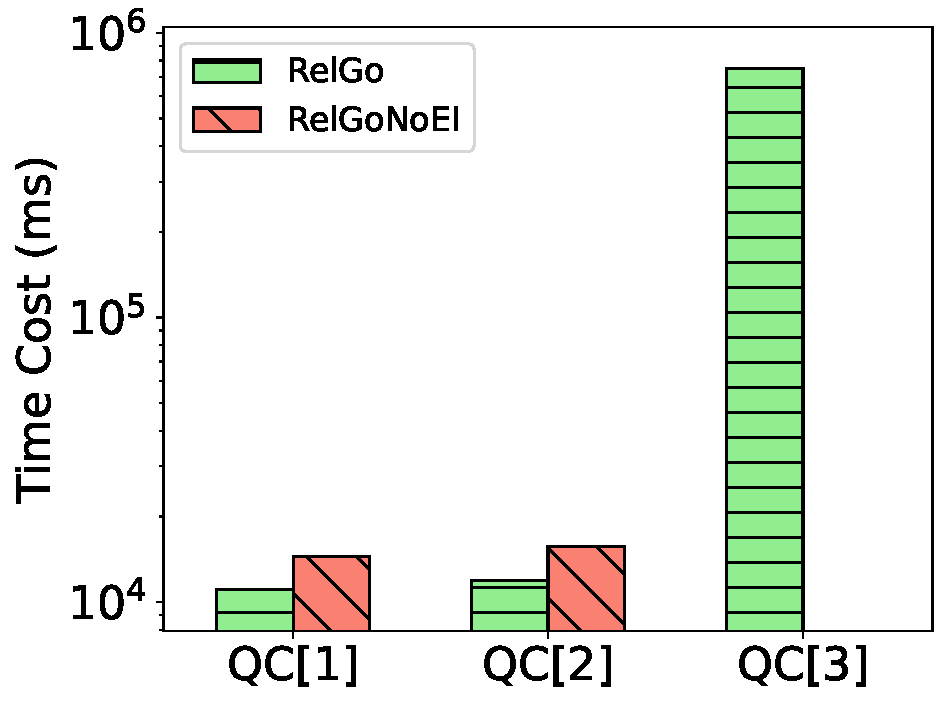
\includegraphics[width=\linewidth]{./figures/exp/ablation_ei_sf30.pdf}
        \vspace{-1.5em}
        \caption{Time Cost on $LDBC30$.}
        \label{fig:exp-expand-intersect-sf30}
    \end{subfigure}
    \caption{Efficiency comparison of \name and \relgomj}
    \label{fig:exp-expand-intersect}
\end{figure}


\noindent\textbf{Advanced Optimization Strategies.}
In this experiment, we assessed the advanced optimization strategies in \name, including the heuristic \filterrule and \joinfuserule, and the optimized implementation of \expandintersect~ operator that aims to improve the efficiency of complete star join.

We began by testing \filterrule and \joinfuserule, two representative heuristic rules employed in \name that capture optimization opportunities at the interplay of relational and graph optimizations. We conducted experiments on $LDBC10$ and $LDBC30$, using $QR[1]$ and $QR[2]$ to evaluate \filterrule, and $QR[3]$ and $QR[4]$ to test \joinfuserule. The results, depicted in \reffig{exp-filter}, compared the performance of \name with and without applying these rules, denoted as \name and \relgonofi, respectively.
The results demonstrate that \filterrule significantly improves query performance, providing an average speedup of 299.4$\times$ on $LDBC10$ and 699.8$\times$ on $LDBC30$. After applying \joinfuserule, query execution is accelerated by an average of 2.0$\times$ on $LDBC10$ and 2.3$\times$ on $LDBC30$. These findings suggest that the heuristic rules, particularly \filterrule, are highly effective in enhancing query execution efficiency.

%\enlargethispage{1em}

Next, we evaluated the effectiveness of the \expandintersect, which focuses on improving the efficiency of complete star join. Without this optimization strategy, the \expandintersect~ operator would be implemented as a traditional multiple join, and we denote this variant as \relgomj. We conducted this experiment with queries $QC[1 \ldots 3]$ that contain cycles and compared the performance of \name and \relgomj.
The performance results, depicted in \reffig{exp-expand-intersect}, suggest that, compared to \relgomj, \name achieves an average speedup of 1.22$\times$ on $LDBC10$ and 1.31$\times$ on $LDBC30$ (excluding $QC[3]$). Notably, for $QC[3]$, which is a complex 4-clique, the plans optimized by \relgomj confront an out-of-memory (OOM) error. %The reason is that applying worst-case optimal joins generates significantly fewer intermediate results than applying multiple joins, as numerous results that will not appear in the intersection are prematurely eliminated.
The results of this experiment indicate that the \expandintersect~ operator with an optimized implementation not only enhances query performance but also significantly reduces the spatial overhead.

\begin{figure}[ht]
    \centering
    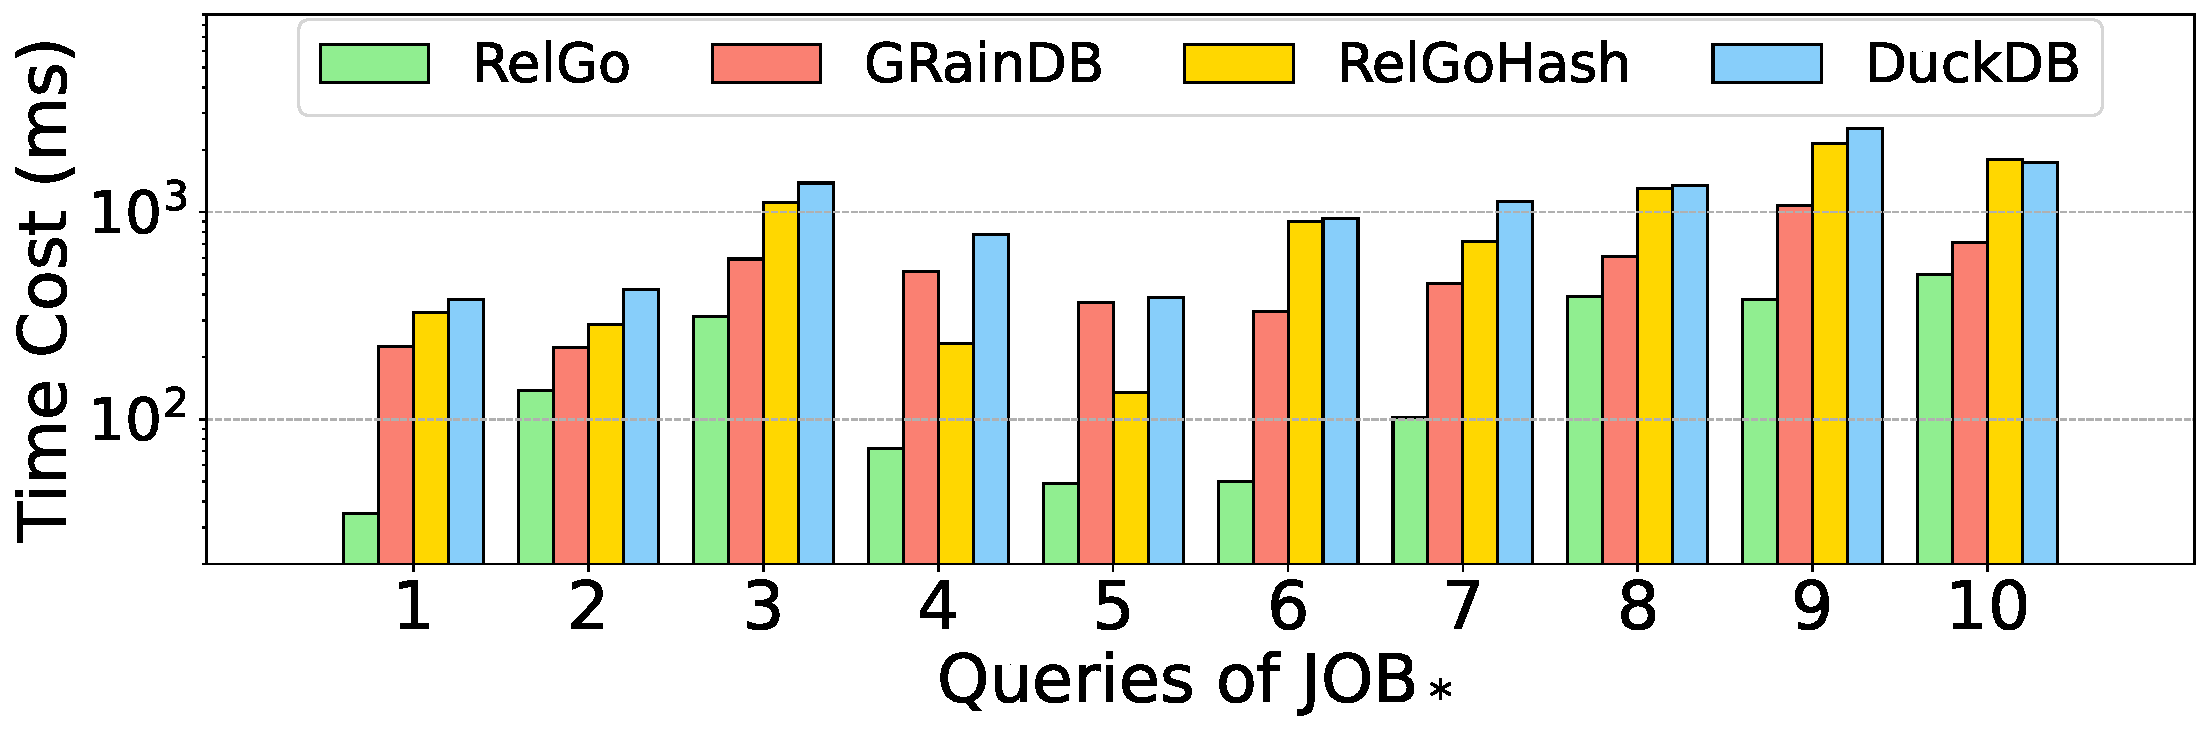
\includegraphics[width=\linewidth]{./figures/exp/hash_plan_job.pdf}
    \caption{Experiments on join order efficiency}
    \label{fig:exp-hash-plan}
\end{figure}

\noindent\textbf{Efficiency of Join Order.}
%After the assessment of advanced strategies within \name, we integrate all these strategies (and so as in the following experiments) to conduct a performance comparison between \name, GrainDB, and DuckDB with a focus on the join order efficiency.
In this experiment, we compared \name with GrainDB and DuckDB, focusing on the efficiency of the join order. For this purpose, we introduced a variant of \name called \relgohash, which optimizes the plan in a converged manner like \name but deliberately bypasses the use of graph index. We selected 10 queries from the JOB benchmark and showed the performance results in \reffig{exp-hash-plan}.
The results demonstrate that \name outperforms GrainDB on all the queries, accelerating the execution time by factors ranging from \revise{$1.4\times$} to $7.5\times$, with an average speedup of \revise{$4.14\times$}. Additionally, the plans optimized with \relgohash are at least as good as those optimized by DuckDB, achieving an average speedup of \revise{$1.6\times$}. The effectiveness of \name and \relgohash stems from their use of advanced graph-aware optimization techniques in optimizing the matching operator, resulting in good join order and thus robust performance regardless of the presence or absence of graph index.
It is worth noting that \name does not always generate plans with the absolute best join orders, as it relies on the estimated cost of the plans. However, its optimized plans generally remain competitive in most cases, thanks to its integration of \glogue that use high-order statistics for cost estimation.

%This superior join order offsets the absence of graph indices in the execution process.

% In this section, we conduct ablation study to show the efficiency of \expandintersectrule.
% In detail, patterns in Fig.~\ref{fig:exp-hard-patterns} are queried on $LDBC10$ and $LDBC30$, and plans are optimized with Relgo.
% For each plan optimized by Relgo, we replace the extend-intersect operators in it with multiple join operators and obtain a new plan.
% These new plans are called obtained with \textit{"Relgo w.o. EI"}.
% The experimental results are shown in Fig.~\ref{fig:exp-ablation-ei}.

% The results illustrate the efficiency of \expandintersectrule.
% When triangles are searched for, removing the extend-intersect operators decreases the query performance.
% Besides, when butterflies and 4-cliques are searched for, the plans without extend-intersect operators have an excessive memory overhead and cause an ``Out of Memory'' (abbr.~OOM) error.
% The reason is that applying extend-intersect operators has much fewer intermediate results than applying multiple joins, since numerous results that will not appear in the intersection are prematurely deleted.
% It indicates that \expandintersectrule can not only enhance query performance, but also reduce spatial overhead.

% To further demonstrate the efficiency of \expandintersectrule, we add predicates on butterflies (i.e., Fig.~\ref{fig:exp-hard-butterfly}) and 4-cliques (i.e., Fig.~\ref{fig:exp-hard-clique}) to avoid OOM, and generate two new patterns, i.e., \textit{Butterfly-P} and \textit{4-Clique-P}.
% Specifically, for these two new patterns, the values of properties Person1.\textit{p\_personid} are constrained to be smaller than specified values.
% Queries of these new patterns are optimized with GrainDB, \name, and \textit{\name w.r. EI}.
% The results on the constrained-patterns are shown in Fig.~\ref{fig:exp-ablation-para-ei}.


% The results suggest that \expandintersectrule is crucial in optimizing queries with cycles.
% Specifically, for the new patterns with cycles, the execution time of plans optimized by \name is more than an order of magnitude shorter than those optimized by \textit{"Relgo w.o. EI"}.
% It indicates the effectiveness of \expandintersectrule.
% Moreover, when patterns with many cycles are used (e.g., 4-clique in Fig.~\ref{fig:exp-hard-clique}), the optimization effect of the rule becomes particularly noticeable.
% In detail, querying for 4-cliques with \name can be 100$\times$ faster than with \textit{"Relgo w.o. EI"}.
% The results illustrate the efficiency of \expandintersectrule.

\begin{figure}[ht]
    \centering
    \begin{subfigure}[b]{\linewidth}
        \centering
        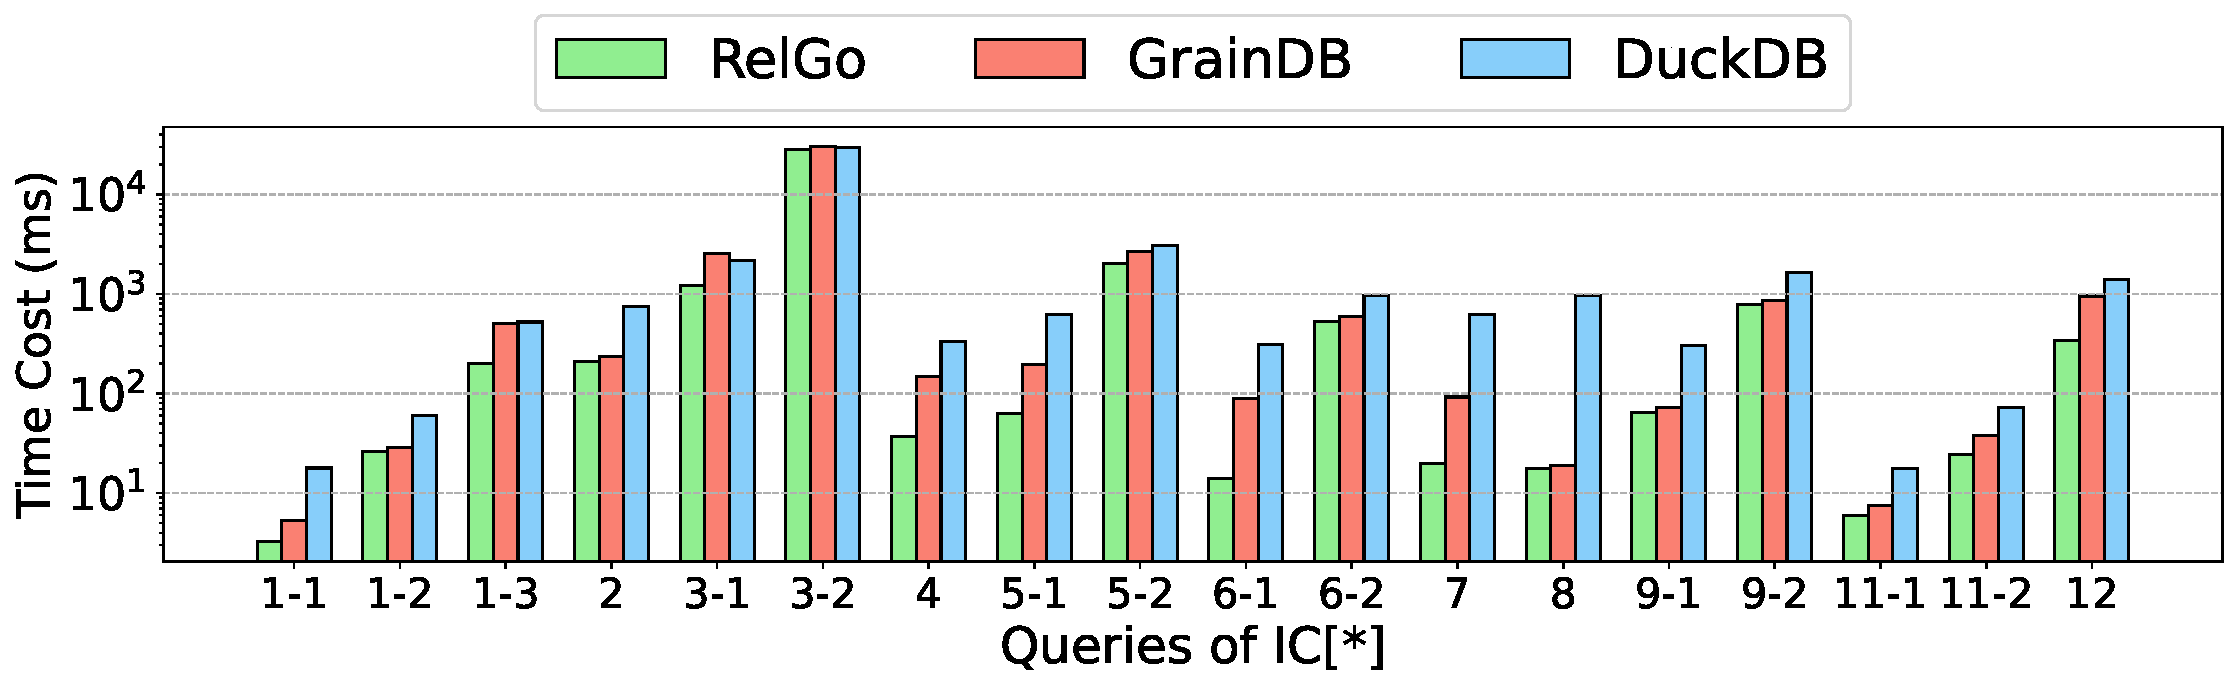
\includegraphics[width=\linewidth]{./figures/exp/e2e_sf10.pdf}
        \vspace{-2em}
        \caption{Speedup Compared to DuckDB on $LDBC10$.}
        \label{fig:exp-e2e-sf10}
    \end{subfigure}
    \begin{subfigure}[b]{\linewidth}
        \centering
        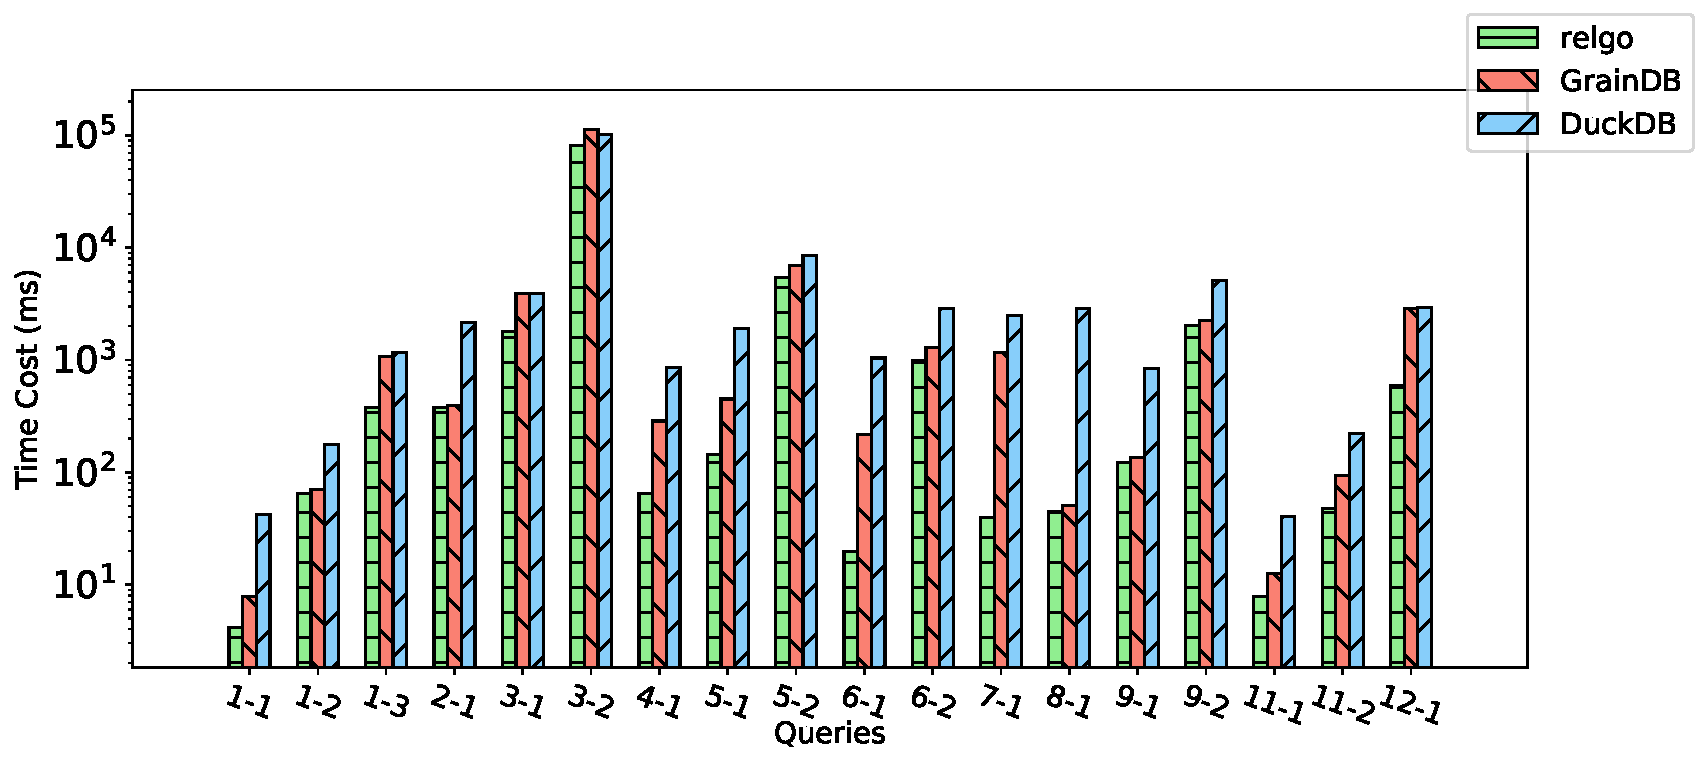
\includegraphics[width=\linewidth]{./figures/exp/e2e_sf30.pdf}
        \vspace{-2em}
        \caption{Speedup Compared to DuckDB on $LDBC30$.}
        \label{fig:exp-e2e-sf30}
    \end{subfigure}
    \begin{subfigure}[b]{\linewidth}
        \centering
        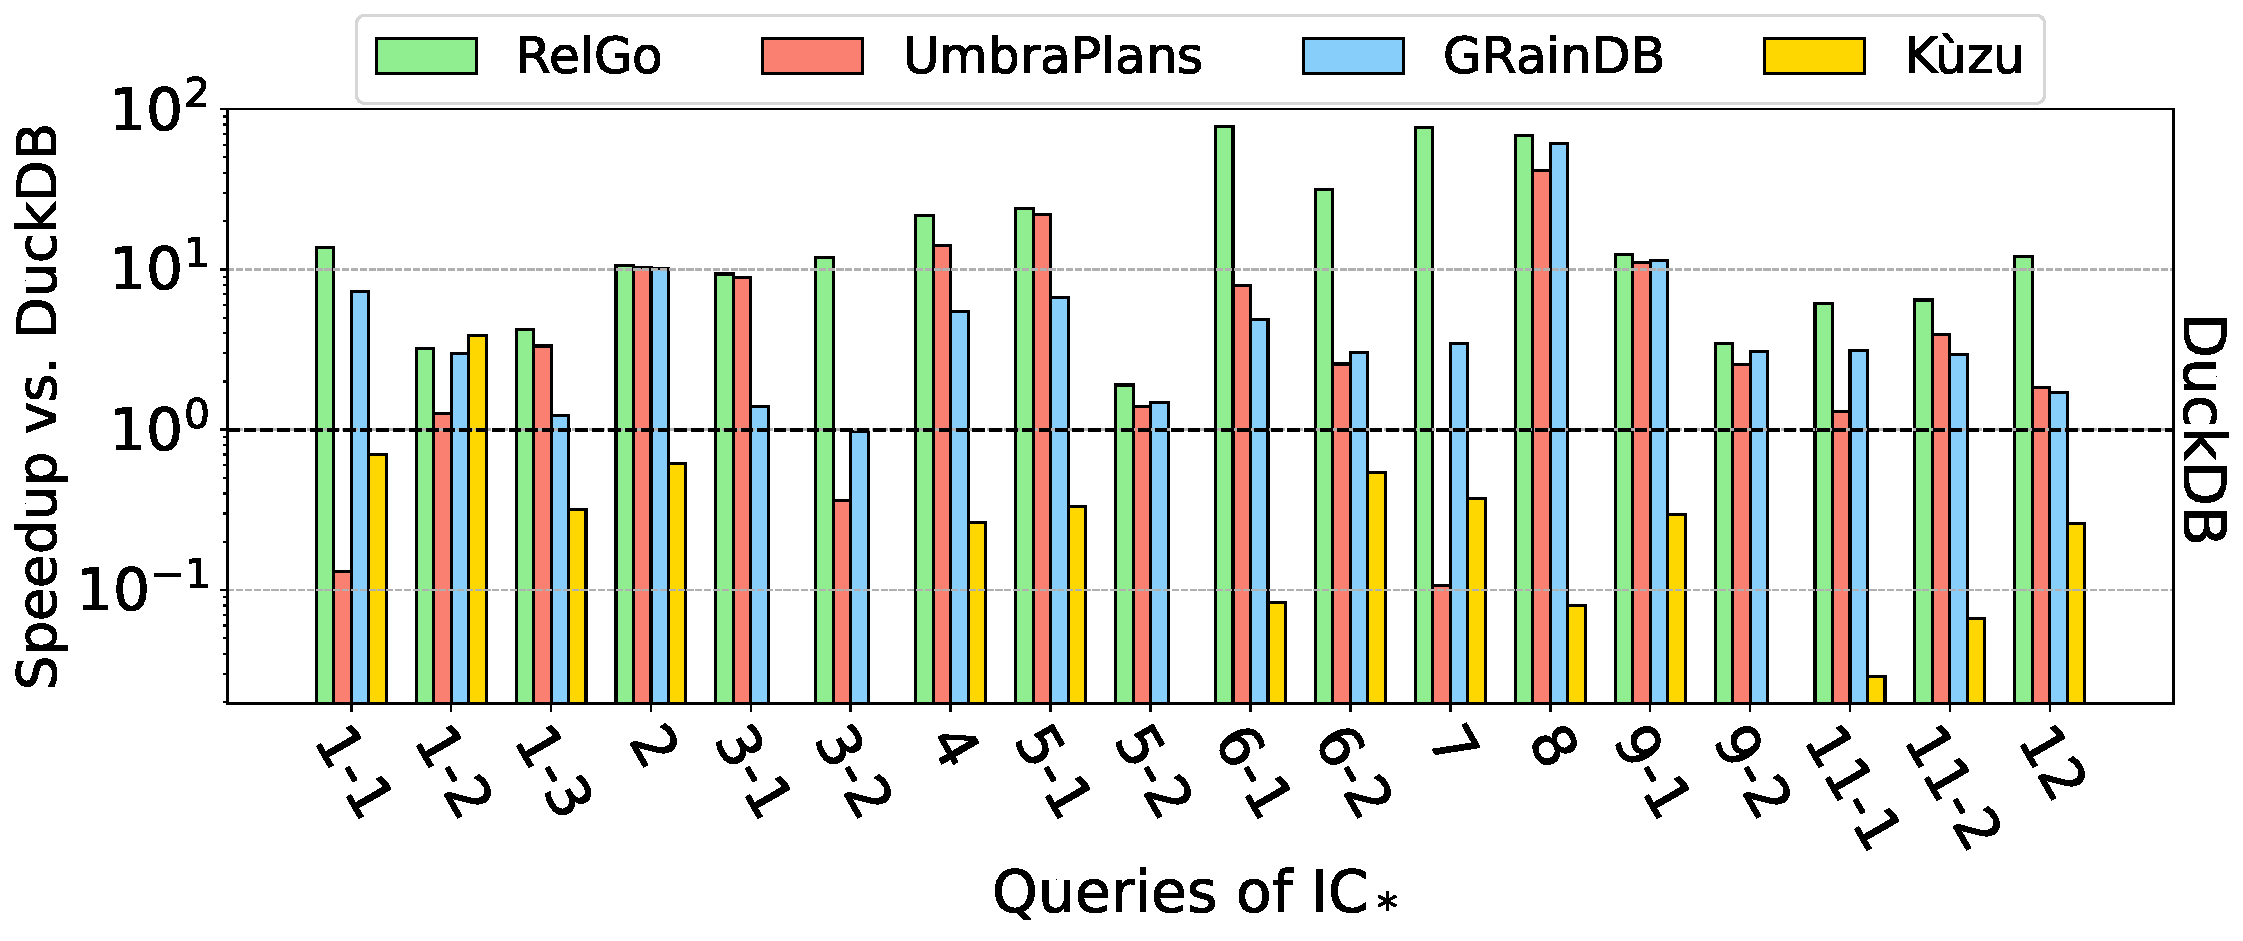
\includegraphics[width=\linewidth]{./figures/exp/e2e_sf100.pdf}
        \vspace{-2em}
        \caption{Speedup Compared to DuckDB on $LDBC100$.}
        \label{fig:exp-e2e-sf30}
    \end{subfigure}
    \begin{subfigure}[b]{\linewidth}
        \centering
        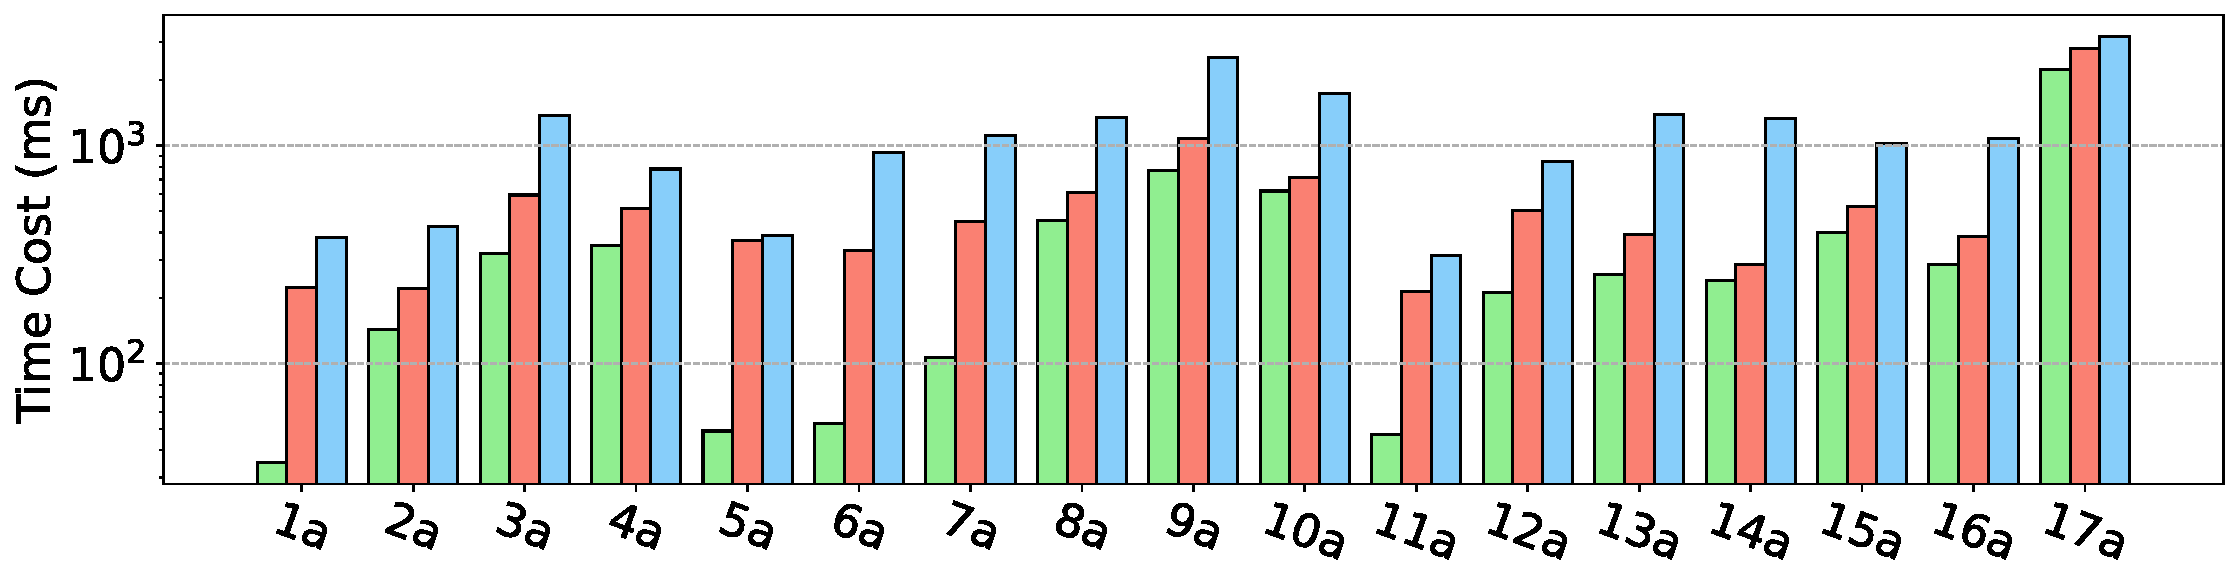
\includegraphics[width=\linewidth]{./figures/exp/e2e_job_part1.pdf}
        \vspace*{-2ex}
    \end{subfigure}
    \begin{subfigure}[b]{\linewidth}
        \centering
        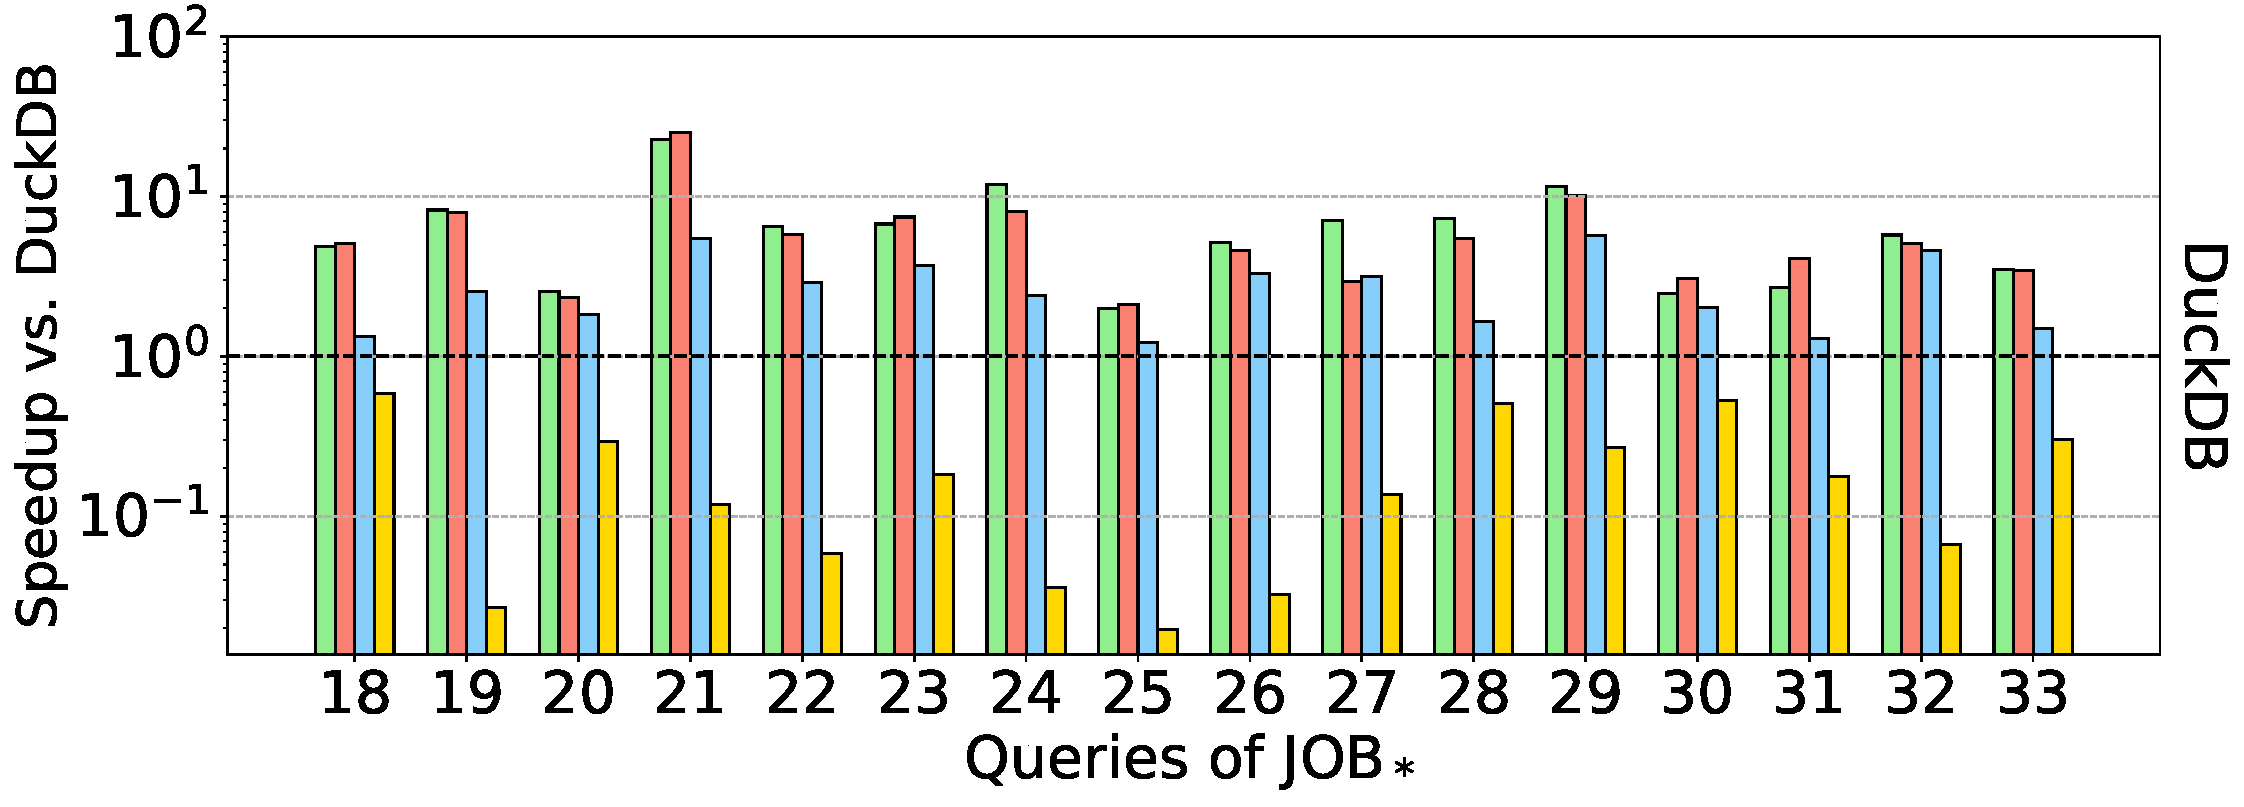
\includegraphics[width=\linewidth]{./figures/exp/e2e_job_part2.pdf}
        \vspace{-2em}
        \caption{Speedup Compared to DuckDB on IMDB.}
        \label{fig:exp-e2e-job}
    \end{subfigure}
    \caption{Results of the comprehensive experiments. The speedup of method A compared to DuckDB is computed as $\frac{\text{Time}(DuckDB)}{\text{Time}(A)}$. Note that the results of Kùzu are sometimes omitted (e.g., IC[3-1] and IC[3-2] on $LDBC10$) due to out-of-memory errors (abbr.~OOM).}
    \label{fig:exp-e2e}
\end{figure}

\subsection{Comprehensive Experiments}
\label{sec:experiment-e2e}


We conducted comprehensive experiments on the LDBC and JOB benchmarks to comprehensively evaluate the performance of \name compared to \revise{the baselines, i.e., Umbra, GrainDB, DuckDB, and Kùzu}. The experimental results, presented in \reffig{exp-e2e}, demonstrate that execution plans optimized by \name consistently \revise{outperform those optimized by the baselines on both benchmarks}.
Specifically, for the LDBC benchmark, the execution time of the plans optimized by \name is about \revise{22.4$\times$}, \revise{5.0$\times$}, \revise{12.4$\times$} and \revise{77.4$\times$} faster on average than those generated by Umbra, GrainDB, DuckDB and Kùzu \revise{(OOM queries discarded)}, respectively, on $LDBC10$, about \revise{37.6$\times$}, \revise{6.6$\times$}, \revise{17.9$\times$} and \revise{125.9$\times$} faster on $LDBC30$, \revise{and about 49.9$\times$, 5.4$\times$, 21.9$\times$ and 188.68$\times$ on $LDBC100$}. It is important to note that \name is especially effective for queries containing cycles, which can benefit more from graph optimizations. For example, in query $IC[7]$, which contains a cycle, \name outperforms Umbra, GrainDB, DuckDB and Kùzu by \revise{578.6$\times$, 29.7$\times$, 63.5$\times$ and 162.0$\times$}, respectively, on $LDBC30$.
Conversely, the JOB benchmark, established for assessing join optimizations in relational databases, lacks any cyclic-pattern queries. Despite this, \name still achieves better performance compared to Umbra, GrainDB, DuckDB and Kùzu, with an average speedup of \revise{1.7$\times$, 4.0$\times$, 8.2$\times$ and 136.1$\times$}, respectively.

%\enlargethispage{1em}

The experiment results reflect our discussions in \refsec{graph-aware}. We summarize the superiority of \name as follows.
First, \name is designed to be aware of the existence of graph index in query optimization and can leverage the index to effectively retrieve adjacent edges and vertices. In contrast, for \revise{Umbra and GrainDB}, relational optimizers can occasionally alter the order of \EVjoin operations, rendering graph index ineffective. DuckDB, on the other hand, does not consider graph index in query optimization and executes queries using conventional hash joins, which are often less efficient compared to graph-aware approaches.
Second, by incorporating a matching operator in \spjm queries to capture the graph query semantics, \name is able to leverage advanced graph optimization techniques to optimize the matching operator. These techniques include using high-order statistics to estimate the cost of plans more accurately and employing worst-case optimal join implementations to optimize cyclic patterns. In contrast, DuckDB and GrainDB cannot benefit from these graph-specific optimizations, which may lead to suboptimal plans and inefficient execution.
\revise{Although Umbra's optimizer supports generating execution plans that include multiway joins, in our actual experiments, none of the optimized plans for the queries contained multiway joins. This indicates that Umbra also struggles to leverage the graph-specific optimizations}.
Third, \name considers optimization opportunities across both graph and relational query semantics, introducing effective heuristic rules such as \filterrule and \joinfuserule. These rules can significantly improve the efficiency of the generated plans.


Notably, \revise{there are instances where Umbra generates better execution plans compared to \name, e.g., when JOB[30] is queried on IMDB, the execution time of the plan generated by \name is about 1.2$\times$ that of Umbra. A possible reason is that the distributions of attribute values are not yet considered in \name and the Umbra can sometimes estimate cardinalities more accurately when predicates exist.
We consider this as our further work}.

Moreover, \revise{there is an inevitable gap between relational data and graph data. One important distinction is that not every relation can be clearly identified as either a vertex relation or an edge relation. For example, in the JOB dataset, some tables contain more than two foreign keys, and some of these foreign keys reference the primary key of a vertex relation, making it difficult to definitively classify them as either vertex or edge relations. Another important difference is that joins between relational tables can occur in any order, whereas in plans generated by graph optimizers, vertex relations and edge relations need to alternate. Therefore, the relational optimizer has a larger search space, which can sometimes lead to better results.}

This \revise{problem can be addressed by extending \name to \hyname, a hybrid optimizer that processes SPJ queries as inputs. Utilizing pre-existing graph indices, \hyname determines whether tuples in a relational table can be converted to edges in a graph. An intuitive method for converting relational tables to vertices and edges is provided by Boudaoud \cite{Boudaoud2022}. Given an SPJ query, \hyname transforms arbitrary relational tables into vertices or edges, thereby converting the original SPJ query into an SPJM query. Each matching operator within this query contains a connected pattern graph. The results produced by these matching operators are then joined to yield the final results. Since the costs of matching and relational operators are computable, \hyname explores various methods for transforming relational tables into vertices and edges to identify the optimal execution plan, and more cost-based global optimization rules can be designed. Meanwhile, extensive global optimizations can lead to increased optimization time overhead. Therefore, it is necessary to carefully balance and select appropriate global and local optimization rules based on the specific circumstances.
We plan to implement \hyname in the future}.

% There are mainly two reasons for the superiority of \name.
% Firstly, \name is aware of the existence of graph indices in graph query optimization.
% Thus, the cost estimation of \name is more accurate and better physical plans can be obtained.
% In contrast, the optimizers of DuckDB and GrainDB are of the types $Rel$ and $Rel^+$, respectively, and are not aware of the graph indices in query optimization phase.
% Therefore, the accuracy of cost estimation is limited.
% Secondly, for queries with cycles (e.g., $IC[7]-1$ on LDBC), \name have a superior performance due to the advanced extend-intersect operators, which outperforms the traditional multiple join operators used by DuckDB and GrainDB.
% Such an operator can significantly reduce the time consumption, which is also demonstrated through experiments in \reffig{exp-expand-intersect}.
% \todo{update this, with the new TrimFusionRule:} Thirdly, \name is more adept at identifying opportunities to effectively utilize graph indices to get neighbors of vertices, since it optimizes graph queries from the graph perspective.
% Conversely, GrainDB occasionally partitions the process into separate stages, first retrieving adjacent edges and subsequently obtaining the corresponding endpoints.

\begin{figure}[ht]
    \centering
    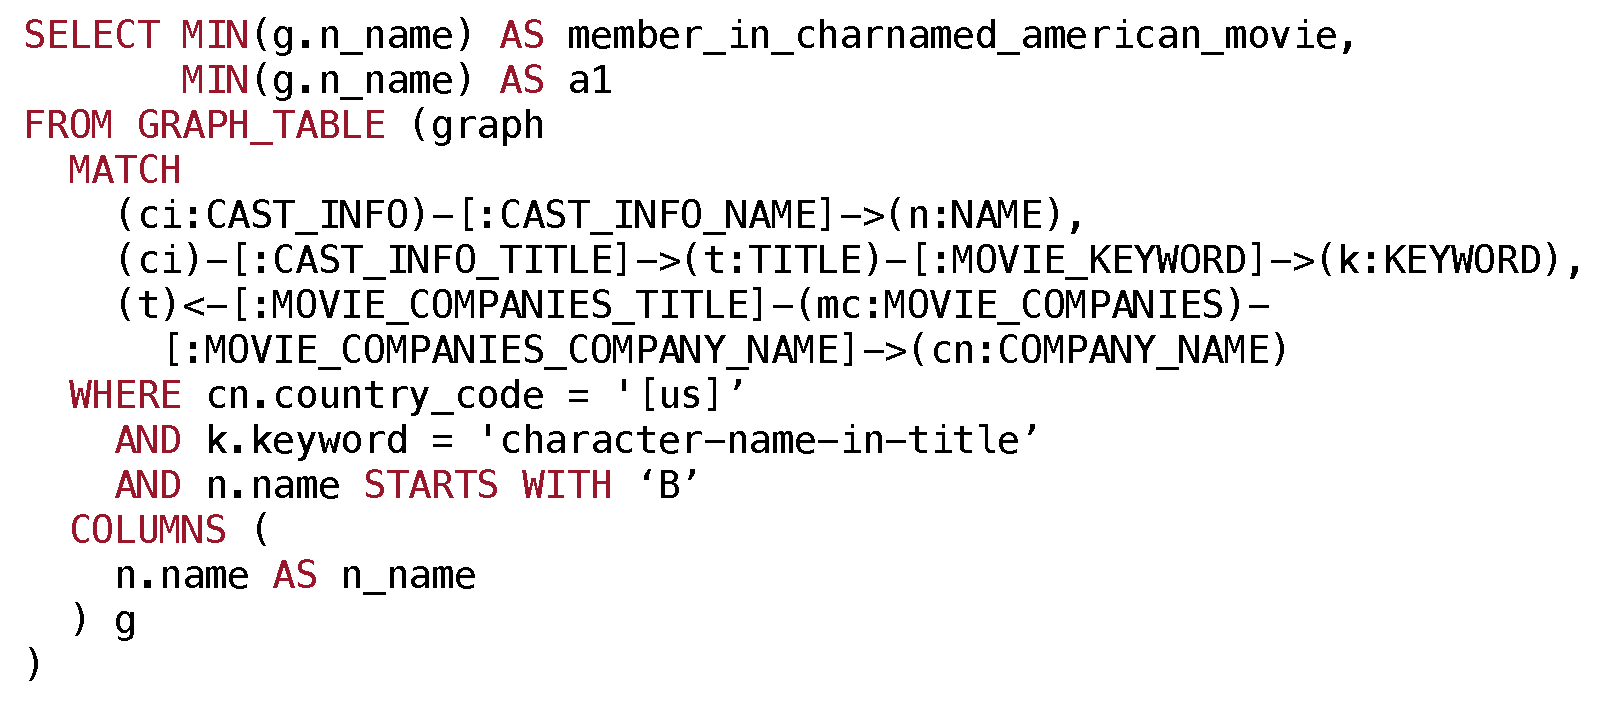
\includegraphics[width=\linewidth]{./figures/job17a-query.pdf}
    \caption{JOB[17] query.}
    \label{fig:job17-query}
\end{figure}


\begin{figure*}[ht]
    \centering
    \begin{subfigure}[b]{.3\linewidth}
        \centering
        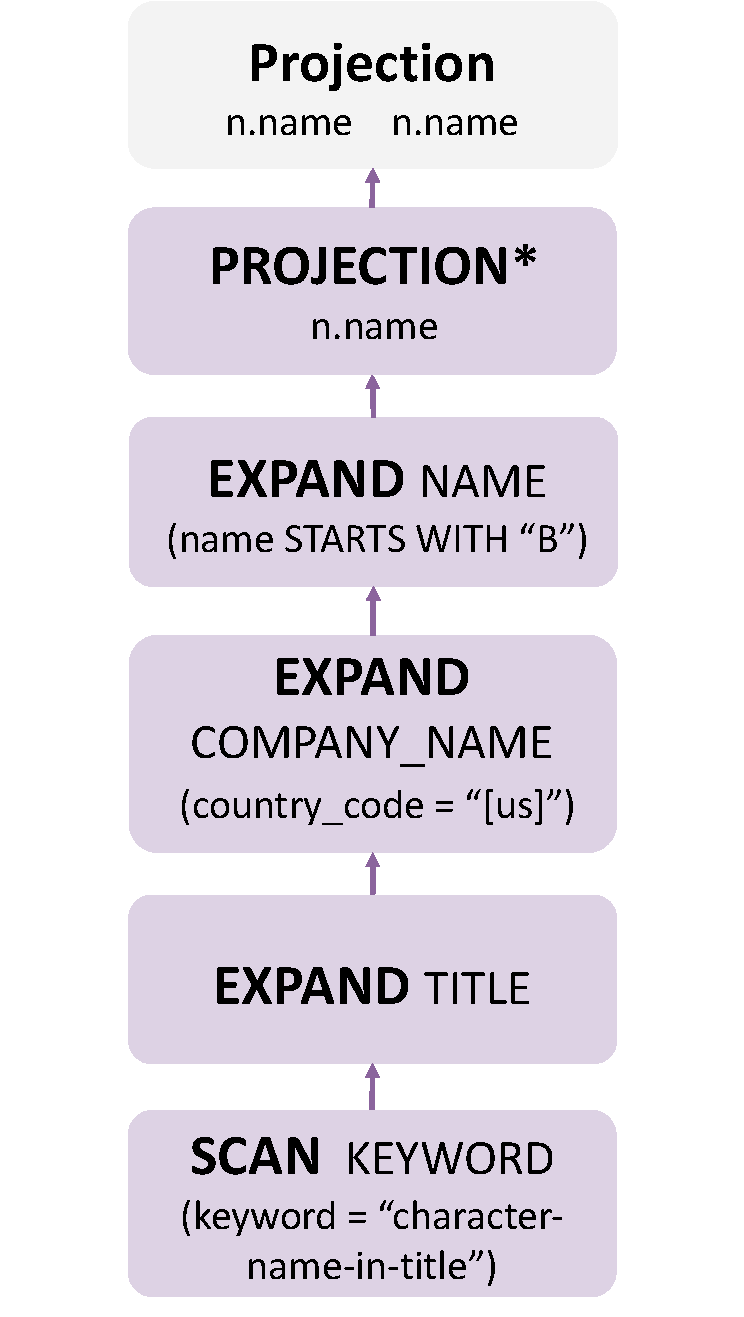
\includegraphics[width=.9\linewidth]{./figures/job17a-plan-gopt.pdf}
        \caption{Query Plan of \name.}
        \label{fig:job17a-plan-relgo}
    \end{subfigure}
    \begin{subfigure}[b]{.25\linewidth}
        \centering
        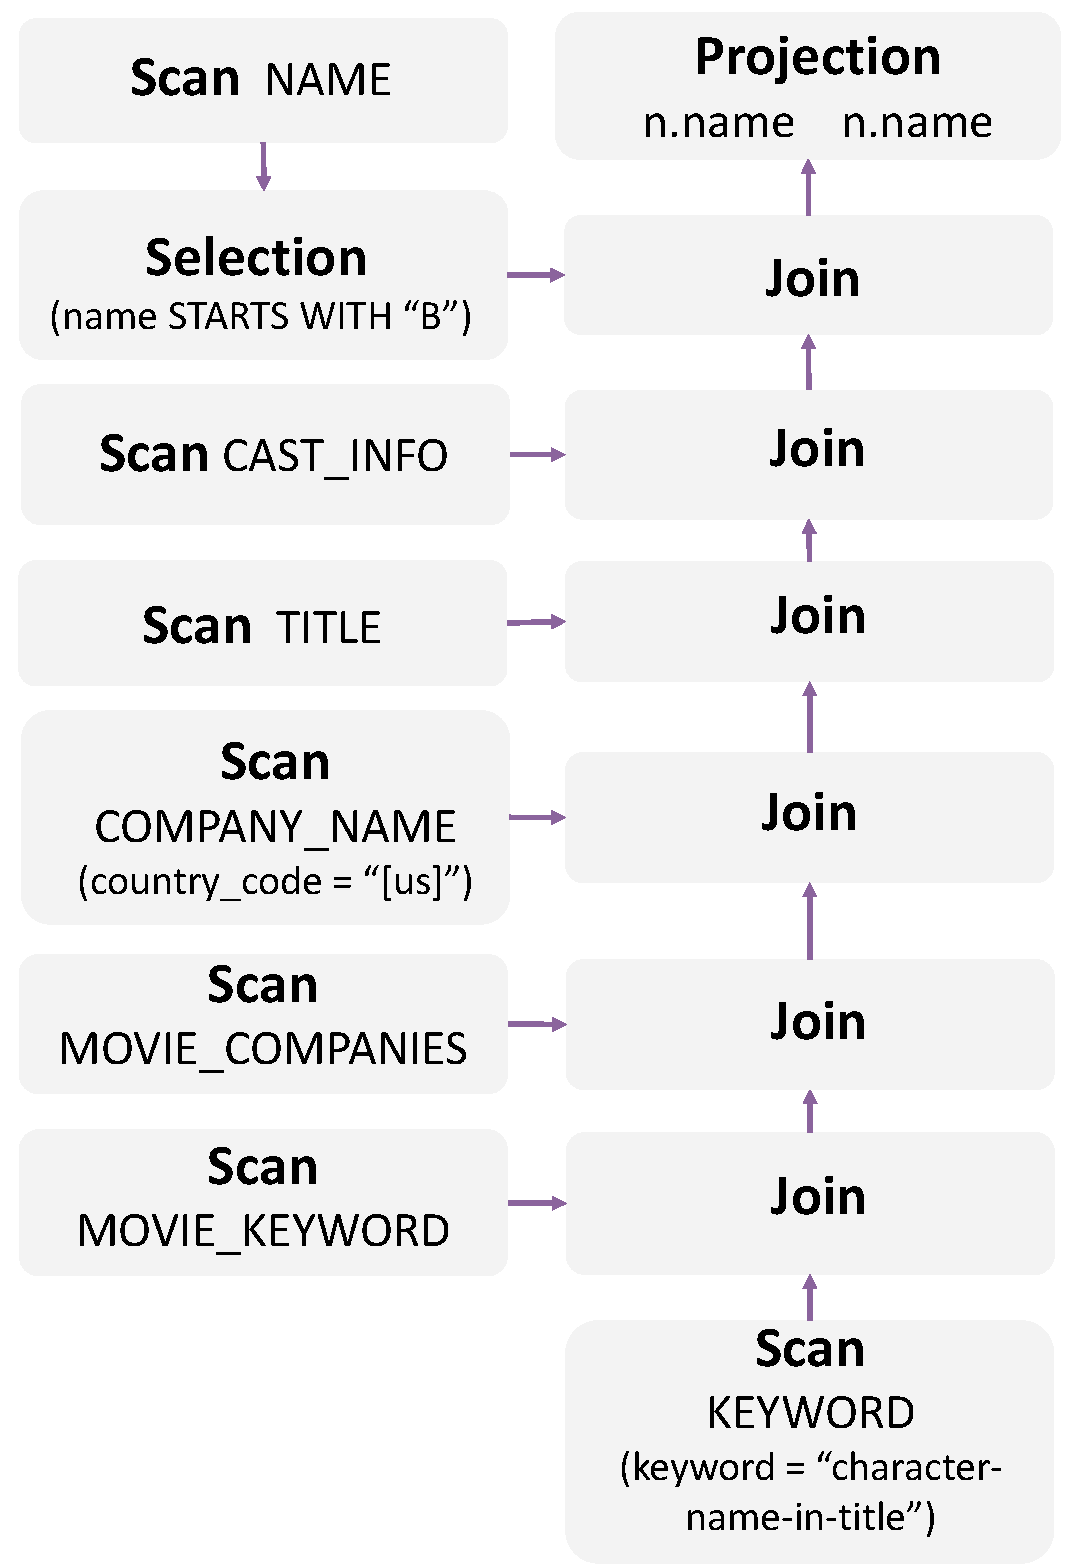
\includegraphics[width=.95\linewidth]{./figures/job17a-plan-graindb.pdf}
        \caption{Query Plan of GrainDB.}
        \label{fig:job17a-plan-graindb}
    \end{subfigure}
    \begin{subfigure}[b]{.4\linewidth}
        \centering
        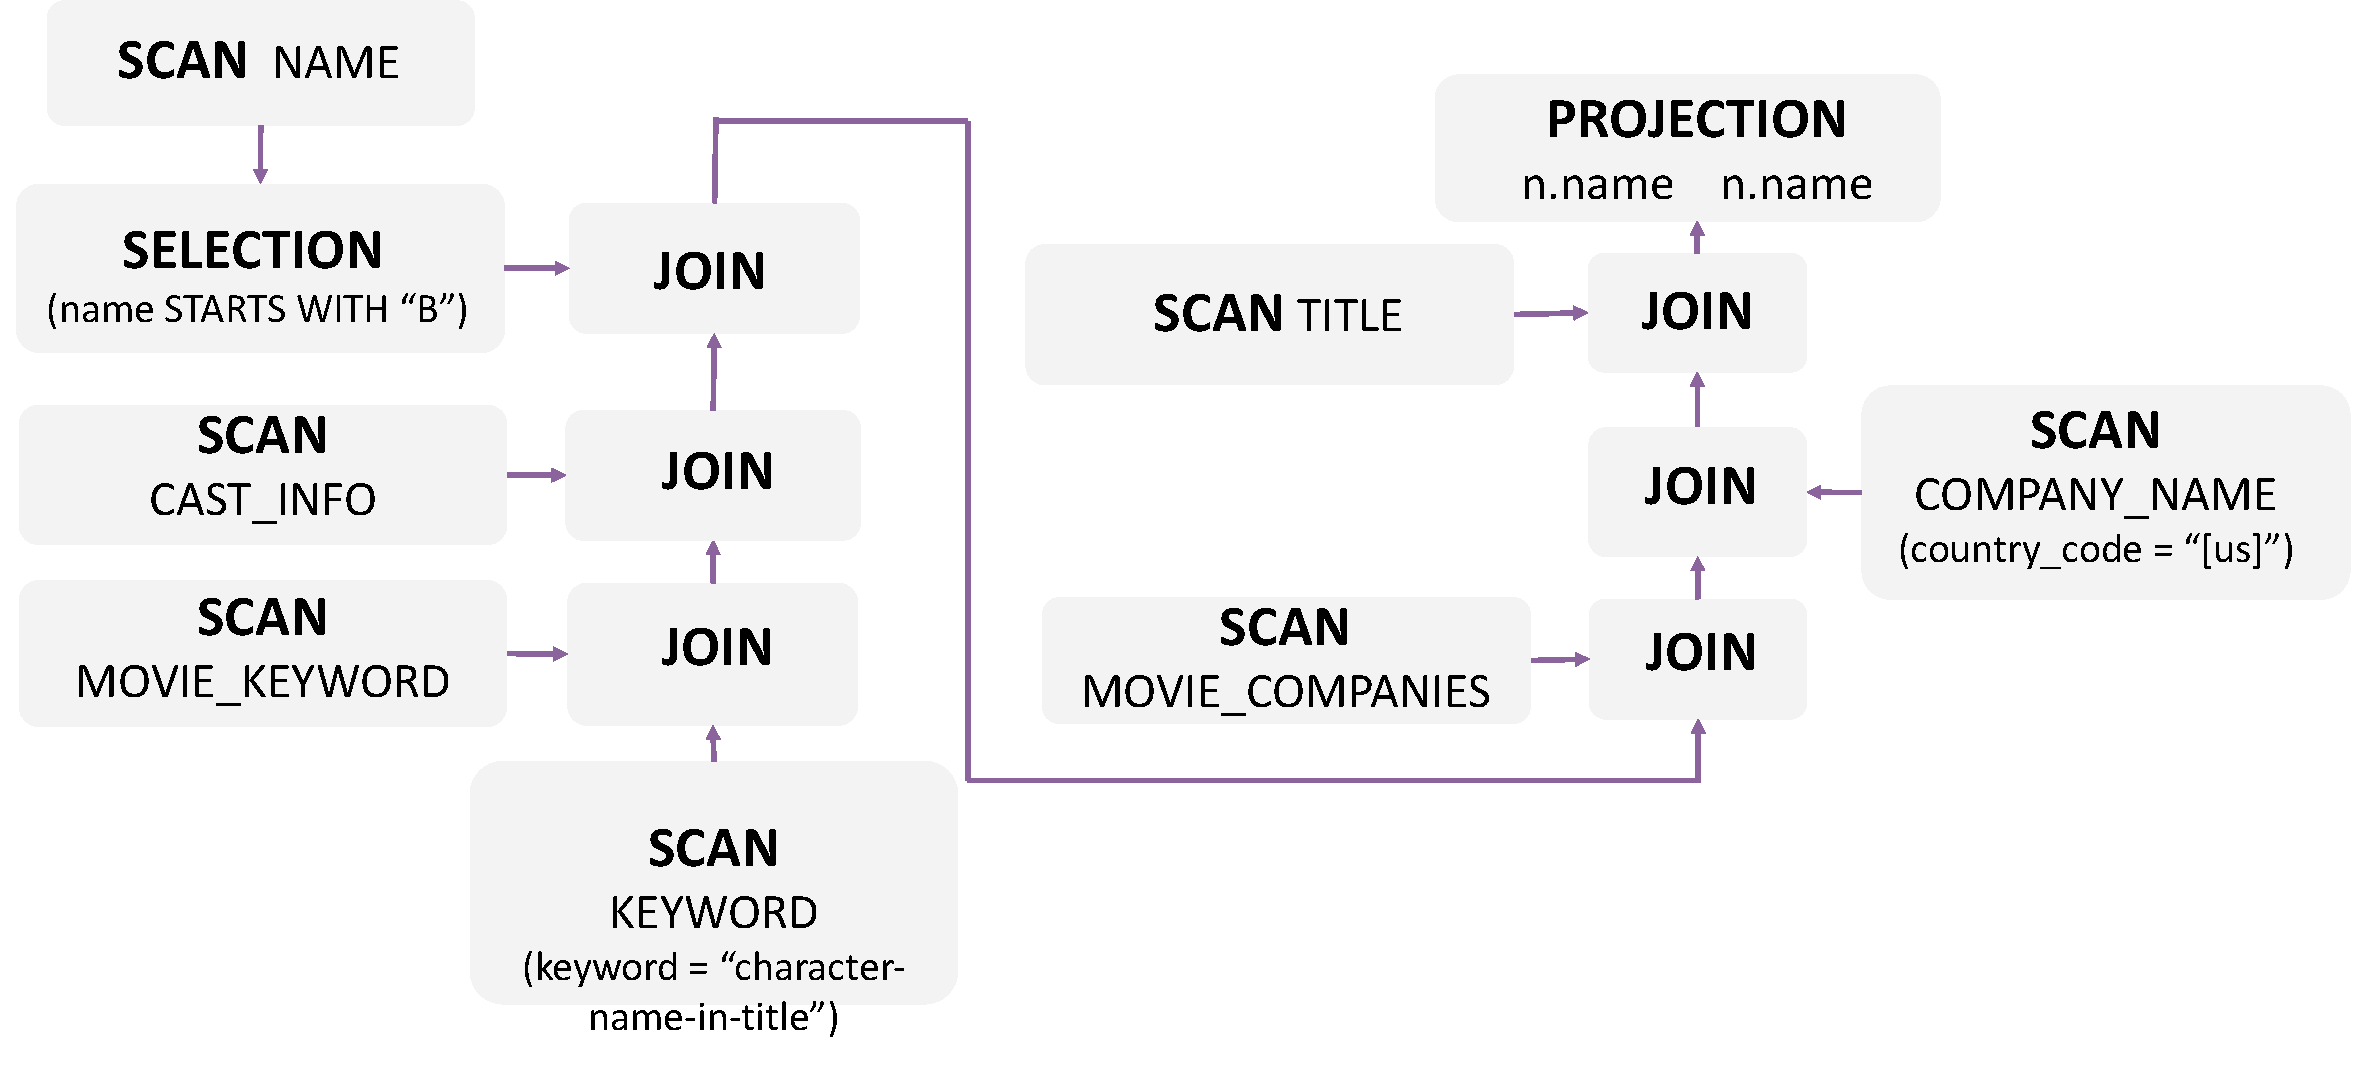
\includegraphics[width=\linewidth]{./figures/job17a-plan-umbra.pdf}
        \caption{Query Plan of Umbra}
        \label{fig:job17a-plan-umbra}
    \end{subfigure}
    \caption{Query plans of JOB[17] generated by \name, GrainDB, and Umbra.}
    \label{fig:job17a-query-plans}
\end{figure*}


\subsection{Case Study}
\revise{To further illustrate why the plans generated by \name are better than those generated by the baseline optimizers, we conduct a case study using the JOB[17] query as an example.
The query is shown in \reffig{job17-query}.
Specifically, the query plans optimized by \name, GrainDB, and Umbra for this query are shown in \reffig{job17a-query-plans}}.


The \revise{plan of \name starts from $\relation{\text{keyword}}$.
According to the plan, the results of scanning $\relation{\text{keyword}}$ expand to $\relation{\text{title}}$, $\relation{\text{company\_name}}$, and $\relation{\text{\name}}$ in sequence.
Please note that when $\mathcal{P}_{\name}$ expands from $\relation{\text{keyword}}$ to $\relation{\text{title}}$, an \expandedge~ operator followed by \getvertex~ operator is generated.
Then, \joinfuserule~ is applied to merge these two operators into an \expand~ operator. 
The \expand~ operator is implemented as a predefined join utilized in GrainDB that efficiently retrieve the neighboring vertices based on the VE-index}.

However, \revise{because GrainDB and Umbra apply relational optimizers, it is not necessary for them to join vertex relations and edge relations alternately. Consequently, they may miss opportunities to achieve better execution plans using the \joinfuserule, and cannot merge join operators such as $\relation{\text{keyword}} \bowtie \relation{\text{movie\_keyword}}$ and $\relation{\text{movie\_keyword}} \bowtie \relation{\text{title}}$}.

Moreover, \revise{the advantage of \name over baseline optimizers also stems from its support for the \expandintersect~ operation. For instance, given the IC[7] query, the execution plan generated by \name includes an EI-Join. This provides a significant advantage over the plans optimized by other optimizers}.
%\enlargethispage{1em}

\section{Related Work}
\label{sec:related-work}
%\textit{GetVertex}, \textit{GetEdge}, and \textit{GetNeighbor} are commonly used in graph queries.
%Specifically, \textit{GetVertex} is used to get the adjacent vertices of an edge, \textit{GetEdge} returns the edges from or to a given vertex, and \textit{GetNeigbor} gets the neighbors of a given vertex.
%Based on SQL/PGQ, in relational database, these operators can be implemented by joining tables representing vertices and edges.
%Then, it is crucial to support efficient join order optimization in the converged graph relational optimizer.

%In this section, we survey the query optimization techniques for relational databases and graph databases, respectively.
%Moreover, the mapping between relational data model and property graph
%Moreover, some relational databases (e.g., Oracle) allow users to create graph indices on relational tables.
%Then, researchers study to improve the performances of query execution with such graph indices.
%Therefore, this kind of works are also included in this section.
%These two types of works are also included in this section.

\stitle{Query Optimization for Relational Databases.} 
%Join order optimization was a traditional and crucial topic for query optimization in relational databases. 
%The order in which joins were conducted could influence the execution time significantly and had attained substantial accomplishments. 
Various studies of query optimization for relational databases were proposed to find the optimal join order.
Ibaraki et al.\cite{IbarakiK84} proved the NP-complexity of the join order optimization problem and designed an efficient algorithm with a time complexity of $O(n^2logn)$ to optimize tree queries.
%Ibaraki et al.\cite{IbarakiK84} proposed that there were usually fewer than ten tables involved in a typical query, and dealt with joins using nested-loops join. Specifically, they proved the NP-complexity of the join order optimization problem and designed an efficient algorithm with a time complexity of $O(n^2logn)$ to optimize tree queries.
Then, Krishnamurthy et al.\cite{optimize-nested-vldb-1986} optimized the algorithm and proposed an algorithm with a time complexity of $O(N^2)$ by reusing the computation results.
%Besides, the authors emphasized that since finding the optimal join order was a complex problem, it was more important to avoid the worst plan.
Moreover, Haffner et al.\cite{Haffnerjoinorder} converted the problem of join order optimization to that of finding the shortest path on directed graphs and solved the problem with the A* algorithm. 
%In detail, four heuristics were designed to estimate the remaining cost. 
%Furthermore, 
Kossmann et al.\cite{data-dependency-join} summarized the methods to optimize queries with data dependencies, such as uniqueness constraints, foreign key constraints, and inclusion dependencies.
\revise{Recently, researchers have attempted to incorporate worst-case optimal joins into generated plans to better handle queries containing cycles and reduce the size of intermediate results\cite{Aberger2016Sigmod,free-join}.
CLFTJ \cite{Kalinsky2017EDBT} introduces caching into trie join to reuse previously computed results.
Umbra \cite{umbra2020vldb} proposes a new hash trie data structure and further reduces the cost of set intersection}.
% Free Join \cite{free-join} unifies worst-case optimal joins and binary joins, achieving better performance than either of them alone}.
All these techniques can be orthogonally adopted in \name's relational optimization.

%Several studies have focused on improving cardinality estimation for cost computation, enabling cost-based optimizers to search for execution plans with potentially lower costs. A common approach is to estimate cardinality through sampling \cite{index-based-join-sampling,ripple-join,wanderjoin,index-based-join-sampling}. For instance, Li et al.\cite{wanderjoin} present an unbiased estimator based on random walks to estimate cardinalities. Leis et al.\cite{index-based-join-sampling} propose a computationally inexpensive method called index-based join sampling to improve accuracy. Other studies estimate cardinalities using histograms \cite{histogram,postgres-row-estimation}. These methods divide the values of a table column into several buckets to build a histogram and assume that the values are uniformly distributed within each bucket. The cardinality is then estimated by summing the number of values in the relevant buckets. Additionally, learning-based methods have been explored for cardinality estimation \cite{learning-based-estimation-1,learning-based-estimation-2,learning-based-estimation-3,learning-based-estimation-4}.


\comment{
Some researchers \cite{selinger,postgres-row-estimation} estimate the number of cardinalities by computing the selectivity of $A \bowtie_{A.col_1 = B.col_2} B$ as
\begin{equation*}
    \frac{1}{max(DV(A.col_1), DV(B.col_2))},
\end{equation*}
where $DV(A.col_1)$ is the number of distinct values of $A.col_1$ in table $A$.
}


\stitle{Query Optimization for Graph Databases.} Graph pattern matching, a fundamental problem in graph query processing, has been extensively studied~\cite{angles2017foundations}. In sequential settings, Ullmann's backtracking algorithm~\cite{ullmann1976algorithm} has been optimized using various techniques, such as tree indexing~\cite{shang2008quicksi}, symmetry breaking~\cite{han13turbo}, and compression~\cite{bi2016efficient}. 
%However, due to the challenges in parallelizing backtracking algorithms, 
Join-based algorithms have been developed for distributed environments. These algorithms use cost estimation to optimize join order, with binary-join algorithms\cite{lai2015scalable, lai2019distributed} estimating costs using random graph models and worst-case-optimal join algorithms~\cite{ammar2018distributed} ensuring a worst-case upper bound on the cost. Hybrid approaches\cite{mhedhbi2019optimizing, huge} adaptively select between binary and worst-case optimal joins based on the lower cost. 
\revise{Kùzu \cite{jin2023cidr} estimates the cost with the number of factorized tuples due to its factorized query processor}.
Recent studies have focused on improving cost estimation in graph pattern matching, including decomposing graphs into star-shaped subgraphs~\cite{cset} and comparing different cardinality estimation methods~\cite{gcare}. Some optimizers, like GLogS~\cite{GLogS}, search for the optimal plan by representing edges as binary joins or vertex-expansion subtasks. %and computing the plan bottom-up to obtain a worst-case optimal plan.
We follow the join-based methods such as~\cite{huge,GLogS} due to their compatibility with the relational context for which \name~ is designed. %However, to ensure seamless integration with the relational environment, we need to make adaptations to these methods accordingly.


\stitle{Bridging Relational and Graph Models.} There is a growing interest in studying the interaction between relational and graph models.
DuckPGQ~\cite{DuckPGQ,DuckPGQ-VLDB} has demonstrated support for SQL/PGQ within the DuckDB~\cite{duckdb}, utilizing the straightforward, graph-agnostic approach to transform and process pattern matching.
\revise{Since DuckPGQ converts SQL/PGQ queries into standard SQL query plans, it loses the opportunity to optimize the query from a graph query perspective}.
Index-based methods, such as GQ-Fast \cite{gqfast} and GRainDB \cite{graindb}, work towards construct graph-like index on relational databases to improve the performance of join execution. \name leveraged GRainDB's indexing technique for implementing physical graph operations. In contrast, methods like GRFusion \cite{GRFusion} and Gart~\cite{gart} work towards materializing graph from the relational tables,
so that graph queries can be executed directly on the materialized graph. Such methods incur additional storage costs and potential inconsistencies between relational and graph data.
%We prefer index-based techniques over materialization techniques due to their ability to work seamlessly with relational databases. % GRFusion builds an in-memory graph view based on relational tables and supports queries on both tables and graph views. This allows some relational joins to be replaced with graph traversals, enabling the application of graph-level optimizations. Similarly, in the work of Gart, the authors develop ETL tools to convert and import relational data into a graph store, upon which any graph processing system can be plugged in for efficient graph analysis. We prefer index-based techniques over materialization techniques due to their ability to work directly with relational databases, avoid additional storage costs, and ensure consistency between relational and graph data, making them more suitable for the relational context in which \name operates.



%In terms of translation-based methods, Apache/Age \cite{apache-age} is a typical work.
%Apache/Age is an extension of PostgreSQL, and it provides the ability to handle hybrid queries including openCypher and SQL.
%In detail, after a graph is created, a namespace with the same name as the graph is created.
%The vertices and edges in the graph are stored in corresponding tables in the namespace.
%When a query with both openCypher and SQL statements is performed, Apache/Age transforms the openCypher statements and converts the operators to those in PostgreSQL (e.g., MATCH PATH $\rightarrow$ join), and then the query is solved by PostgreSQL.
%It seems that Apache/Age is more like a syntactic sugar, and the advantanges of graphs and graph optimizers are not utilized.

%In terms of index-based methods, these methods build graph indices on relational databases, and attempt to accelerate queries with the indices.



\section{Conclusions}
\label{sec:conclusions}

\bibliographystyle{ACM-Reference-Format}
\bibliography{sample}

\end{document}
\endinput
